\documentclass[11pt]{article}
\usepackage[a4paper,margin=2.6cm,headheight=14pt]{geometry}
\usepackage[T1]{fontenc}
\usepackage{mathpazo}
\usepackage{microtype}
\usepackage{amsmath,amssymb,amsthm,bm,mathtools}
\usepackage{graphicx,booktabs,tabularx,multirow,array,longtable}
\usepackage{xcolor}
\usepackage[font=small,labelfont=bf]{caption}
\usepackage{subcaption}
\usepackage{enumitem}
\usepackage{fancyhdr}
\usepackage{tikz}
\usetikzlibrary{arrows.meta,positioning,calc,decorations.pathreplacing,shapes.geometric,fit,backgrounds,patterns}
\usepackage[ruled,vlined,linesnumbered]{algorithm2e}
\usepackage{tcolorbox}
\tcbuselibrary{skins,breakable}
\definecolor{headblue}{HTML}{1F5F8B}
\definecolor{boxgray}{HTML}{F4F6F8}
\definecolor{accred}{HTML}{B03A2E}
\definecolor{accgreen}{HTML}{2E7D32}
\definecolor{accorange}{HTML}{D68910}
\usepackage[colorlinks=true,linkcolor=headblue,citecolor=headblue,urlcolor=headblue]{hyperref}
\usepackage{titlesec}
\titleformat{\section}{\normalfont\Large\bfseries}{\thesection.}{0.6em}{}
\titleformat{\subsection}{\normalfont\large\bfseries}{\thesubsection}{0.6em}{}
\titleformat{\subsubsection}{\normalfont\normalsize\bfseries}{\thesubsubsection}{0.6em}{}
\pagestyle{fancy}
\fancyhf{}
\fancyhead[L]{\small\color{gray}Residual Monte Carlo with a Random-Ray Field in OpenMC}
\fancyfoot[C]{\thepage}
\renewcommand{\headrulewidth}{0pt}
\setlength{\parskip}{0.45em}
\setlength{\parindent}{0pt}
\setlist{itemsep=0.15em,topsep=0.3em}

% Notation
\newcommand{\vr}{\mathbf r}
\newcommand{\vO}{\boldsymbol\Omega}
\newcommand{\E}{\mathbb E}
\newcommand{\Var}{\operatorname{Var}}
\newcommand{\dd}{\,\mathrm d}
\newcommand{\Qmg}{Q^{\mathrm{MG}}}
\newcommand{\G}{\mathcal G}
\newcommand{\K}{\mathcal K}
\newcommand{\B}{\mathcal B}
\newcommand{\Wabs}{W_{\mathrm{abs}}}
\newcommand{\code}[1]{\texttt{\small #1}}
\newtheorem{proposition}{Proposition}
\newtheorem{lemma}{Lemma}
\theoremstyle{definition}
\newtheorem{definition}{Definition}
\newtcolorbox{keybox}[1][]{enhanced,breakable,colback=boxgray,colframe=headblue!60,boxrule=0.5pt,arc=1pt,left=6pt,right=6pt,top=4pt,bottom=4pt,fonttitle=\bfseries\small,title={#1}}
\newtcolorbox{intuition}{enhanced,breakable,colback=white,colframe=accorange!70,boxrule=0.5pt,arc=1pt,left=6pt,right=6pt,top=4pt,bottom=4pt,fonttitle=\bfseries\small,title={Intuition}}
\tikzset{
  box/.style={draw=headblue,fill=boxgray,rounded corners=2pt,align=center,font=\small,inner sep=4pt},
  arr/.style={-{Stealth[length=2.2mm]},thick,color=headblue},
  note/.style={font=\footnotesize,align=center,text=black!75},
}

\begin{document}
\thispagestyle{empty}
{\Large\bfseries Residual Monte Carlo with a Random-Ray Field in OpenMC:\\[2pt]
Method, Nuclear Data, Implementation, and First Measurements\par}
\vspace{0.6em}
{\itshape How a multigroup random-ray solution is corrected to continuous-energy accuracy by
signed Monte Carlo particles; why each estimator is unbiased; what controls its variance and
cost; how the nuclear data enter; and how the pieces sit inside OpenMC\par}
\vspace{0.6em}
14 November 2026\par
\vspace{1em}
\tableofcontents
\clearpage

\section*{Summary}
\addcontentsline{toc}{section}{Summary}

\paragraph{The method.} Residual Monte Carlo (RMC) solves the continuous-energy (CE) transport
eigenvalue problem in two layers:
\begin{itemize}
\item a multigroup (MG) random-ray solution, the \emph{field}, which gets most of the answer cheaply;
\item a signed Monte Carlo correction, which supplies what the field cannot represent.
\end{itemize}
The correction is driven by the field's \emph{residual}: the difference between the CE production of
the field's flux and the MG emission density the field assumed. Particles are sampled from that
residual and transported with OpenMC's own physics. Because the residual has both signs, so do the
particles. The correction's variance is meant to scale with the residual, not with the solution;
Part~\ref{part:method} shows why each estimator is unbiased and what sets its variance.

\paragraph{What has been built.} Inside OpenMC (C++ with a C API, driven from Python), the
implementation has the following components:
\begin{itemize}
\item the frozen field and its backward-characteristic reconstruction;
\item the residual estimators, by the density route and the density-free sampler route;
\item forward flights through OpenMC's collision physics;
\item the emission-source iteration;
\item three sign-cancellation methods: binned netting, destination pooling and a regional point
  kernel;
\item correction tallies.
\end{itemize}
Each piece is checked against stock OpenMC in isolation; see Appendix~\ref{app:gates} for the gates.

\paragraph{What was measured.} The first end-to-end run is on a graphite pincell against OpenMC's CE
eigenvalue calculation (Sections~\ref{sec:res:stage8} and~\ref{sec:res:followup}).
\begin{itemize}
\item \textbf{Stability.} The method is stable only with binned netting. Without it the bank's
  absolute weight grows geometrically and the run fails within 30 generations.
\item \textbf{Shape.} The fission-rate shape is unbiased with the CE correction tally.
\item \textbf{Eigenvalue bias.} Nine independent replicas give $+1050\pm360$~pcm at $N=2000$ residual
  samples per tag, and $N=16000$ gives $+600\pm280$~pcm. Neither a pure $1/N$ normalization bias nor
  netting's within-group smearing in the resonance range explains it alone.
\item \textbf{Figure of merit.} Relative to OpenMC it is $0.0018$ for $k$ ($0.0033$ at $N=16000$)
  and about $0.001$ for the fission shape. After the engineering of Part~\ref{part:impl} the
  projection is about $0.01$.
\item \textbf{Where the noise comes from.} The residual estimator dominates the noise. The
  scattering residual injects about 7 units of absolute weight per unit of fission production every
  generation. Part of that is an amplitude term that following amplitudes ($b=a$) remove; the rest is
  the high term's integration noise.
\item \textbf{History-based flights.} Making generations fission-to-fission is stable only with
  $b=a$ and about 30 times more residual samples per generation, and its figure of merit is 9 times
  lower. Measured in neutron lifetimes, the collision iteration's correlation is already short.
\end{itemize}

\paragraph{Verdict.} Optimization alone will not make the method competitive. Neither the iteration's
structure nor its normalization changes that. Feasibility depends on making each residual sample
about two orders of magnitude quieter per unit cost, for example with stratified incident directions
and a CE/MG control on shared incident energies. The bias must also be settled.
\clearpage

\part{The method}\label{part:method}

\section{Purpose and how to read this document}

This document describes, from the transport equation upward, a hybrid method that computes
continuous-energy (CE) eigenvalue solutions by \emph{correcting} a cheap multigroup (MG) random-ray
solution with Monte Carlo. It has four parts.

\begin{enumerate}
\item \textbf{The method} (this part): the mathematics and the intuition of every stage, the
  estimators grouped into classes, why each is unbiased, and what sets its variance and cost.
\item \textbf{Results}: every test that has been run, with its setup, what it shows, and the first
  end-to-end measurement against a CE Monte Carlo reference, including a figure of merit and its
  projection after optimization.
\item \textbf{Nuclear data}: the reactions, how they are represented and stored, how they shape
  real spectra, how OpenMC samples each one, and how each one constrains this method.
\item \textbf{Implementation}: the structure of the code inside OpenMC, its data containers and
  algorithms, and the performance consequences of each design choice.
\end{enumerate}

Mathematics comes first in each section, then pseudocode, then the implementation. Boxes labelled
\emph{Intuition} give the physical picture; boxes with a title state results that later sections
rely on. The notation is collected in Appendix~\ref{app:notation}. The code lives on the
\code{rmc} branch of an OpenMC fork, in \code{include/openmc/rmc}, \code{src/rmc},
\code{openmc/lib/rmc.py} and \code{examples/rmc}; the version-controlled methods chapter is
\code{docs/source/methods/rmc.rst} and the development log \code{docs/source/devguide/rmc.rst}.

\section{Transport background and notation}\label{sec:background}

\subsection{The phase space and the flux}

A neutron is described by its position $\vr$, its kinetic energy $E$ and its direction of flight
$\vO$ (a unit vector). The \textbf{angular flux} $\psi(\vr,E,\vO)$ is the neutron density times
speed, per unit volume, energy and solid angle; the \textbf{scalar flux} is
$\phi(\vr,E)=\int_{4\pi}\psi\dd\Omega$. A reaction rate density is a cross section times the flux:
$\Sigma_x(\vr,E)\,\phi(\vr,E)$ reactions per unit volume, time and energy. The macroscopic cross
section $\Sigma_x=\sum_i N_i\sigma_{x,i}$ sums the microscopic cross sections $\sigma_{x,i}$ of the
nuclides $i$ in the material, weighted by their atom densities $N_i$.

\subsection{The emission density}

The quantity at the centre of this method is not the flux but the \textbf{emission density}
$Q(\vr,E,\vO)$: the rate at which neutrons \emph{leave} collisions (or are born) at a point of phase
space. It has two parts, which we keep separate and call \emph{tags}:
\begin{align}
Q_s(\vr,E,\vO) &= \int\!\!\int \Sigma_s(\vr; E'\to E, \vO'\to\vO)\,\psi(\vr,E',\vO')\dd E'\dd\Omega',
\label{eq:Qs}\\
Q_f(\vr,E,\vO) &= \frac{1}{4\pi}\,\frac{1}{k}\int \chi(\vr; E\mid E')\,\nu\Sigma_f(\vr,E')\,\phi(\vr,E')\dd E'.
\label{eq:Qf}
\end{align}
$\Sigma_s(E'\to E,\vO'\to\vO)$ is the double-differential \emph{production} kernel of every
non-fission reaction with outgoing neutrons (elastic scattering, inelastic scattering,
$(n,2n)$, \dots), including their multiplicities; $\chi(E\mid E')$ is the fission spectrum and
$\nu\Sigma_f$ the fission neutron production. Fission emission is isotropic. The factor $1/k$ is the
eigenvalue normalization: in the $k$-eigenvalue problem the number of fission neutrons is divided by
$k$ so that a steady state exists.

\subsection{Two operators: flight and collision}

Write the transport equation as
\begin{equation}
\vO\cdot\nabla\psi + \Sigma_t\psi = Q_s + Q_f .
\end{equation}
Given an emission density $Q$, the flux it produces before any further collision is obtained by
integrating along the characteristic (the straight line) ending at $(\vr,\vO)$:
\begin{equation}\label{eq:G}
\psi(\vr,E,\vO) = (\G Q)(\vr,E,\vO) = \int_0^\infty e^{-\tau(\vr,\vr-s\vO;E)}\;Q(\vr-s\vO,E,\vO)\dd s ,
\end{equation}
where $\tau$ is the optical depth along the path. $\G$ is the \textbf{flight} (or first-flight, or
streaming) operator. The \textbf{collision} operator $\mathcal P(k)$ turns a flux into the next emission
density through equations \eqref{eq:Qs}--\eqref{eq:Qf}. Their product
\begin{equation}
\B(k)=\mathcal P(k)\,\G
\end{equation}
maps one \emph{generation} of emission to the next: where neutrons leave collisions now, to where
they leave their next collision. The CE eigenvalue problem is the fixed point
\begin{equation}
Q=\B(k)\,Q, \qquad \text{with } \langle\nu\Sigma_f,\G Q\rangle\text{ fixed},
\end{equation}
and $k$ is the value for which it has a positive solution. Analog Monte Carlo is the stochastic
version of iterating $\B$: each history samples a flight and a collision, again and again.

\begin{intuition}
An emission density is a ``where neutrons start'' map. Applying $\G$ smears each start along its
direction of flight with exponential attenuation; applying $\mathcal P$ turns the resulting flux
into new starts by scattering (which mostly lowers the energy) and fission (which restarts
neutrons at MeV energies). One power of $\B$ is one link in every neutron's chain of collisions.
\end{intuition}

\subsection{Monte Carlo estimators, variance and figure of merit}

An \textbf{estimator} is a random variable whose expectation is the quantity sought; it is
\textbf{unbiased} if the equality is exact. If one sample has variance $V$ and costs $C$ seconds, the
average of $N$ samples has variance $V/N$ and costs $NC$, so reaching a root-mean-square error
$\varepsilon$ costs $VC/\varepsilon^2$. The \textbf{figure of merit} $\mathrm{FOM}=1/(\sigma^2T)$ is
the inverse of $VC$: halving the variance at equal time doubles it. Every comparison in this document
is ultimately a comparison of $VC$.

A set of weighted particles $\{(x_i,w_i)\}$ with $x_i=(\vr_i,E_i,\vO_i)$ \emph{represents} a
(signed) measure $\mu$ if $\E[\sum_iw_iv(x_i)]=\int v\dd\mu$ for every response $v$. A particle bank
is a random object whose average, tested against any response, is the source it stands for. Its
\textbf{absolute weight} $\Wabs=\sum_i|w_i|$ is what sets the noise of every tally made from it: a
bank of $+1$ and $-1$ particles with zero net weight still carries noise of size $\Wabs$.

\section{The idea: a deterministic field plus a Monte Carlo correction}\label{sec:idea}

\subsection{Splitting the emission density}

A multigroup random-ray solve gives, cheaply and with little noise, an emission density that is
\emph{almost} right. Call it the \textbf{field} $Q^F$. The CE truth differs from it by a small signed
correction:
\begin{equation}
Q = Q^F + \delta Q .
\end{equation}
The correction is carried by a bank of signed Monte Carlo particles. One generation updates both
parts:
\begin{equation}\label{eq:update}
Q_{n+1} = \B(k_n)\,Q_n = \underbrace{\B Q^F_n - F_{n+1}}_{\text{residual }\widehat R_n} + F_{n+1}
 + \underbrace{\B\,\delta Q_n}_{\text{flights}} .
\end{equation}
$F_{n+1}$ is the part of the new emission that is kept in the field (with a frozen shape, the same
MG emission times amplitudes); the rest goes to the bank. The bank's update has two pieces:
\begin{itemize}
\item the \textbf{residual} $\B Q^F - F$: the CE emission the field produces in one generation,
  minus what the field already says. If the field were the exact CE solution this would be zero;
  for a good MG field it is small and signed;
\item the \textbf{flights}: the existing correction particles carried one generation forward by
  analog CE transport.
\end{itemize}

\begin{figure}[t]\centering
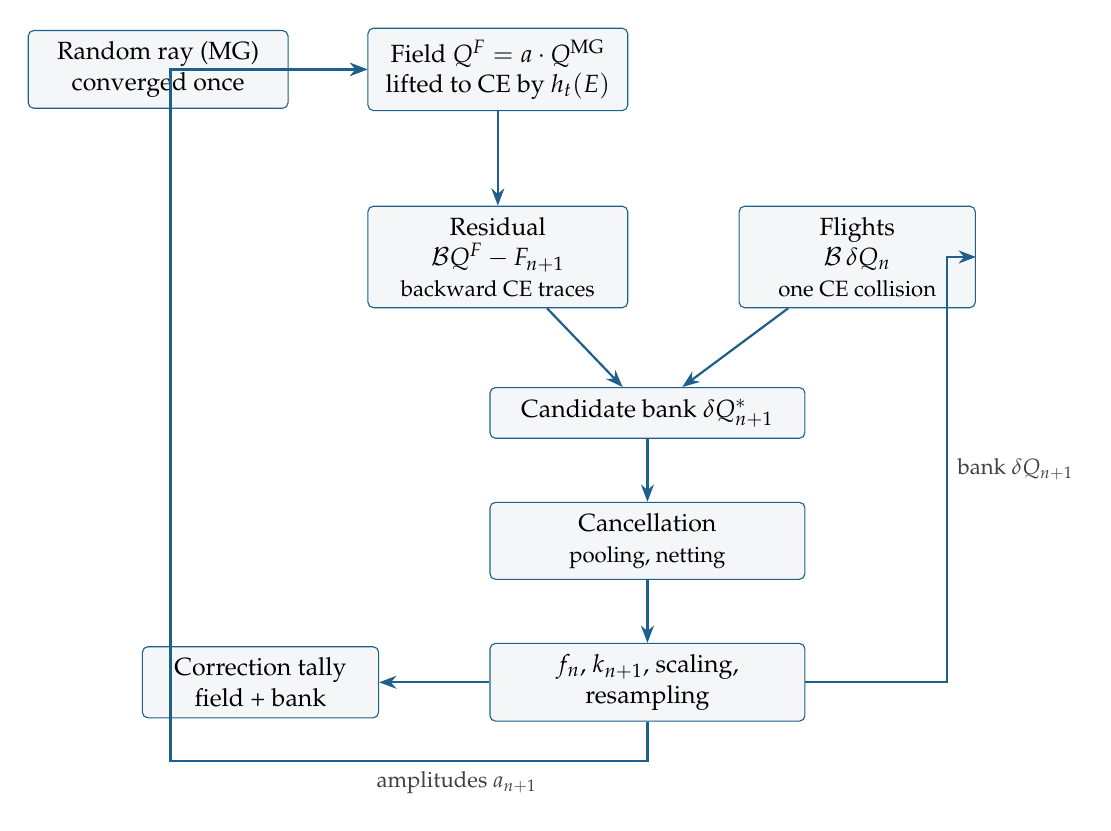
\begin{tikzpicture}[node distance=7mm and 10mm]
\node[box,minimum width=33mm] (rr) {Random ray (MG)\\ converged once};
\node[box,right=of rr,minimum width=33mm] (field) {Field $Q^F=a\cdot\Qmg$\\ lifted to CE by $h_t(E)$};
\node[box,below=12mm of field,minimum width=33mm] (res) {Residual\\ $\B Q^F - F_{n+1}$\\ \footnotesize backward CE traces};
\node[box,right=14mm of res,minimum width=30mm] (fl) {Flights\\ $\B\,\delta Q_n$\\ \footnotesize one CE collision};
\node[box,below=10mm of res,xshift=19mm,minimum width=40mm] (cand) {Candidate bank $\delta Q^\ast_{n+1}$};
\node[box,below=8mm of cand,minimum width=40mm] (canc) {Cancellation\\ \footnotesize pooling, netting};
\node[box,below=8mm of canc,minimum width=40mm] (norm) {$f_n$, $k_{n+1}$, scaling,\\ resampling};
\node[box,left=14mm of norm,minimum width=30mm] (tally) {Correction tally\\ field + bank};
\draw[arr] (rr)--(field);
\draw[arr] (field)--(res);
\draw[arr] (res)--(cand);
\draw[arr] (fl)--(cand);
\draw[arr] (cand)--(canc);
\draw[arr] (canc)--(norm);
\draw[arr] (norm.east) -- ++(18mm,0) |- node[note,pos=0.25,right]{bank $\delta Q_{n+1}$} (fl.east);
\draw[arr] (norm.west) -- (tally.east);
\draw[arr] (norm.south) -- ++(0,-5mm) -| node[note,pos=0.2,below]{amplitudes $a_{n+1}$} ([xshift=-25mm]field.west) -- (field.west);
\end{tikzpicture}
\caption{One generation of the method. The field is a multigroup solution lifted to continuous
energy; the bank of signed CE particles carries what the field misses. Everything is driven by two
CE kernels: backward traces (residual) and forward one-collision flights.}\label{fig:overview}
\end{figure}

Figure~\ref{fig:overview} shows the loop. Its correctness is a one-line argument:
\begin{keybox}[Why the iteration is right]
If the residual and the flights are unbiased estimates of $\B Q^F_n-F_{n+1}$ and $\B\,\delta Q_n$,
then $\E[F_{n+1}+\delta Q_{n+1}]=\B(k_n)(Q^F_n+\E\delta Q_n)$: in expectation the method applies
exactly one CE generation per step. Everything the field gets wrong (group structure, flat sources,
P$_0$ scattering, self-shielding) is corrected by the bank, at a cost set by how much the field gets
wrong.
\end{keybox}

\subsection{Why it might pay off}

Analog Monte Carlo spends its particles on the whole emission density. This method spends them on
the residual, whose size is the field's error. If the residual can be estimated with noise
proportional to its own size, and if the bank stays small, the Monte Carlo variance scales with the
field's error rather than with the solution, as in multilevel Monte Carlo. Two things stand in the way,
and much of this document is about them:
\begin{enumerate}
\item \textbf{The residual's estimator must have residual-scale noise.} The difference
  $\B Q^F-F$ is small, but each of its terms is production-scale. Unless the two terms are evaluated
  so that their noise cancels, the estimate is as noisy as the production itself
  (Section~\ref{sec:residual}).
\item \textbf{Signed weights must cancel.} Particles never interact, so a positive and a negative
  particle at the same place do not annihilate by themselves; without cancellation $\Wabs$ grows
  with each generation (Section~\ref{sec:cancellation}).
\end{enumerate}

\section{Random ray in one section}\label{sec:randomray}

The field comes from OpenMC's random-ray solver, a stochastic method of characteristics. It solves
the MG transport equation with a flat (constant) emission in each source region:
\begin{enumerate}
\item \textbf{Rays.} Each batch launches rays from uniform points in a box with isotropic directions.
  A ray first travels a \emph{dead} length without tallying, so that its angular flux forgets its
  arbitrary starting value, then an \emph{active} length.
\item \textbf{Attenuation.} Along a segment of length $\ell$ in region $R$, with the region's MG source
  $Q_{R,g}/4\pi$, the angular flux changes exactly as
  $\psi_{out}=\psi_{in}e^{-\Sigma_{t,g}\ell}+\frac{Q_{R,g}}{4\pi\Sigma_{t,g}}(1-e^{-\Sigma_{t,g}\ell})$,
  and the segment's contribution to the region's scalar flux is the average of $\psi$ over it, times
  $\ell$.
\item \textbf{Region flux.} Summing over segments and dividing by the total track length per unit
  volume gives $\bar\phi_{R,g}$; a power iteration updates $Q$ and $k$ from it.
\end{enumerate}
The method is \emph{biased} by the flat-source approximation and the multigroup cross sections, and
noisy because the rays are random; averaging many batches removes the noise but not the
discretization. That discretization error is exactly what the residual measures. In this method
random ray is used twice: once, to produce the field; and, optionally, every generation as a
\emph{sweep} whose segments serve as quadrature directions and whose region emission
$\hat Q$ is the MG update of the field (tandem estimators).

\begin{figure}[t]\centering
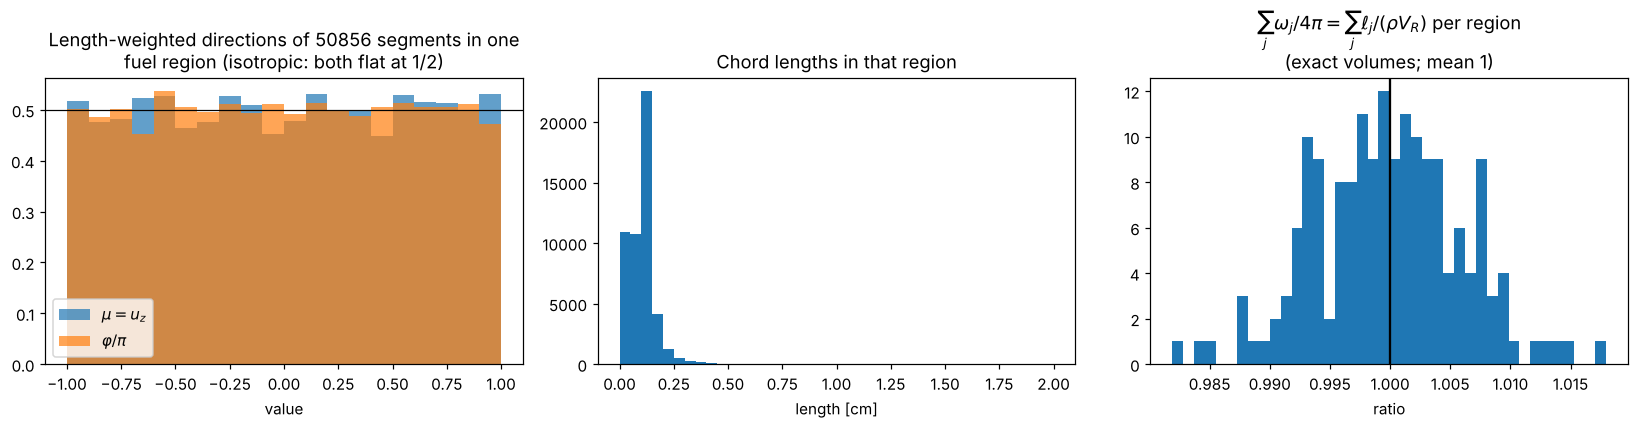
\includegraphics[width=0.8\textwidth]{figures/segments.png}
\caption{Segments of a random-ray sweep crossing one source region: each carries a direction, a chord
length and a chord-averaged MG angular flux; with weights $\omega_j=4\pi\ell_j/(\rho V_R)$ they form an
unbiased quadrature of the angular integral at points of the region.}\label{fig:segments}
\end{figure}

\section{The frozen field}\label{sec:field}

\subsection{From random ray to a continuous-energy emission density}

The random-ray solve (OpenMC's own solver) uses flat sources in \emph{source regions} $R$ (a cell, or
a cell cut by a mesh) and $G$ energy groups. It returns region-group scalar fluxes $\bar\phi_{R,g}$,
from which the MG emission densities per unit volume (integrated over angle and group) follow:
\begin{equation}
Q_{s,R,g}=d_R\sum_{g'}\nu\Sigma_{s,m}(g'\to g)\,\bar\phi_{R,g'},\qquad
Q_{f,R,g}=d_R\,\frac{\chi_{m,g}}{k^{\mathrm{MG}}}\sum_{g'}\nu\Sigma_{f,m,g'}\,\bar\phi_{R,g'},
\end{equation}
with $m$ the region's material and $d_R$ its density multiplier. A CE method needs an emission at
every energy, so each group is \textbf{lifted} by a within-group shape:
\begin{equation}\label{eq:field}
\Qmg_t(\vr,E,\vO)=\frac{1}{4\pi}\,Q_{t,R(\vr),g(E)}\,h_{t,m,g}(E),\qquad \int_g h_{t,m,g}\dd E=1 .
\end{equation}
The lifts $h_s,h_f$ (and a flux shape $h^\phi$ used only for proposals) are histograms on a fine
energy grid, tallied once from a short CE run of the same material. The field is a
\emph{definition}: any choice of lifts gives a valid field, and a better choice only makes the
residual smaller. The amplitudes $a=(a_s,a_f)$ scale the two tags: $Q^F=a_s\Qmg_s+a_f\Qmg_f$.

\begin{figure}[t]\centering
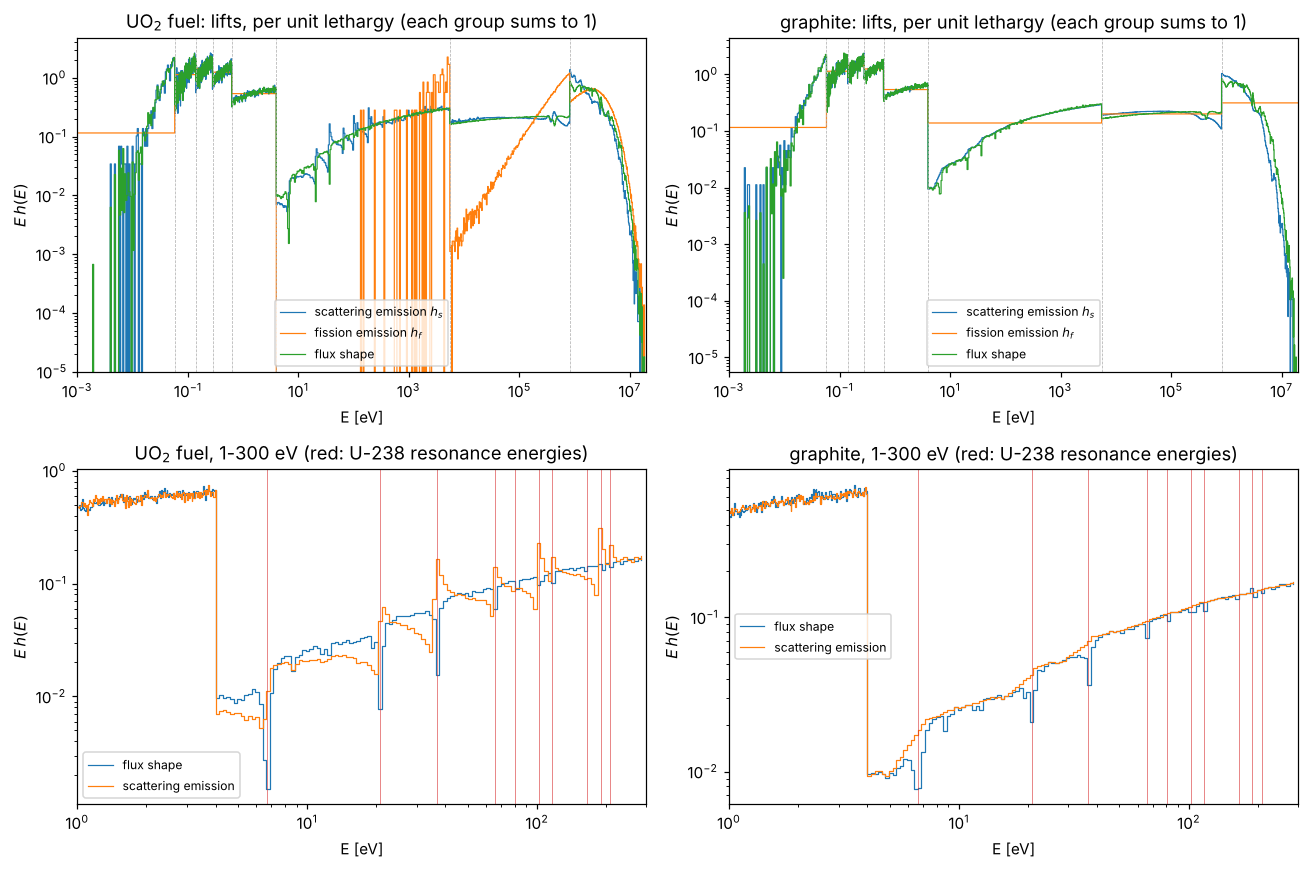
\includegraphics[width=0.92\textwidth]{figures/lifts.png}
\caption{Lifts of the graphite pincell: within-group shapes of the scattering emission, fission
emission and flux in the fuel and the graphite, on the fine grid (200 bins per group). The lifts carry
the resonance structure and the fission spectrum that eight groups cannot.}\label{fig:lifts}
\end{figure}

\subsection{Normalization and volumes}

The field is scaled to unit MG fission production, $\langle 1,\Qmg_f\rangle=\sum_RV_R\sum_gQ_{f,R,g}=
1/k^{\mathrm{MG}}$, so the iteration starts from $a_0=(1,1)$ and $k_0=k^{\mathrm{MG}}$. Region
volumes $V_R$ enter the normalization, the field's masses, the sweep weights and every exact integral
of the field. OpenMC's random ray can be given \emph{prescribed} volumes; with the exact volumes of the
source regions (each mesh voxel cut by the pin surface in closed form) the field and every reference
integral use the true geometry. With point-sampled volumes the small regions at the pin surface carry
a few per cent of error, which appears as apparent bias in any test that integrates the field exactly
(Section~\ref{sec:res:controlled}).

\section{The backward characteristic}\label{sec:backward}

\subsection{What is computed}

The residual needs the CE flux that the field produces at a chosen point, direction and energy:
equation~\eqref{eq:G} with $Q=Q^F$. Along the backward path $\vr(s)=\vr^\star-s\vO'$ (folded through
reflecting boundaries) the path crosses segments $k$ of length $\ell_k$, each in one region and one
material. With the field flat in a region and CE cross sections constant along a segment,
\begin{equation}\label{eq:psi}
\psi(\vr^\star,E',\vO')=\sum_k e^{-\tau_k(E')}\,q_k(E')\,
\frac{1-e^{-\Sigma_{t,k}(E')\ell_k}}{\Sigma_{t,k}(E')},\qquad q_k(E')=Q^F(R_k,E'),
\end{equation}
where $\tau_k$ is the optical depth from $\vr^\star$ to the near end of segment $k$. Two choices make
this cheap: the geometry is traced \emph{once} per direction and reused for every energy requested
on it, and the trace is extended lazily in chunks only while some energy is still alive.

\begin{figure}[t]\centering
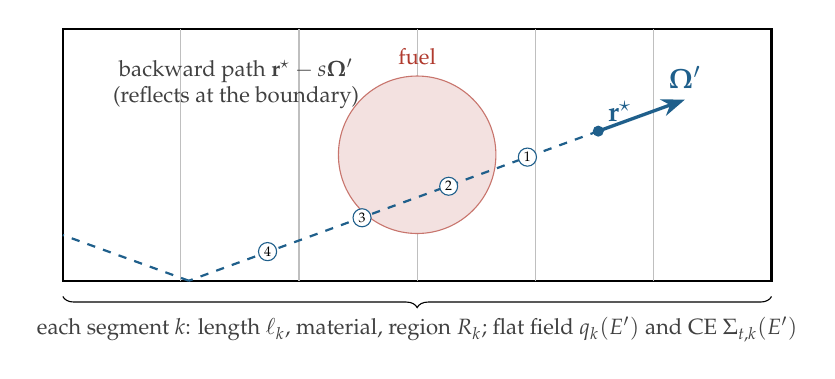
\begin{tikzpicture}[scale=1.0]
\draw[thick] (0,0) rectangle (9,3.2);
\foreach \x in {1.5,3,4.5,6,7.5} \draw[gray!50] (\x,0)--(\x,3.2);
\fill[accred!15] (4.5,1.6) circle (1.0);
\draw[accred!70] (4.5,1.6) circle (1.0);
\node[accred] at (4.5,2.85) {\footnotesize fuel};
\fill[headblue] (6.8,1.9) circle (2pt) node[above right] {$\vr^\star$};
\draw[-{Stealth},very thick,headblue] (6.8,1.9) -- (7.9,2.3) node[above] {$\vO'$};
\draw[thick,dashed,headblue] (6.8,1.9) -- (1.6,0.0);
\draw[thick,dashed,headblue] (1.6,0.0) -- (0,0.58);
\node[note] at (2.2,2.5) {backward path $\vr^\star-s\vO'$\\ (reflects at the boundary)};
\foreach \p/\l in {{(5.9,1.57)}/1,{(4.9,1.20)}/2,{(3.8,0.80)}/3,{(2.6,0.37)}/4} \node[circle,fill=white,draw=headblue,inner sep=0.8pt,font=\tiny] at \p {\l};
\draw[decorate,decoration={brace,amplitude=4pt,mirror}] (0,-0.2) -- (9,-0.2) node[midway,below=4pt,note] {each segment $k$: length $\ell_k$, material, region $R_k$; flat field $q_k(E')$ and CE $\Sigma_{t,k}(E')$};
\end{tikzpicture}
\caption{The backward characteristic from a destination $\vr^\star$ against the incident direction
$\vO'$: one geometric trace (here crossing a source-region mesh, the fuel pin and a reflecting face)
serves every incident energy requested on it.}\label{fig:backward}
\end{figure}

\subsection{Tails: why roulette is unbiased}

In a reflective problem the path never ends; it must be cut. Cutting at a fixed length biases the
estimate. \textbf{Roulette} does not: when the transmission $T=e^{-\tau}$ along the path falls below a
threshold $T_c$, the path continues with probability $T/T_c$ and with $T$ reset to $T_c$, or stops.
\begin{proposition}
For any $T_c>0$ the roulette estimate of \eqref{eq:psi} has the same expectation as the infinite sum.
\end{proposition}
\begin{proof}
Consider the contribution of the remaining path beyond the point where $T<T_c$ is first reached; it
is $T\cdot S$ with $S$ the (unattenuated-from-here) remainder. Roulette returns $T_c\,S'$ with
probability $T/T_c$ and $0$ otherwise, where $S'$ is the same construction applied recursively. By
induction $\E S'=S$, so the expectation is $(T/T_c)\,T_c\,S=T\,S$.
\end{proof}
The threshold therefore trades variance against cost and never moves the mean.
Figure~\ref{fig:backward_tails} compares the three tails implemented: vacuum (exact, only where paths
leave), roulette, and a fixed dead length (biased, no noise).

\begin{figure}[t]\centering
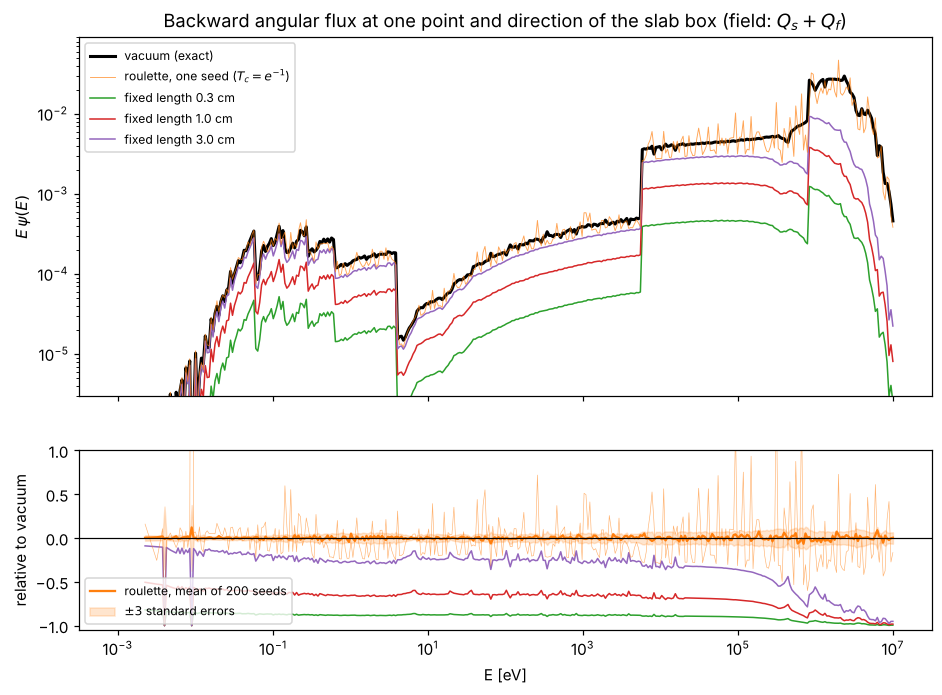
\includegraphics[width=0.85\textwidth]{figures/backward_tails.png}
\caption{Backward $\psi$ in the infinite medium with the three tails against the closed form
$q(E')/\Sigma_t(E')$. Roulette is unbiased at every threshold; its noise appears where the mean free
path is long compared with the geometry.}\label{fig:backward_tails}
\end{figure}

\section{Production at a common output}\label{sec:production}

\subsection{The problem}

The residual compares the CE emission produced by the field with the field itself \emph{at the same
outgoing state} $(\vr^\star,E,\vO)$. The CE emission there is the integral \eqref{eq:Qs}--\eqref{eq:Qf}
over incident energy and direction, with the backward $\psi$ as the incident flux. Over incident
directions we use a quadrature or random directions; over incident energy there are two very
different possibilities, which give the two \emph{routes} of every reaction.

\subsection{The evaluator route: densities}

If the production kernel has a known density in the outgoing variables, we can evaluate it at the
chosen output. For \textbf{fission}, emission is isotropic and the outgoing energy has density
$\chi(E\mid E')$; with one incident energy drawn from a proposal $g(E')$,
\begin{equation}\label{eq:fission_eval}
\int\!\!\int \frac{\chi(E\mid E')\nu\Sigma_f(E')}{4\pi k}\psi(E',\vO')\dd E'\dd\Omega'
\approx \sum_j\omega_j\,\frac{\nu\Sigma_f(E'_j)\,\chi(E\mid E'_j)\,\psi(\vr^\star,E'_j,\vO'_j)}{4\pi k\,g(E'_j)} .
\end{equation}
OpenMC can only sample $\chi$; the evaluator implements the density of exactly what OpenMC's sampler
does, including the interpolation between tabulated incident energies and the rescaling of outgoing
energies to interpolated endpoints (Section~\ref{sec:nd:openmc}).

For \textbf{elastic scattering off a stationary target} of mass ratio $A>1$, energy and angle are tied
by two-body kinematics: an incident neutron at $E'$ deflected by laboratory cosine
$\mu_0=\vO'\cdot\vO$ leaves with $E=E'\gamma_A(\mu_0)$, where
\begin{equation}
\gamma_A(\mu_0)=\left(\frac{\mu_0+\sqrt{A^2-1+\mu_0^2}}{A+1}\right)^2 .
\end{equation}
Given the output $(E,\vO)$ and an incident direction, there is exactly one incident energy that can
produce it, the \textbf{image} $E'=E/\gamma_A(\mu_0)$. The energy integral collapses onto it:
\begin{equation}\label{eq:elastic_image}
\int\K^{el}\psi\dd E'=\sum_iN_i\,\sigma_{el,i}(E'_i)\,
\frac{p_{lab,i}(\mu_0\mid E'_i)}{2\pi\,\gamma_{A_i}(\mu_0)}\,\psi(\vr^\star,E'_i,\vO'),
\qquad p_{lab}=p_{cm}(\mu_{cm}(\mu_0))\left|\frac{\dd\mu_{cm}}{\dd\mu_0}\right| .
\end{equation}
The Jacobian $1/\gamma$ converts the delta function in energy; $p_{lab}$ converts the tabulated
centre-of-mass angular distribution to the laboratory. No incident energy is sampled at all, so the
elastic evaluator has no energy-integration noise; its noise is in the incident direction.

\begin{figure}[t]\centering
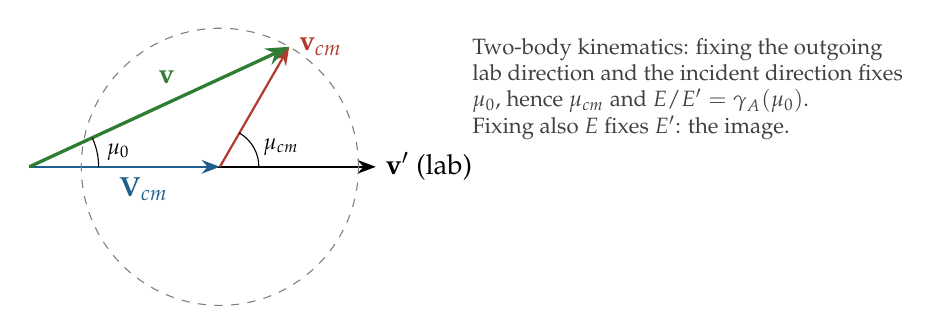
\begin{tikzpicture}[scale=1.1]
\draw[-{Stealth},thick] (0,0) -- (4,0) node[right] {$\mathbf v'$ (lab)};
\draw[-{Stealth},thick,headblue] (0,0) -- (2.2,0) node[below,pos=0.6] {$\mathbf V_{cm}$};
\draw[dashed,gray] (2.2,0) circle (1.6);
\draw[-{Stealth},thick,accred] (2.2,0) -- ({2.2+1.6*cos(60)},{1.6*sin(60)}) node[right] {$\mathbf v_{cm}$};
\draw[-{Stealth},very thick,accgreen] (0,0) -- ({2.2+1.6*cos(60)},{1.6*sin(60)}) node[above left,pos=0.6] {$\mathbf v$};
\draw (0.8,0) arc (0:{atan(1.6*sin(60)/(2.2+1.6*cos(60)))}:0.8) node[midway,right,font=\footnotesize] {$\mu_0$};
\draw ({2.2+0.45},0) arc (0:60:0.45) node[midway,right,font=\footnotesize] {$\mu_{cm}$};
\node[note,align=left] at (7.6,0.9) {Two-body kinematics: fixing the outgoing\\ lab direction and the incident
direction fixes\\ $\mu_0$, hence $\mu_{cm}$ and $E/E'=\gamma_A(\mu_0)$.\\ Fixing also $E$ fixes $E'$: the image.};
\end{tikzpicture}
\caption{Elastic scattering off a stationary target in velocity space. The centre-of-mass velocity
$\mathbf V_{cm}=\mathbf v'/(A+1)$; in the CM frame the neutron speed is unchanged and only its direction
is sampled. The lab outgoing velocity lies on the dashed circle.}\label{fig:kinematics}
\end{figure}

\subsection{The sampler route: OpenMC's own collision routines}

Every other channel (elastic scattering off a moving target, S($\alpha,\beta$), inelastic levels and
continuum, $(n,xn)$) is handled by OpenMC's own collision routine: draw $E'$ from $g$, choose a
sampler-route channel with probability proportional to its production
$\Sigma^{samp}_{\mathcal P}(E')$, call the routine on a scratch particle, and keep the outgoing state
as a new particle with weight
\begin{equation}\label{eq:sampler_weight}
c=\omega_j\,\frac{\Sigma^{samp}_{\mathcal P}(E')\,\psi(\vr^\star,E',\vO'_j)}{g(E')} .
\end{equation}
Its expectation is the sampler-route production at its own (random) outgoing state: correct by
construction for every law OpenMC supports. The price is that its state is \emph{not} the destination's
outgoing state, which matters for the residual (Section~\ref{sec:lowterm}).

\begin{keybox}[The channel registry]
Every reaction with outgoing neutrons is a \emph{channel} (nuclide, reaction, tag). At every incident
energy each channel is on exactly one route, so evaluator plus sampler production equals the tag's
total production and nothing is counted twice. Capture belongs to no channel but stays in $\Sigma_t$.
Stationary elastic and fission are on the evaluator route by default; with \code{all\_sampler} every
channel goes to the sampler route and the estimator needs no density at all.
\end{keybox}

\section{The residual estimator}\label{sec:residual}

\subsection{One residual sample}

The residual of tag $t$ is $R_t=\K_tQ^F-b_t\Qmg_t$ with $\K_t=\mathcal P_t\G$ the CE production of
tag $t$. One sample (Figure~\ref{fig:sample}):
\begin{enumerate}
\item \textbf{Destination.} $\vr^\star$ uniform in the field's box (or in regions weighted by volume
  or emission); locate its region $R$ and material $m$.
\item \textbf{Outgoing state.} $\vO$ isotropic, $E$ from a mixture of the region's emission spectrum
  and a log-uniform component (so that the support covers every $E$ where the residual can be
  nonzero). The sample's density is $\varrho=\pi(\vr^\star)\,p(E)/4\pi$.
\item \textbf{Directions.} $J$ incident directions $\vO'_j$ with weights $\omega_j$: a spherical
  Fibonacci set under a uniformly random rotation ($\omega_j=4\pi/J$), or the segments of a random-ray
  sweep crossing $R$.
\item \textbf{Traces.} One backward trace per direction; on it the incident energies of every
  evaluator (images for elastic, a drawn $E'$ for fission) and the sampler route's $K$ energies.
\item \textbf{Record.} The density-branch record stores the CE production at $(E,\vO)$ per source
  tag, $C_y$, the MG control $M_y$ and its restored mean $R_y$ (below), and the field value
  $U=\Qmg_t(\vr^\star,E)$. Sampler particles are separate records with their own state.
\end{enumerate}
The weight of a density record, for amplitudes $a,b$, eigenvalue $k$, control coefficient $c$ and
mixing $\lambda$, is
\begin{equation}\label{eq:weight}
w=\frac{1}{N\varrho}\Big\{\frac{\sum_ya_y\,(C_y-cM_y+cR_y)}{k^{[t=f]}}-b_t\big[(1-\lambda)U+
\lambda\,\tfrac{\sum_ya_yR_y}{k^{[t=f]}}\big]\Big\},
\end{equation}
and a sampler particle has $w=(\sum_ya_yC_y+Z)/(k^{[t=f]}N\varrho)$. The records do not depend on
$(a,b,k,c,\lambda)$: one set of samples serves every value, so variants can be compared on identical
random numbers and residuals can be generated ahead of the generation that uses them.

\begin{figure}[t]\centering
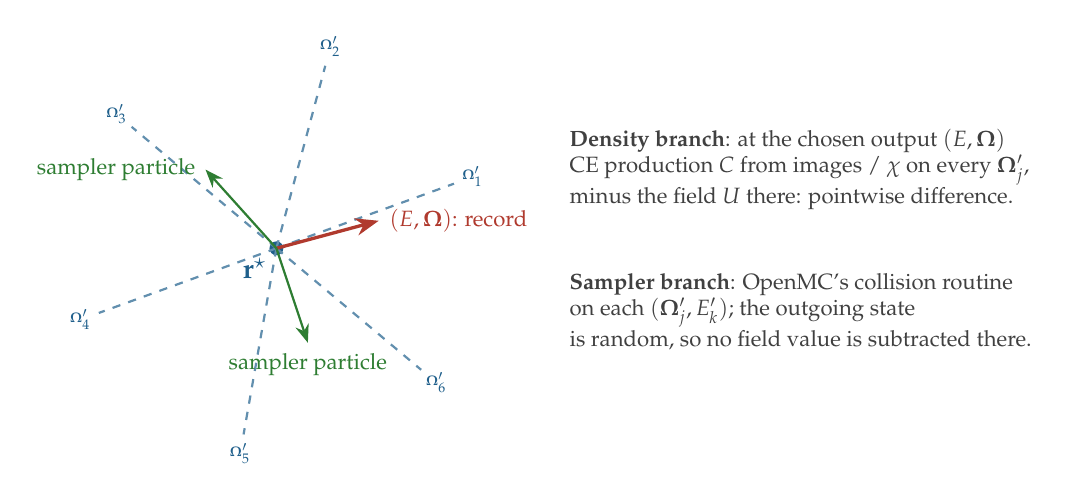
\begin{tikzpicture}[scale=1]
\fill[headblue] (0,0) circle (2.5pt) node[below left] {$\vr^\star$};
\foreach \a/\l in {20/1,75/2,140/3,200/4,260/5,320/6} {
  \draw[thick,headblue!70,dashed] (0,0) -- ({2.4*cos(\a)},{2.4*sin(\a)});
  \node[font=\tiny,headblue] at ({2.65*cos(\a)},{2.65*sin(\a)}) {$\vO'_{\l}$};
}
\draw[-{Stealth},very thick,accred] (0,0) -- (1.3,0.35) node[right,font=\footnotesize] {$(E,\vO)$: record};
\draw[-{Stealth},thick,accgreen] (0,0) -- (-0.9,1.0) node[left,font=\footnotesize] {sampler particle};
\draw[-{Stealth},thick,accgreen] (0,0) -- (0.4,-1.2) node[below,font=\footnotesize] {sampler particle};
\node[note,align=left,anchor=west] at (3.6,1.0) {\textbf{Density branch}: at the chosen output $(E,\vO)$\\
CE production $C$ from images / $\chi$ on every $\vO'_j$,\\ minus the field $U$ there: pointwise difference.};
\node[note,align=left,anchor=west] at (3.6,-0.8) {\textbf{Sampler branch}: OpenMC's collision routine\\ on each $(\vO'_j,E'_k)$; the outgoing state\\ is random, so no field value is subtracted there.};
\end{tikzpicture}
\caption{Anatomy of one residual sample: a destination, $J$ backward directions, one chosen output
state for the density branch, and sampler particles at their own states.}\label{fig:sample}
\end{figure}

\subsection{Proposals and their densities}

Every random choice in a sample returns its value and the density it was drawn from, and the weight
is formed only from that density. The choices and their densities:
\begin{itemize}
\item \textbf{Destination.} Uniform in the field's box ($\pi(\vr)=1/V_{box}$), or a region chosen with
  probability $\pi_R\propto V_R$ (or $V_R$ times a tabulated weight, or restricted to fissionable
  regions for tag $f$) and a uniform point in it ($\pi(\vr)=\pi_R/V_R$).
\item \textbf{Outgoing energy.} $p(E)=(1-\beta)\,p_{em}(E\mid R)+\beta\,p_{log}(E)$, with $p_{em}$ the
  region's lifted emission spectrum of the tag and $p_{log}$ log-uniform over the data range. The
  log-uniform part guarantees that $p>0$ wherever the residual can be nonzero (the CE emission can
  occupy energies where the field has none).
\item \textbf{Outgoing direction.} Isotropic, $1/4\pi$.
\item \textbf{Incident energy} on the sampler route and for fission: log-uniform, or led by the
  direction's own MG flux (a mixture of its group shape and log-uniform), or from the region's lifted
  flux.
\end{itemize}
A proposal affects only the variance, provided it covers the support of the integrand; that condition
is checked by the infinite-medium gates, which compare the means with closed forms including windows
where the integrand is concentrated (thermal fission, the U-238 resolved resonances).

\subsection{The sweep quadrature and the track-length identity}

With sweep directions the quadrature weights are $\omega_j=4\pi\ell_j/(\rho V_R)$, where $\ell_j$ is the
chord length of segment $j$ in region $R$ and $\rho$ the total track length per unit volume of the sweep.
For rays with uniform starting points and isotropic directions, the expected track length of rays in
direction $\dd\Omega$ through region $R$ is $\rho V_R\dd\Omega/4\pi$, so
$\E[\sum_{j\in R}\omega_jf(\vO'_j)]=\int f\dd\Omega'$ for any $f$: the segments are an unbiased
quadrature of the angular integral, exactly when $V_R$ is the true volume. The CE trace then follows a
new characteristic from the destination parallel to segment $j$; what is shared with the sweep is the
direction and the weight, not the path.

\subsection{Why it is unbiased}

\begin{proposition}\label{prop:unbiased}
For any proposals with full support, any $J$, any direction set with $\E[\sum_j\omega_jf(\vO'_j)]=
\int f\dd\Omega'$, and any fixed $(a,b,k,c,\lambda)$, the binned sum of the weights has expectation
$\int_B R_t$ for every bin $B$.
\end{proposition}
\begin{proof}[Argument]
Three layers of expectation nest. (i) For a fixed destination, outgoing state, direction and incident
energy, the backward estimate of $\psi$ is unbiased (roulette). (ii) Over the incident energy (drawn
from $g$) and direction (quadrature with unbiased weights), $C$ is an unbiased estimate of the
evaluator-channel production at $(\vr^\star,E,\vO)$, and the sampler particles' weights are unbiased
for the sampler-channel production at their states; the routes partition the production. (iii) Over
the destination and outgoing state drawn with density $\varrho$, $\E[\mathbf 1_B\,X/\varrho]=\int_BX$
for any integrand $X$. The control terms $-cM+cR$ have zero mean because $M$ and $R$ are the same
MG functional estimated on independent directions (or $R$ is the sweep's exact sum of what $M$
samples). The mixing term replaces $U$ by a quantity with the same mean.
\end{proof}

\subsection{A worked example: the infinite medium}

In a homogeneous reflective medium with a flat field the backward flux is
$\psi(E')=Q^F(E')/\Sigma_t(E')$ in every direction, so every term of a record has a closed-form mean.
With destinations uniform in a box of volume $V$, outgoing energies with density $p(E)$ and isotropic
directions,
\begin{equation}
\E\Big[\frac{C_{s,y}}{\varrho}\Big]=4\pi V\!\int\Sigma_{el}(E')\frac{\Qmg_y(E')}{\Sigma_t(E')}\dd E',\qquad
\E\Big[\frac{U}{\varrho}\Big]=4\pi V\!\int\Qmg_t(E)\dd E .
\end{equation}
The first is the elastic production of the field's uncollided flux; the second is the field's mass.
Their difference is the residual's total, and it depends on how well the MG elastic cross section of
each group, weighted by the lift, reproduces $\int\Sigma_{el}\,\Qmg/\Sigma_t$. In this medium the
residual is purely spectral: the MG field's self-shielding is wrong within groups, never in space.
The infinite-medium gates check these integrals to the precision of a $4\times10^5$-point quadrature.

\subsection{The MG control as a control variate}

For a direction $j$, write $X=\hat q^{CE}_j$ and $Y=q^{MG}_j$. For any constant $c$,
\begin{equation}
\Var(X-cY)=\Var X-2c\,\mathrm{Cov}(X,Y)+c^2\Var Y,
\end{equation}
minimized at $c^\ast=\mathrm{Cov}(X,Y)/\Var Y$, where the variance becomes $(1-\rho^2)\Var X$ with
$\rho$ the correlation. With $c=1$ (the natural choice when $Y$ estimates the same physics) the
variance falls only if $\rho>\frac12\sqrt{\Var Y/\Var X}$. The measured correlation in the pincell is
0.63 in the thermal range and near zero above it for scattering: the P$_0$ MG kernel is isotropic,
while CE elastic scattering in graphite is forward-peaked at MeV energies (Figure~\ref{fig:nd:elastic}),
so the MG production does not follow the CE production direction by direction. For fission, whose
emission is isotropic, the correlation is high and the tandem estimator with the same-energy control is
20 times less noisy than the uncontrolled one. Restoring the mean with $L$ MG-only directions adds
$c^2\Var Y/L$; the sweep's exact region sum adds nothing.

\subsection{The MG control and the estimator family}

On each backward path the trace can carry, at almost no extra cost, MG accumulators: the MG flux the
\emph{same} field produces along the \emph{same} path with MG cross sections. Its MG production
$q^{MG}_j$ at the output state is strongly correlated with the CE estimate where the MG and CE
physics agree; subtracting $c\,q^{MG}_j$ and adding back its mean $c\,\hat R$ removes the shared noise
of the direction. The mean is restored either by $L$ further MG-only directions (\emph{same-path
control}) or by a random-ray sweep's region emission $\hat Q$ (\emph{sweep control}); with
$\lambda=1$ the sweep's emission also replaces the field in the low term (\emph{tandem}), so the
bracket vanishes record by record when every segment is used. Table~\ref{tab:family} lists the
members.

\begin{table}[t]\centering\small
\begin{tabularx}{\textwidth}{lccccX}
\toprule
Member & directions & $c$ & $\lambda$ & $L$ & noise left in the bank\\
\midrule
frozen, uncontrolled & isotropic $J$ & 0 & 0 & -- & full directional noise of CE production\\
frozen, same path & isotropic $J$ & $b$ & 0 & $\ge1$ & CE$-$MG difference + MG noise$/\sqrt L$\\
frozen, sweep control & sweep segments & $b$ & 0 & -- & CE$-$MG difference + sweep noise\\
tandem & sweep segments & $b$ & 1 & -- & CE$-$MG difference only (sweep noise moves to the field)\\
partial & sweep segments & $\lambda b$ & $\lambda$ & -- & in between\\
\bottomrule
\end{tabularx}
\caption{The residual estimator family on the density branch. All members are unbiased for the same
residual; they move noise between the field and the bank.}\label{tab:family}
\end{table}

\subsection{Classes of estimators and their parameters}\label{sec:classes}

The options combine into two classes and a handful of parameters (Table~\ref{tab:params}).

\textbf{Density route.} Stationary elastic and fission by their densities at the destination's
outgoing state; the rest by OpenMC's samplers. The low term $U$ sits at the same state as the
evaluator production and cancels it pointwise.

\textbf{Density free.} Every channel on the sampler route (\code{all\_sampler}). No density is needed
for any reaction, so every reaction OpenMC supports is handled exactly; but the low term no longer
meets the high term (Section~\ref{sec:lowterm}).

\begin{table}[t]\centering\small
\begin{tabularx}{\textwidth}{>{\raggedright}p{3.0cm}>{\raggedright}p{4.2cm}X}
\toprule
Parameter & What it does & Effect (graphite pincell)\\
\midrule
$J$ directions & quadrature of the incident direction & variance $\propto J^{-0.5\text{--}1}$, cost $\propto J$; product roughly flat\\
$K$ energies & incident-energy draws per trace (sampler route) & high-term variance $\propto K^{-0.8}$ (s), $K^{-0.6}$ (f); collision samples cost $\propto K$\\
common numbers & the $K$ samplers share a stream & no gain in outgoing-energy bins\\
$M_{II}$ & forward samples of the flux-difference region term & region-term variance $\propto 1/M_{II}$; floor set by term I\\
$c$, $L$ & MG control and its mean & helps fission (tandem, same energy), not P$_0$ scattering\\
$\lambda$ & mixing with the sweep's emission & moves sweep noise into the field\\
roulette $T_c$ & tail of backward paths & no effect on the mean; little on the variance here\\
proposals $\beta$, $g$ & outgoing / incident energy densities & must cover the support; shape the variance\\
\bottomrule
\end{tabularx}
\caption{Parameters of the residual estimator and their measured effect
(Section~\ref{sec:res:controlled}).}\label{tab:params}
\end{table}

\section{The low term, and controlling the sampler route without densities}\label{sec:lowterm}

\subsection{Where the variance sits}

Let $z=(\vr,E,\vO)\sim\varrho$ be a destination's outgoing state and $\hat C(z)$ the estimate of
$\K_tQ_a(z)$ from its directions and energies. On the density route the high and low terms share
the record, and the per-sample variance in a bin $B$ is
\begin{equation}
N\Var\hat r_B=\E_\varrho\!\Big[\mathbf 1_B\,\frac{r(z)^2+\Var(\hat C\mid z)}{\varrho^2}\Big]-r_B^2,
\qquad r(z)=\K_tQ_a(z)-bU(z).
\end{equation}
The field value enters only through the pointwise residual $r(z)$, which is small; what remains is
the noise of integrating over incident direction and energy at fixed $z$. On the sampler route the
high term arrives as particles at their own states $z'_k$, while the low term stays at $z$:
\begin{equation}
\hat r_B=\sum_k\mathbf 1_B(z'_k)\,c_k-\sum_i\mathbf 1_B(z_i)\frac{bU(z_i)}{N\varrho(z_i)}.
\end{equation}
In bins resolved in energy or angle the two sums are nearly independent, and the second is just a
Monte Carlo estimate of the field's own integral. Even with the ideal proposal $\varrho\propto U$ its
variance is $F_B(M-F_B)$ per sample, with $M$ the field's mass: production-scale.

\begin{intuition}
The density route asks ``how much does CE physics produce \emph{here}, and how much did the field say
\emph{here}?'' and subtracts. The sampler route asks OpenMC ``where does a neutron go?'' and gets an
answer somewhere else; the field's value at the place it asked about is then left alone, a large
number with nothing to cancel it.
\end{intuition}

\subsection{Removing it}

The low term is a known function, so it need not be sampled. In a tally its integral over any bin is
closed-form. In the iteration it must cancel against the high-term particles in the bank, which the
cancellation methods of Section~\ref{sec:cancellation} do: binned netting enters $-b_tF_b$ exactly per
bin, and destination pooling cancels it exactly against the fission particles of the same destination.

\subsection{Options on the sampler route}

\begin{itemize}
\item \textbf{$K$ incident energies} per direction on one trace (the trace is shared, the collision
  samples are not), independent or with common random numbers.
\item \textbf{Flux-difference control.} Split $\psi=\Delta\psi+\phi_{R,g}h^\phi/4\pi$:
\begin{equation}
\int\!\!\int\Sigma^{samp}_{\mathcal P}\psi=\underbrace{\int\!\!\int\Sigma^{samp}_{\mathcal P}\Delta\psi}_{\text{I: on the path}}
+\underbrace{\int\!\!\int\Sigma^{samp}_{\mathcal P}\frac{\phi_{R,g}h^\phi}{4\pi}}_{\text{II: in the region}} .
\end{equation}
  Term I rides on the path's particles as an extra amplitude-free weight $Z$; term II is sampled
  forward from the region's lifted MG flux, with no trace and no density. The split is exact for any
  $\phi_R$, so the control is unbiased whatever the field.
\item \textbf{Net assignment} of the $K$ outgoing states to one particle: biased, kept only to measure
  how much local netting among the $K$ could give (it gives nothing in outgoing-energy bins).
\end{itemize}

\section{Forward flights and the signed bank}\label{sec:flights}

The bank is carried forward by \textbf{one-collision flights}. Flight $j$ of $N_\delta$ chooses parent
$i$ with probability $|w_i|/\Wabs$, flies it with OpenMC's geometry to its next collision at the
parent's energy, chooses a nuclide with probability $\Sigma_{t,m}/\Sigma_t$ and then:
scatters (OpenMC's \code{scatter()}: elastic with target motion, S($\alpha,\beta$), inelastic) with
probability $\sigma_{s,m}/\sigma_{t,m}$, giving a tag-$s$ child whose weight factor is the realized
yield; otherwise fissions with probability $\sigma_{f,m}/\sigma_{a,m}$, giving one tag-$f$ child from
\code{sample\_fission\_neutron()} with factor $\nu_m(E_i)/k$; otherwise captures. The child's weight
is $\mathrm{sgn}(w_i)\,\Wabs/N_\delta$ times its factor.

\begin{proposition}
The children's binned sums have expectation $\langle v,\B\,\delta Q\rangle$: the one-generation CE
production of the bank.
\end{proposition}
\begin{proof}[Argument]
Given parent $i$, the flight samples its next collision site from the exact flight density and its
reaction and outgoing state from OpenMC's analog collision physics, so the expected children of one
flight from parent $i$ are $\mathrm{sgn}(w_i)(\Wabs/N_\delta)\,\B\delta_{x_i}$. Averaging over the parent
choice, $\sum_i(|w_i|/\Wabs)\cdot\mathrm{sgn}(w_i)(\Wabs/N_\delta)\B\delta_{x_i}\cdot N_\delta
=\sum_iw_i\B\delta_{x_i}$.
\end{proof}
\begin{figure}[t]\centering
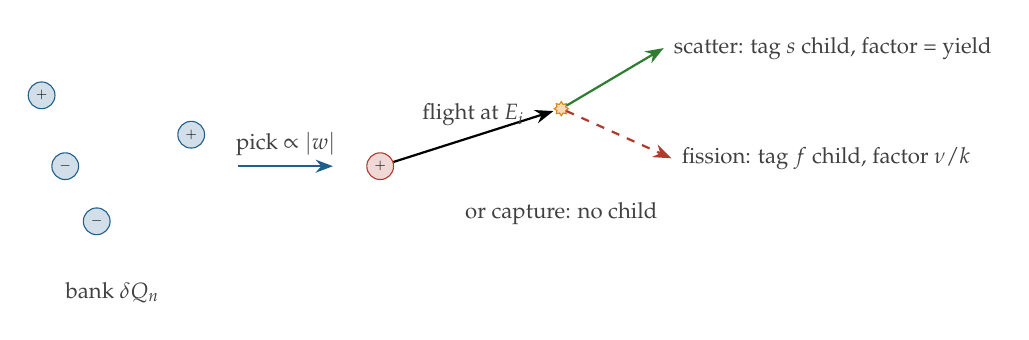
\begin{tikzpicture}[scale=1]
\foreach \x/\y/\w in {0.3/2.2/+, 1.0/0.6/-, 2.2/1.7/+, 0.6/1.3/-} {
  \node[circle,draw=\ifx\w+ accred\else headblue\fi,fill=\ifx\w+ accred!20\else headblue!20\fi,inner sep=1.5pt,font=\tiny] at (\x,\y) {$\w$};
}
\node[note] at (1.2,-0.3) {bank $\delta Q_n$};
\draw[arr] (2.8,1.3) -- (4.0,1.3) node[midway,above,note] {pick $\propto|w|$};
\node[circle,draw=accred,fill=accred!20,inner sep=1.5pt,font=\tiny] (p) at (4.6,1.3) {$+$};
\draw[-{Stealth},thick] (p) -- (6.8,2.0) node[midway,above,note] {flight at $E_i$};
\node[star,star points=8,draw=accorange,fill=accorange!30,inner sep=1.2pt] (c) at (6.9,2.03) {};
\draw[-{Stealth},thick,accgreen] (c) -- (8.2,2.8) node[right,note] {scatter: tag $s$ child, factor = yield};
\draw[-{Stealth},thick,accred,dashed] (c) -- (8.3,1.4) node[right,note] {fission: tag $f$ child, factor $\nu/k$};
\node[note] at (6.9,0.7) {or capture: no child};
\end{tikzpicture}
\caption{A forward correction flight: a parent chosen by $|w|$ flies to its next collision with
OpenMC's geometry and collides with OpenMC's physics; the child inherits the parent's sign and the
weight $\Wabs/N_\delta$ times its factor.}\label{fig:flight}
\end{figure}

OpenMC never sees a signed weight: every routine called receives a positive scratch particle of unit
weight, and the bookkeeping of signs, tags and yields stays in our code.

\section{The eigenvalue iteration}\label{sec:iteration}

With a frozen field shape a generation is (Figure~\ref{fig:overview}):
\begin{enumerate}
\item choose $b$ (fixed, or matched to the bank's per-tag mass);
\item residual records for both tags, weighted with $(a,b,k_n)$; flights of the bank;
\item cancellation (Section~\ref{sec:cancellation});
\item fission production $f_n=k_n\big(b_f\langle1,\Qmg_f\rangle+\sum_{\text{tag }f}w\big)$ and
  $k_{n+1}=k_nf_n$; never clipped, and $f\le0$ is reported as a failure of the estimator;
\item normalization: tag $s$ by $1/f_n$, tag $f$ by $k_n/(k_{n+1}f_n)$, in the bank and the field
  amplitudes, $a_{n+1}=(b_s/f_n,\;b_fk_n/(k_{n+1}f_n))$;
\item unbiased systematic resampling of the bank to at most $N_B$ sites.
\end{enumerate}
The driver sees its backend only through a dozen operations, so it is tested against a deterministic
four-region toy that iterates expected values; it reproduces the toy to $10^{-12}$.

\subsection{Amplitudes and the choice of $b$}

The field's amplitudes $a$ follow from the normalization; the amplitudes $b$ of the field candidate
kept for the next generation are a free choice made before the generation's samples, and any such
choice is unbiased. With $b=(1,1)$ the field keeps its MG shape and size and the bank carries every
difference, including a systematic mass difference between the CE and MG emissions of each tag (the CE
fission emission has mass $1/k$, the MG field's $1/k^{\mathrm{MG}}$). Per-tag \emph{mass matching}
chooses $b_t=a_t+\langle1,\delta Q_t\rangle/\langle1,\Qmg_t\rangle$ from the bank's exact signed tag
sums, so that the field absorbs the bank's net mass and the bank carries only the shape; in the toy
model it converges to the CE/MG mass ratios. It changes the bank's net weight and hence the variance,
not the mean.

\subsection{Bias of the eigenvalue estimate}

As in any Monte Carlo power iteration, normalizing each generation by an estimated $f_n$ introduces a
bias of order $1/N$ per generation in $k$ and in the source shape. It is the same mechanism as the
population-control bias of analog eigenvalue Monte Carlo and is negligible at the population sizes
used here; it is distinct from any bias of the estimators, which are unbiased given the normalization.

\section{Sign cancellation}\label{sec:cancellation}

\subsection{Why it is needed}

Each generation adds the residual's absolute weight to the bank, and flights carry most of it on in a
multiplying medium. Positive and negative particles never meet, so without cancellation $\Wabs$ grows
linearly with the generation and the noise of every tally with it (Figure~\ref{fig:s8:wabs}). The
remedy is to replace parts of the bank by particles with the same expectation and smaller absolute
weight.

\subsection{The pooling identity}

\begin{lemma}[Pooling]\label{lem:pooling}
Let a particle of weight $w$ be drawn at $y\sim p$, with $w$ independent of $y$, and let $q$ be a
density with $p>0$ wherever $q>0$. For any constant $s$,
\begin{equation}
\E[w\,\delta_y]=\E\Big[w\Big(1-s\frac{q(y)}{p(y)}\Big)\delta_y\Big]+\E\Big[w\,s\frac{q(y)}{p(y)}\Big]\,q .
\end{equation}
\end{lemma}
\begin{proof}
For any response $v$: $\E[w(1-sq/p)v(y)]=w\int(p-sq)v$ and $\E[wsq(y)/p(y)]=ws\int q=ws$, so the
right side is $w\int pv-ws\int qv+ws\int qv=w\int pv$.
\end{proof}
The particle is replaced by a \emph{kept} particle at $y$ with weight $w(1-sq/p)$, plus a
\emph{pooled} weight $wsq(y)/p(y)$ attached to a fresh draw from $q$. Pooled weights of many particles
that share the same $q$ can be added \emph{before} drawing, and there opposite signs cancel exactly.
Two remarks make it practical: a constant factor in $p$ cancels if $s$ is chosen in the same units;
and if $sq/p\approx1$ the kept weights are small, so the absolute weight drops by the cancellation
inside the pool.

\begin{figure}[t]\centering
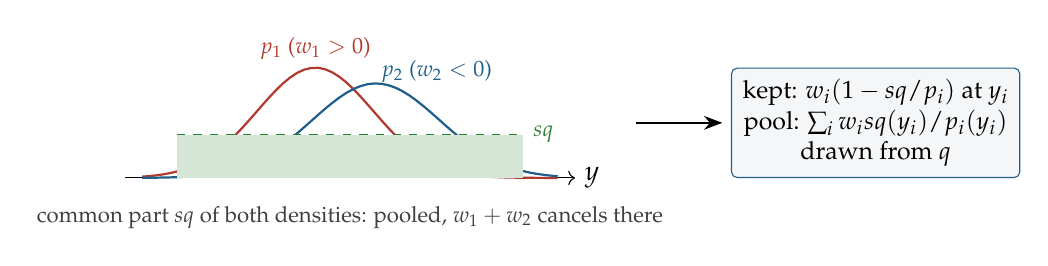
\begin{tikzpicture}[xscale=1.1]
\draw[->] (0,0) -- (5.2,0) node[right] {$y$};
\draw[thick,accred,domain=0.2:5,samples=60] plot (\x,{1.4*exp(-(\x-2.2)^2/0.9)});
\node[accred,font=\footnotesize] at (2.2,1.65) {$p_1$ ($w_1>0$)};
\draw[thick,headblue,domain=0.2:5,samples=60] plot (\x,{1.2*exp(-(\x-2.9)^2/1.1)});
\node[headblue,font=\footnotesize] at (3.6,1.35) {$p_2$ ($w_2<0$)};
\draw[thick,accgreen,dashed] (0.6,0.55) -- (4.6,0.55) node[right,font=\footnotesize] {$sq$};
\fill[accgreen!20] (0.6,0) rectangle (4.6,0.55);
\node[note] at (2.6,-0.5) {common part $sq$ of both densities: pooled, $w_1+w_2$ cancels there};
\draw[-{Stealth},thick] (5.9,0.7) -- (6.9,0.7);
\node[box,anchor=west] at (7.0,0.7) {kept: $w_i(1-sq/p_i)$ at $y_i$\\ pool: $\sum_iw_isq(y_i)/p_i(y_i)$\\ drawn from $q$};
\end{tikzpicture}
\caption{The pooling identity. Each particle's density is split into a common part $sq$ and a
remainder; the common parts of particles of opposite sign cancel exactly in the pool.}\label{fig:pooling}
\end{figure}

\subsection{Exact methods}

\textbf{Destination pooling.} With every channel of the fission residual on the sampler route, the
low-term record and the sampled fission particles of one destination share its position, and all
their directions are isotropic and independent of their weights. The low term's target density
$-b_fQ_f(\vr^\star,E)$ is known, so its \emph{whole} mass goes to the pool. A sampled fission
particle at energy $E$ came from $p=\chi_m(E\mid E')$ (its nuclide at its incident energy) and is
pooled into $q_R$, the region's lifted fission spectrum, with $s=1$. One pooled particle per
destination carries the net of the high and low terms, which is the residual there.

\textbf{Regional cancellation.} A fission child of an isotropic tag-$f$ parent at $\mathbf x_p$ with
energy $E_p$ and nuclide $m$, whose flight was shorter than $d_{max}$, has the sub-density
\begin{equation}
p(\mathbf x,E)\propto K(\mathbf x\mid\mathbf x_p,E_p)\,\chi_m(E\mid E_p),\qquad
K=\sum_{\text{images},\,d<d_{max}}\frac{e^{-\tau(\mathbf x,\mathbf x'_p;E_p)}}{4\pi d^2},
\end{equation}
the point kernel summed over the parent's mirror images in the reflective faces (each image is
reached by a reflected straight path of the same length $d$). Restricting to $d<d_{max}$ makes the
sum finite and the density exact for that event. Its weight depends only on the parent and nuclide.
The children are pooled into $q$ = uniform over the fuel pin times a reference fission spectrum, with
$s=V_{pin}\min K\,\min_E\chi_m/q_E$: the regional cancellation of Belanger, Mancusi and Zoia.

\subsection{Approximate method: binned netting}

Bins $b=(t,Z,g,d)$: tag, a zone (material times a coarse grid of the source-region mesh), group,
and for tag $s$ a direction bin. The net $m_b=\sum_{i\in b}w_i$ is re-sampled as $n_b$ particles with
$\E[n_b]=N|m_b|/\sum|m|$ and weight $m_b/\E[n_b]$: a region of the zone with probability
$V_RQ_{t,R,g}$, uniform within it, the lift in energy, uniform in the direction bin. With an
\emph{exact low term}, the records carry no low term and each bin receives
$-b_t\sum_{R\in Z}V_RQ_{t,R,g}/D$ in closed form. Binned netting keeps every bin's net in expectation;
its bias is the replacement of the within-bin shape by the field's shape, and shrinks with the bins
(at the cost of less cancellation: the region-size trade-off).

\subsection{A model of the bank's absolute weight}\label{sec:wabs}

Let $A$ be the absolute weight the residual adds each generation, $\eta$ the factor by which flights
multiply the absolute weight of a bank (production per collision, $\approx\nu\Sigma_f/(k\Sigma_t)+
\Sigma_s/\Sigma_t$, close to one in a critical, weakly leaking system), and $\kappa\le1$ the factor
that cancellation leaves. Then
\begin{equation}
W_{n+1}=\kappa\,(\eta\,W_n+A)\quad\Longrightarrow\quad
W^\ast=\frac{\kappa A}{1-\kappa\eta}\ \text{ if } \kappa\eta<1,
\end{equation}
and $W_n\approx nA$ without cancellation ($\kappa=1$, $\eta\approx1$). Two lessons follow. Any
cancellation with $\kappa<1/\eta$ makes the bank stationary, but the stationary weight is
$\kappa A/(1-\kappa\eta)$, which is large unless $\kappa$ is well below one: cancellation must remove a
substantial fraction of the weight \emph{every} generation. And $A$, the residual's absolute weight,
sets the scale: a residual estimator with production-scale noise has $A$ of the order of the production
and makes the bank as noisy as analog Monte Carlo.

\subsection{The bias of binned netting}\label{sec:netting-bias}

Netting replaces the particles of a bin by draws from the field's shape within the bin. If the
bank's true density in the bin is $\delta Q|_b$ with net $m_b$, the replacement has density
$m_b\,s_b$ with $s_b$ the field's normalized shape, so the error in a response $v$ is
$\int_b v\,(\delta Q|_b-m_b s_b)$: zero for responses constant over the bin, and first order in the
bin size times the gradient of $v$ and of the bank's shape otherwise. The error propagates through
later generations like any source perturbation, damped by the dominance ratio. Refining the bins
reduces it, at the cost of less cancellation for a fixed bank size.

\begin{keybox}[Classes of cancellation]
\begin{tabular}{@{}lll@{}}
\textbf{exact} & destination pooling & fission residual, sampler route; cancels the low term\\
 & regional (point kernel) & fission children of isotropic tag-$f$ parents\\
\textbf{approximate} & binned netting & everything; with or without the exact low term\\
\end{tabular}
\end{keybox}

\section{Correction tallies}\label{sec:tallies}

Generation $n$ reports the reaction rate of the flux its own source produces, with the same
normalization:
\begin{equation}
T_{R,n}=\frac{1}{f_n}\Big(a_{s,n}X_{s,R}+a_{f,n}X_{f,R}+\langle\Sigma_f\mathbf 1_R,\G\,\delta Q_n\rangle\Big),
\qquad X_{y,R}=\langle\Sigma_f\mathbf 1_R,\G\Qmg_y\rangle .
\end{equation}
The \textbf{field part} $X_{y,R}$ is estimated fresh each generation from backward CE traces (points
uniform in the box, one isotropic direction, $n_E$ incident energies from the region's lifted flux);
fresh points keep its error out of the long-run average. The \textbf{bank part} is a collision
estimator during the flights: each collision scores the flight's signed unit weight times
$\Sigma_f/\Sigma_t$ to its region. Both are unbiased for their terms, so $T_{R,n}$ averaged over active
generations estimates the fission rate distribution, up to the usual eigenvalue normalization bias.

\section{General properties: variance and computational complexity}\label{sec:properties}

\subsection{Cost per generation}

Let $S$ be the segments per backward trace, $n_E$ the energies evaluated per direction, $c_{tr}$ the
cost per segment of tracing and $c_{xs}$ the cost of one cross-section lookup. A residual sample
costs
\begin{equation}
C_{res}\approx J\,S\,(c_{tr}+n_E\,c_{xs})+JK\,c_{coll},
\end{equation}
with $n_E$ the number of images (one per nuclide with $A>1$) plus drawn energies, and $c_{coll}$ one
sampler-route collision. A flight costs one OpenMC flight to the next collision plus one collision; a
field-tally point costs one trace. A generation with $N$ residual samples per tag, $N_\delta$ flights
and $N_T$ tally points costs
\begin{equation}
C_{gen}=2N\,C_{res}+N_\delta C_{fl}+N_TC_{tr}+C_{canc}(N_B),
\end{equation}
where binned netting is linear in the bank size and the regional method costs one point-kernel
evaluation per eligible child (a few dozen image traces).

\subsection{Variance per generation}

The variance of a generation's estimate of a tally has three sources: the residual (whose per-sample
variance $V_{res}$ was measured in Section~\ref{sec:res:controlled}), the flights (variance proportional
to $\Wabs^2/N_\delta$), and the field part of the tally. Without cancellation $\Wabs$ grows with the
generation; with it, $\Wabs$ reaches a stationary value set by the balance between what each
generation adds ($\propto\sqrt{V_{res}/N}$ per bin) and what cancellation removes. The figure of merit
then behaves as
\begin{equation}
\mathrm{FOM}_{RMC}\propto\frac{1}{C_{gen}\,\big(V_{res}/N+\kappa\,\Wabs^2/N_\delta\big)},
\end{equation}
to be compared with analog Monte Carlo's $1/(C_{hist}V_{hist})$ per history. The method gains when the
residual is small relative to the production (small $V_{res}$) and cancellation keeps $\Wabs$ small;
it loses when either estimator noise is production-scale or the bank's absolute weight grows.

\subsection{Convergence and correlation of the emission-source iteration}\label{sec:convergence}

The iteration applies $\B$, the \emph{collision-to-collision} operator, not the fission-to-fission
operator of analog eigenvalue Monte Carlo. Its eigenvalues are those of one collision generation:
apart from the fundamental mode, which it shares with the fission source iteration, it has modes that
decay as slowly as the scattering ratio $c=\Sigma_s/\Sigma_t$ of the system, close to one in a
moderator. Two consequences follow, both measured in Section~\ref{sec:res:stage8}:
\begin{itemize}
\item \textbf{A long transient.} Starting from the converged MG field with an empty bank, the bank must
  build up the correction through these slow modes; $k_n$ approaches its limit as $c^n$. In graphite
  ($c\approx0.98$ at most energies) tens of generations are needed, so many more inactive generations
  are required than in analog eigenvalue Monte Carlo of the same problem.
\item \textbf{Strong correlation between generations.} Noise injected into the bank in one generation
  persists for about $1/(1-c)$ generations. The variance of a mean over $n$ active generations is
  $\sigma_{gen}^2\,\tau/n$ with an integrated autocorrelation time $\tau\approx(1+c)/(1-c)$, so batch
  means over short blocks underestimate the error; independent replicas measure it honestly.
\end{itemize}
Both are properties of the emission-density formulation, not of the estimators; they argue for
accelerating the slow scattering modes (e.g.\ by keeping more of each generation in the field, through
mass matching or a swept field) and for counting generations, not histories, when comparing costs.

\subsection{What scales with what}

\begin{itemize}
\item \textbf{The field's error.} Only the density route's variance falls with it (pointwise
  cancellation); the density-free route's high-term noise does not, unless the low term is cancelled.
\item \textbf{Problem size.} The residual's cost per sample depends on the trace length, which grows
  with the mean free path relative to the geometry; in large reflective problems roulette bounds it.
\item \textbf{Representation size.} Netting needs particles per bin: finer bins mean less bias and
  less cancellation for a fixed bank; the bank needed grows with the number of bins.
\end{itemize}

\part{Results}\label{part:results}

\section{Verification problems and references}\label{sec:res:setup}

\textbf{Problems.} All results use two problems built in \code{examples/rmc/problems.py}, both with
\emph{matched physics} (no unresolved-resonance probability tables, stationary target for every
nuclide with $A>1$ above $10^{-6}kT$, nearest-temperature data at 294 K), so that the elastic
evaluator is exact and the reference Monte Carlo has the same physics:
\begin{itemize}
\item \textbf{Infinite medium}: 3.1\%-enriched UO$_2$ and graphite homogenized in a reflective box,
  one source region. It has no spatial residual at all, so it isolates spectral and kinematic
  effects, and its backward flux has the closed form $q(E')/\Sigma_t(E')$.
\item \textbf{Graphite pincell}: a UO$_2$ pin (radius 0.4096 cm) in graphite, pitch 1.26 cm, height
  2 cm, reflective on every face; a $12\times12$ source-region mesh gives 172 regions. CASMO-8 groups;
  random ray with 500 rays per batch and 500 batches (300 inactive); $k^{\mathrm{MG}}=0.64257$.
  Graphite without S($\alpha,\beta$) is unphysical but a consistent CE model for both methods.
\end{itemize}
The pincell is strongly under-moderated (the pin occupies a third of the cell, and graphite needs
about 115 collisions to thermalize a neutron), so its spectrum is hard: the flux per unit lethargy
peaks near 1 MeV, fast fission in U-238 matters, and $k\approx0.64$.

\textbf{References.} Every layer is compared with something stock OpenMC computes independently: the
uncollided flux of the field as a fixed source (\code{CollisionFilter([0])}), first-collision
production (\code{CollisionFilter([1])} in one-batch eigenvalue runs, so that fission neutrons are
banked rather than transported), flights from the field's own weighted sample, and finally OpenMC's
eigenvalue calculation. Appendix~\ref{app:gates} lists the gates.

\section{Components}\label{sec:res:components}

\subsection{The field and the backward flux}

\begin{figure}[t]\centering
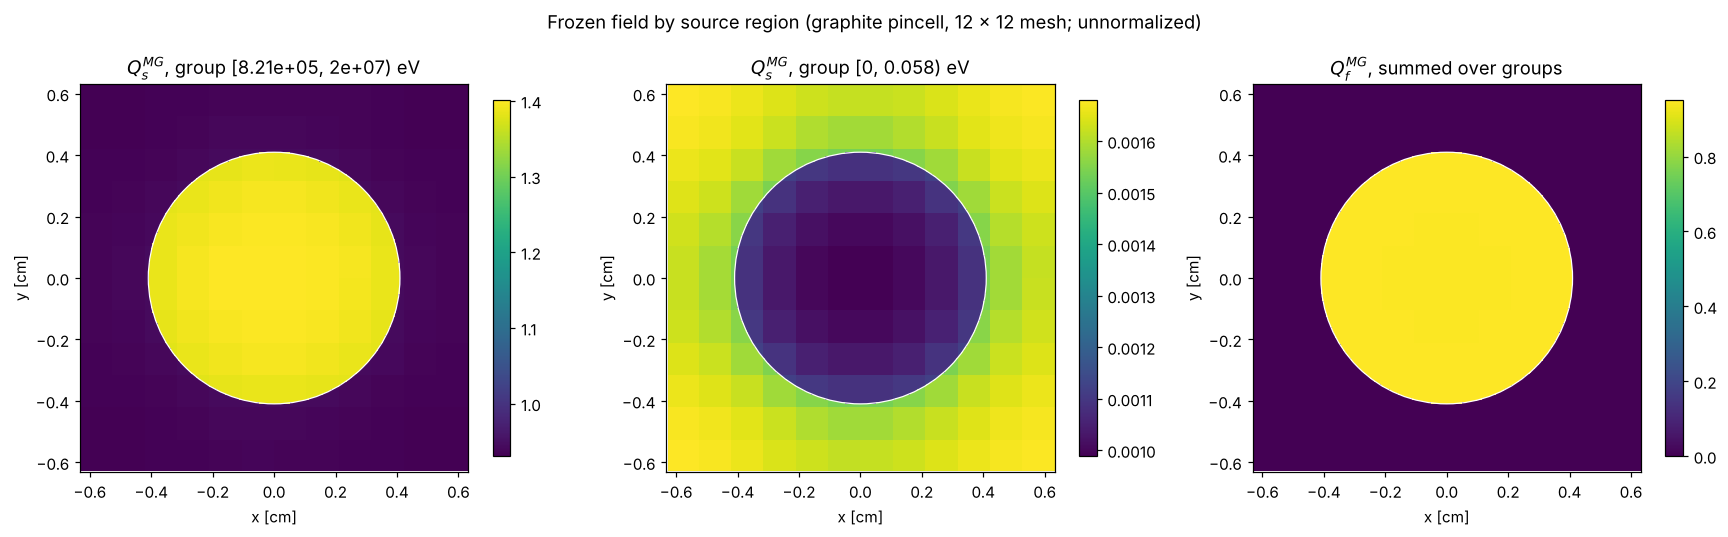
\includegraphics[width=\textwidth]{figures/field_maps.png}
\caption{The pincell's field: MG emission by region for both tags and a few groups. Fission emission is
confined to the fuel; scattering emission is largest in the graphite at low energy and in the fuel at
high energy.}\label{fig:res:field}
\end{figure}

\begin{figure}[t]\centering
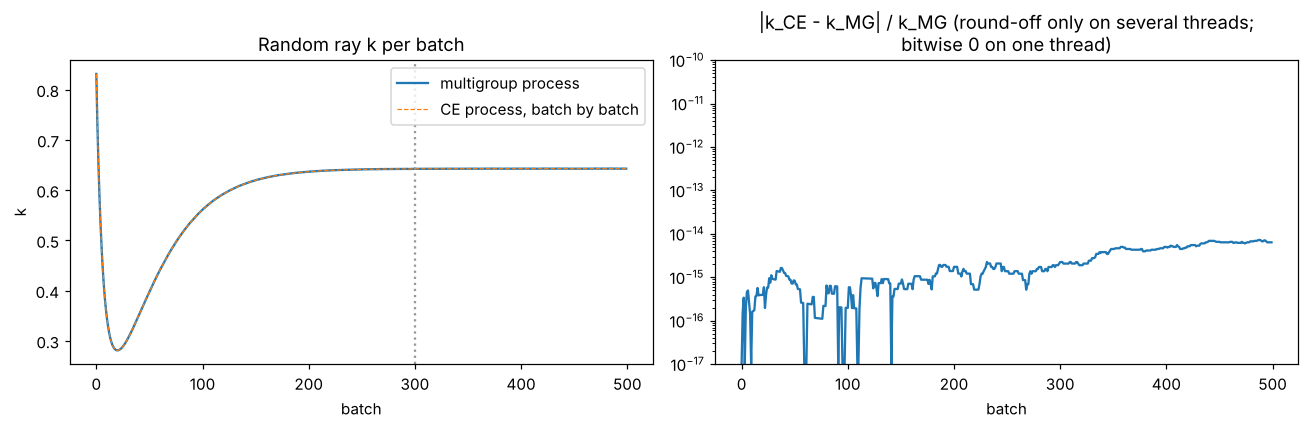
\includegraphics[width=\textwidth]{figures/ce_vs_mg.png}
\caption{CE against MG backward flux on identical paths. The two agree where the MG cross sections
represent the CE ones (smooth ranges) and differ inside resonance groups, where one MG $\Sigma_t$
averages a factor of $10^3$ of variation: this difference is what the MG control cannot remove.}\label{fig:res:cevsmg}
\end{figure}

Figure~\ref{fig:res:cevsmg} is the key picture for the control variate. Along a single path the MG
and CE fluxes share the geometry and the source, and differ only through the cross sections. In
groups where the CE cross section varies little the two fluxes are almost identical, so the MG flux
removes the path's directional noise. In the resonance group (4 eV to 5.53 keV) the CE flux depends
on the exact energy relative to the U-238 resonances, and no single group constant follows it.

\begin{figure}[t]\centering
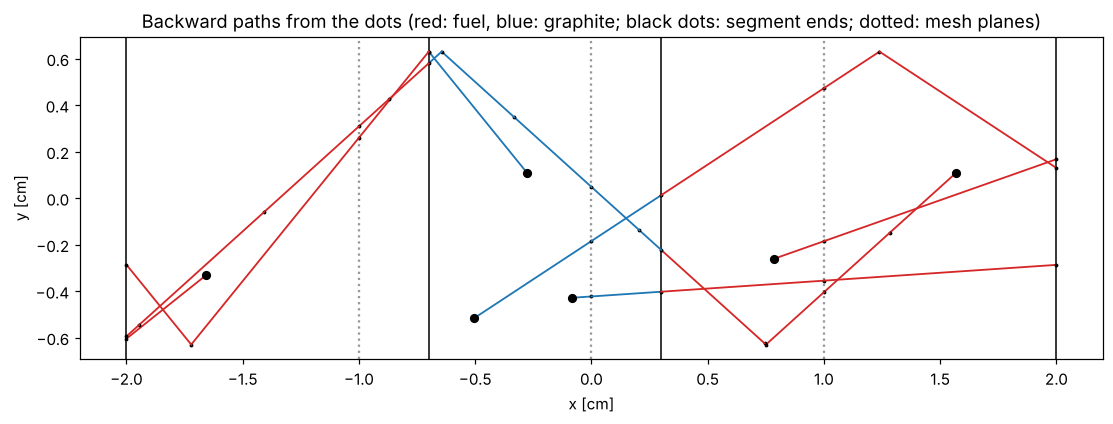
\includegraphics[width=\textwidth]{figures/tracer.png}
\caption{Backward traces through the pincell's source-region mesh and reflective faces, coloured by
region, against the analytic unfolded paths (G2.1): the tracer reproduces lengths, materials and
regions to $10^{-10}$ cm.}\label{fig:res:tracer}
\end{figure}

\subsection{Residual against first-collision tallies}

\begin{figure}[t]\centering
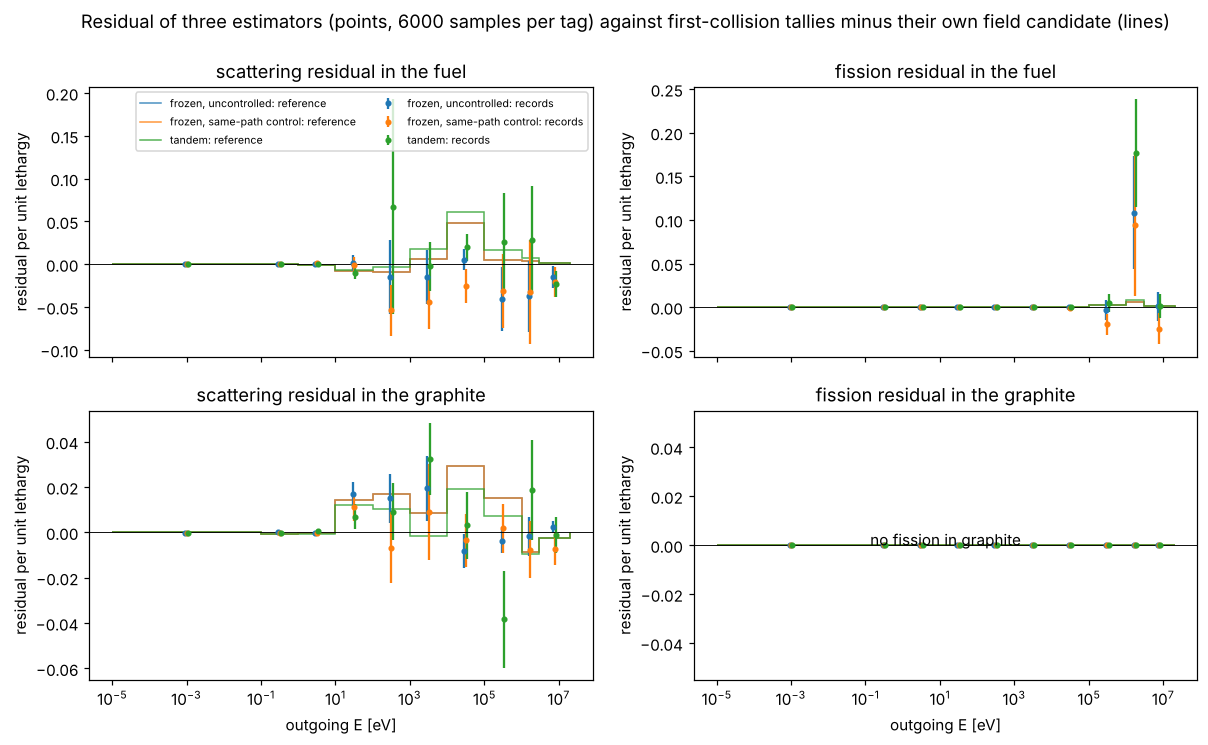
\includegraphics[width=\textwidth]{figures/first_collision.png}
\caption{The residual of the pincell's field by material and outgoing energy: OpenMC's first-collision
production minus the field integrated exactly (black) against several estimators (G4.1, G4.2). All
agree within statistics; their error bars differ by orders of magnitude.}\label{fig:res:fc}
\end{figure}

The residual is small: a few per cent of the production in any bin, largest in the fuel's epithermal
range (resonances) and in the fission spectrum (Figure~\ref{fig:res:fc}). Every estimator of
Table~\ref{tab:family} passes this gate, as do the density-free variants.

\section{The controlled residual study}\label{sec:res:controlled}

\subsection{Setup}

On the pincell with prescribed exact volumes, ten variants (Section~\ref{sec:classes}) were run with
$N=40{,}000$ samples per tag and compared, bin by bin, with a reference residual built from
$2.4\times10^7$ forward flights of each field component (a uniform point, a group in proportion to
the region's emission, a log-uniform energy within the group, weighted by $4\pi V\,q/p$), minus the
field integrated exactly. Three binnings: 36 logarithmic outgoing-energy bins per material; the 172
regions; and the radial cosine $\mu_\rho=\vO\cdot\mathbf e_\rho$ of the outgoing direction in each
material and energy range. Scans of $K$, common numbers, $J$, $M_{II}$ and the roulette cutoff used
$N=10{,}000$. All variants share their destination stream.

\subsection{The residual in energy, space and angle}

\begin{figure}[p]\centering
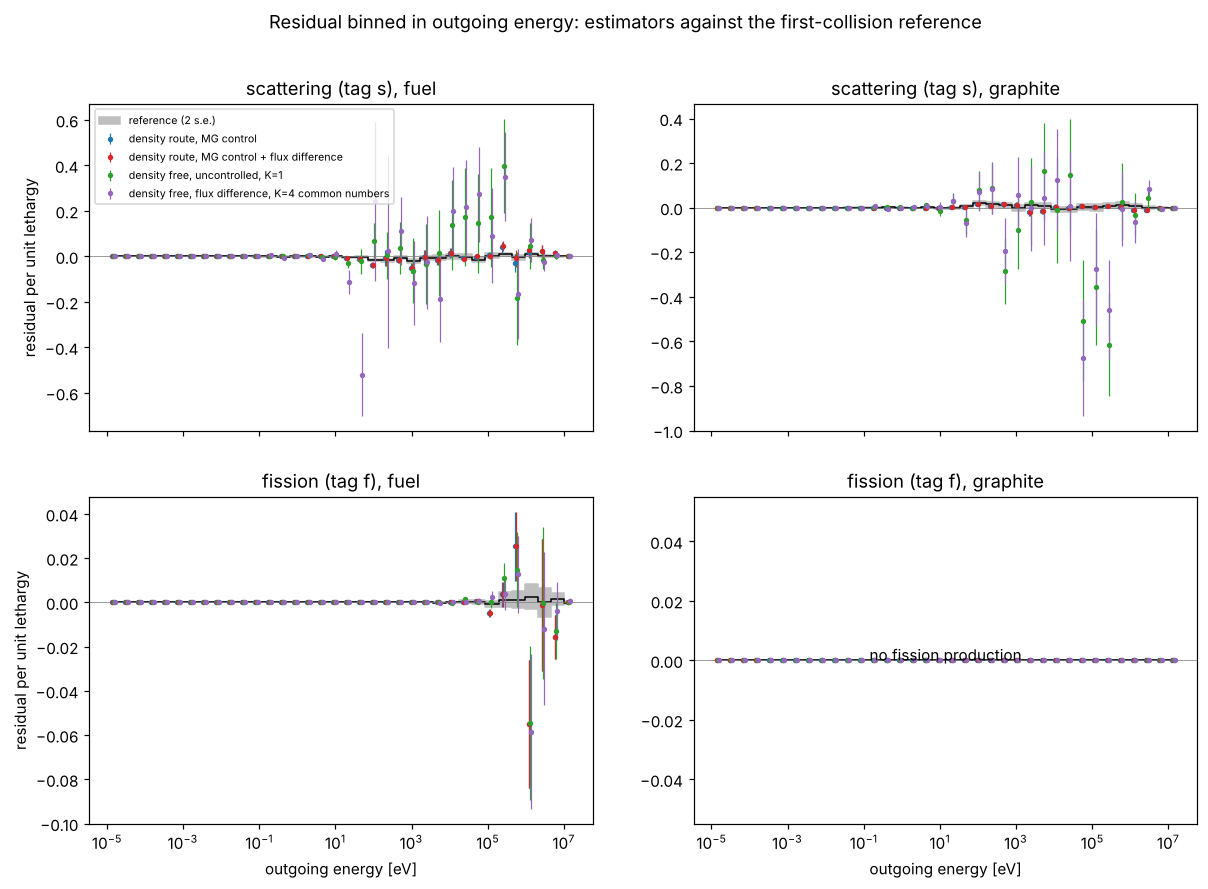
\includegraphics[width=\textwidth]{figures/controlled_energy.png}
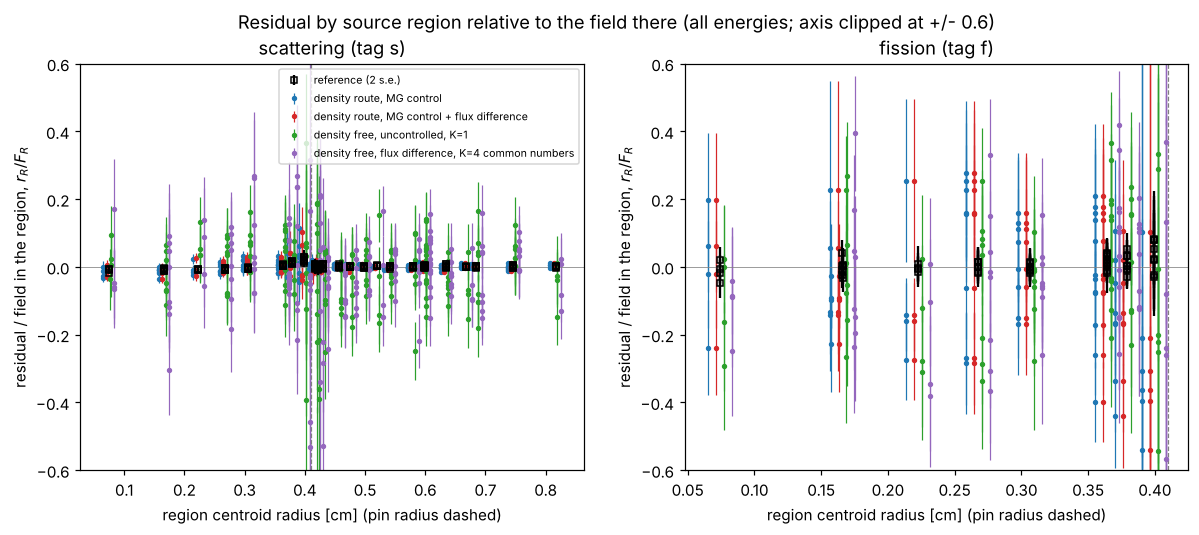
\includegraphics[width=\textwidth]{figures/controlled_space.png}
\caption{Top: residual per unit lethargy. Bottom: residual by region relative to the field there, against
the region's centroid radius.}\label{fig:res:energy}
\end{figure}

\textbf{Energy} (Figure~\ref{fig:res:energy}, top). In the fuel the scattering residual is negative
just below 4 eV and changes sign through the resonance group: the 8-group field spreads emission
uniformly in lethargy within a group as weighted by an infinite-medium-like spectrum, while the true
emission in the pin dips at every U-238 resonance (fewer neutrons there to scatter) and rises
between them. The fission residual lives between 100 keV and 10 MeV, where it reflects the difference
between the CE fission spectrum of the actual incident spectrum and the one group-collapsed $\chi$
of the MG data.

\textbf{Space} (Figure~\ref{fig:res:energy}, bottom). The reference residual is within $\pm3$\% of the
field everywhere except the small regions cut by the pin surface, where it reaches $\pm15$\%: the
field is flat within a region while the true emission has a gradient across the fuel--moderator
interface. The density route resolves these; the density-free estimators do not at this sample
size.

\begin{figure}[t]\centering
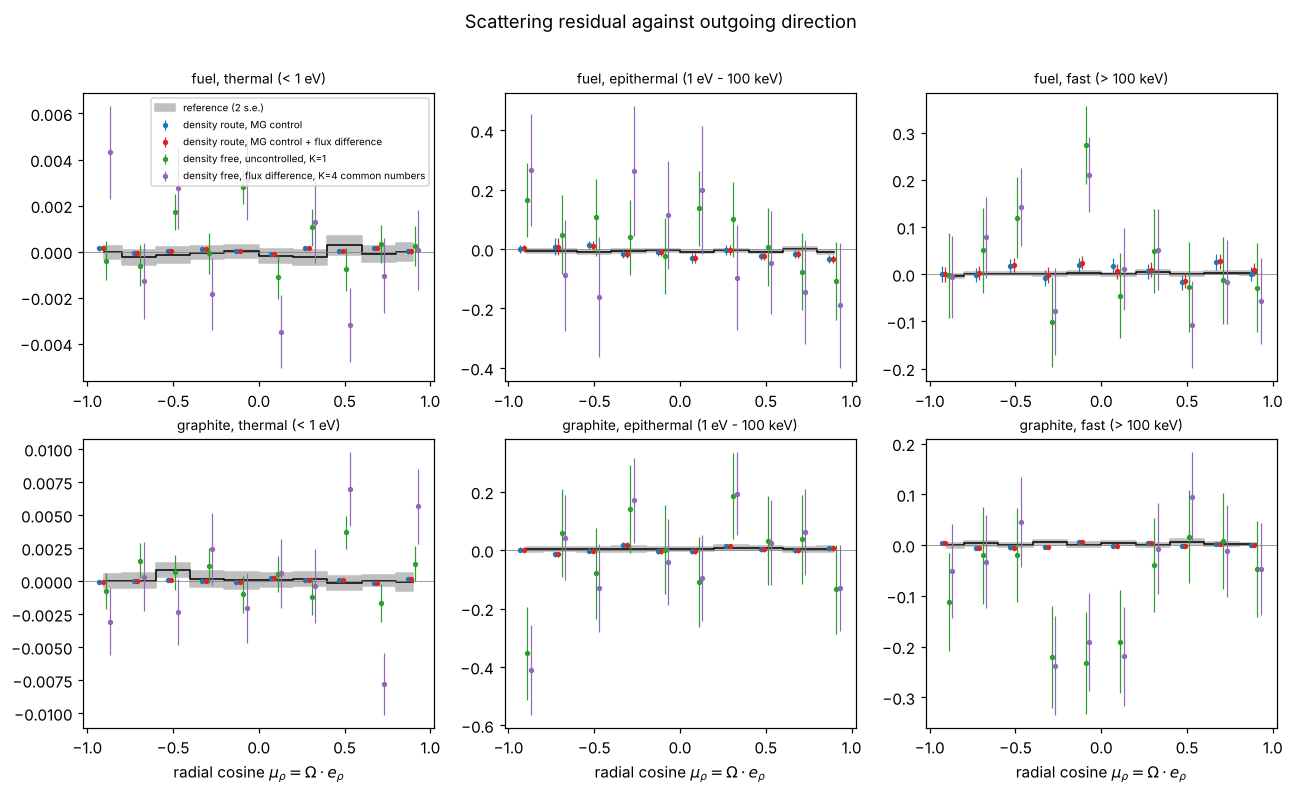
\includegraphics[width=\textwidth]{figures/controlled_angle.png}
\caption{Scattering residual against the radial cosine of the outgoing direction.}\label{fig:res:angle}
\end{figure}

\textbf{Angle} (Figure~\ref{fig:res:angle}). The field is isotropic; any angular residual comes from the
anisotropy of real scattering (forward-peaked in the lab, especially in graphite at MeV energies) and
of the flux near the pin surface. At this resolution the reference resolves no angular structure, so
this binning tests the estimators' directional noise.

\subsection{Where the variance comes from}

\begin{figure}[t]\centering
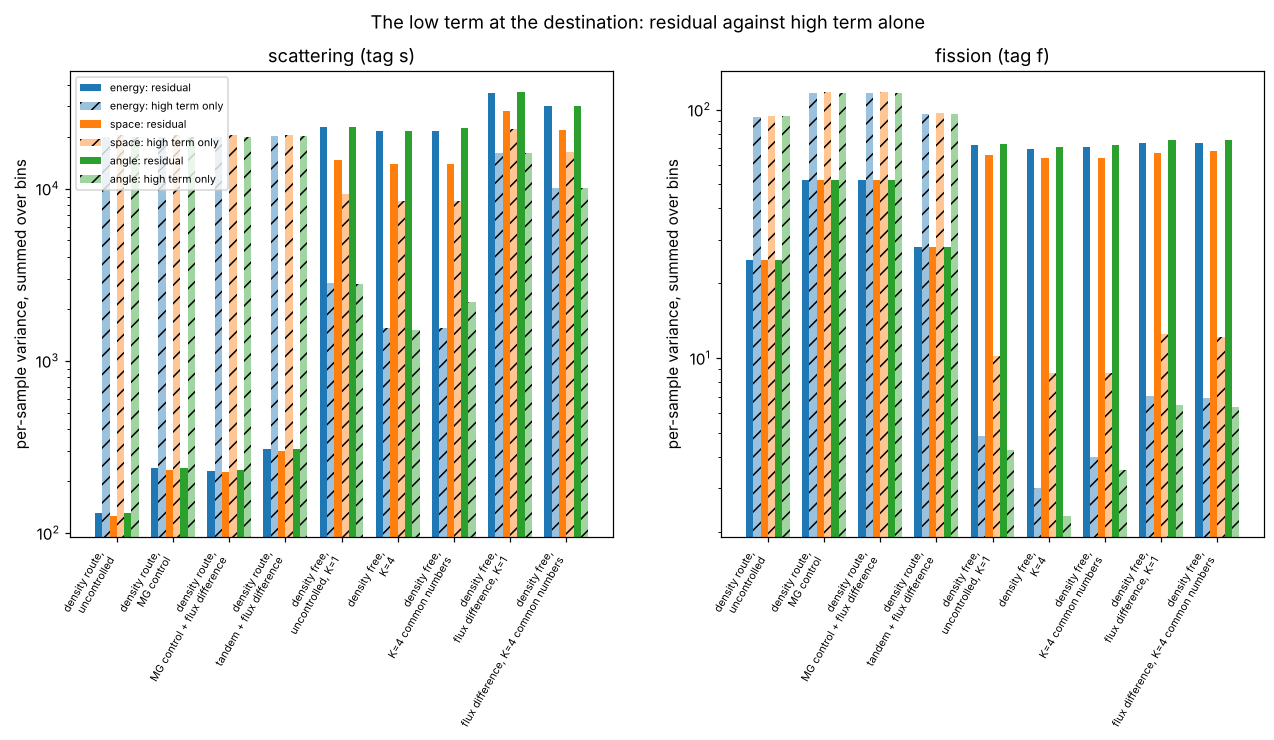
\includegraphics[width=\textwidth]{figures/controlled_low_term.png}
\caption{Per-sample variance of the residual (solid) and of the high term alone (hatched), per
binning.}\label{fig:res:lowterm}
\end{figure}

\begin{table}[t]\centering\small
\begin{tabular}{lrrrr}
\toprule
Variant & $s$: residual & $s$: high only & $f$: residual & $f$: high only\\
\midrule
density route, uncontrolled & \textbf{130} & 19{,}900 & \textbf{24.7} & 93.7\\
density route, MG control & 238 & 20{,}000 & 52.1 & 117\\
density route, tandem + flux difference & 308 & 20{,}100 & 27.9 & 95.8\\
density free, uncontrolled, $K=1$ & 22{,}800 & 2{,}840 & 72.0 & 4.86\\
density free, $K=4$ & 21{,}500 & 1{,}560 & 69.7 & 3.00\\
density free, flux difference, $K=1$ & 35{,}900 & 16{,}000 & 73.7 & 7.07\\
density free, flux difference, $K=4$ c.n. & 30{,}100 & 10{,}100 & 73.6 & 6.92\\
\bottomrule
\end{tabular}
\caption{Per-sample variance summed over the 72 energy bins.}\label{tab:res:var}
\end{table}

Three findings (Figure~\ref{fig:res:lowterm}, Table~\ref{tab:res:var}):
\begin{enumerate}
\item \textbf{Pointwise cancellation is the density route's whole advantage.} Its high term alone is
  the noisiest of all ($2\times10^4$ for scattering): the elastic image densities are large when the
  image falls on a resonance or the laboratory Jacobian is large. At the destination's state the low
  term removes 99.3\% of it.
\item \textbf{The density-free residual is dominated by the low term}: $2.05\times10^4$ of the
  scattering variance and 69 of the fission variance are the field's own integral estimated by Monte
  Carlo.
\item \textbf{The sampled high term is good}: 7 (scattering) to 19 (fission) times quieter than the
  evaluators' at $K=1$, 33 to 56 times at $K=16$.
\end{enumerate}

\begin{figure}[t]\centering
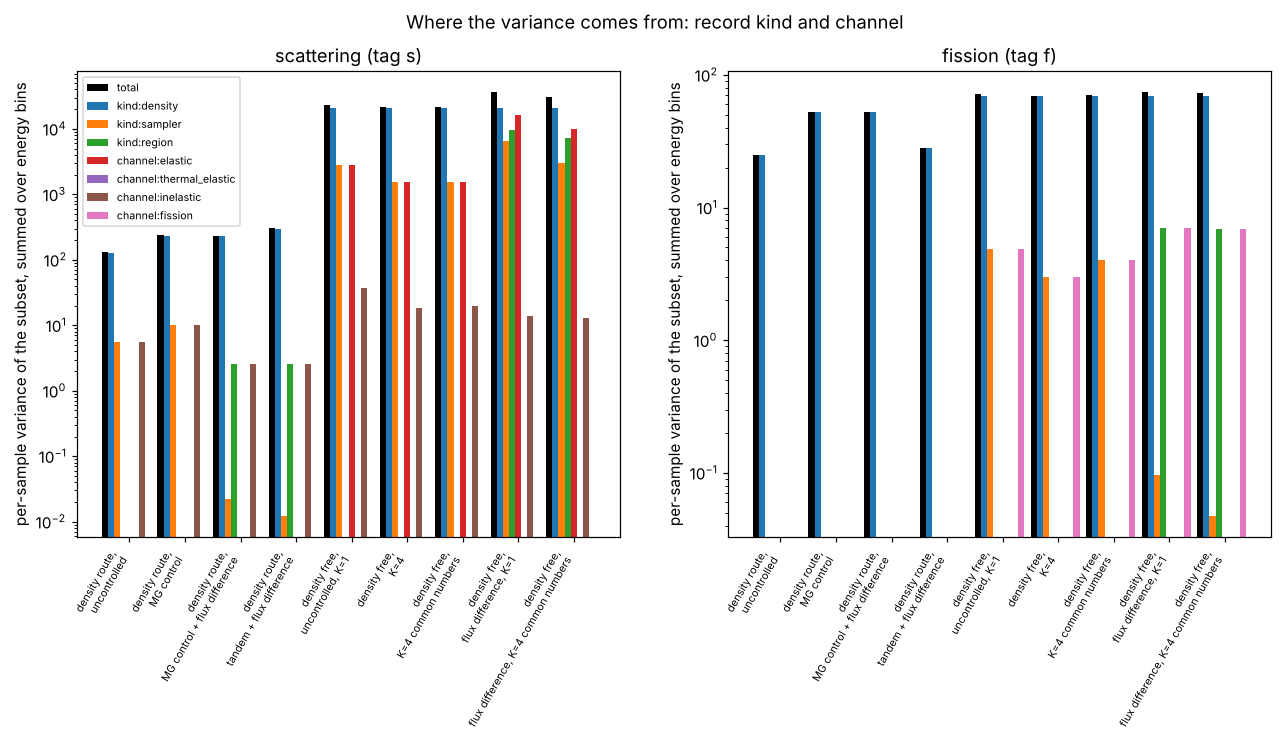
\includegraphics[width=\textwidth]{figures/controlled_decomposition.png}
\caption{Variance of the records of each kind (density branch, sampler particles on a path, region-term
particles) and channel. In every density-free variant the density branch, which then carries only the
low term, dominates; among scattering channels elastic carries almost all of the sampled variance.}\label{fig:res:decomp}
\end{figure}

\begin{figure}[t]\centering
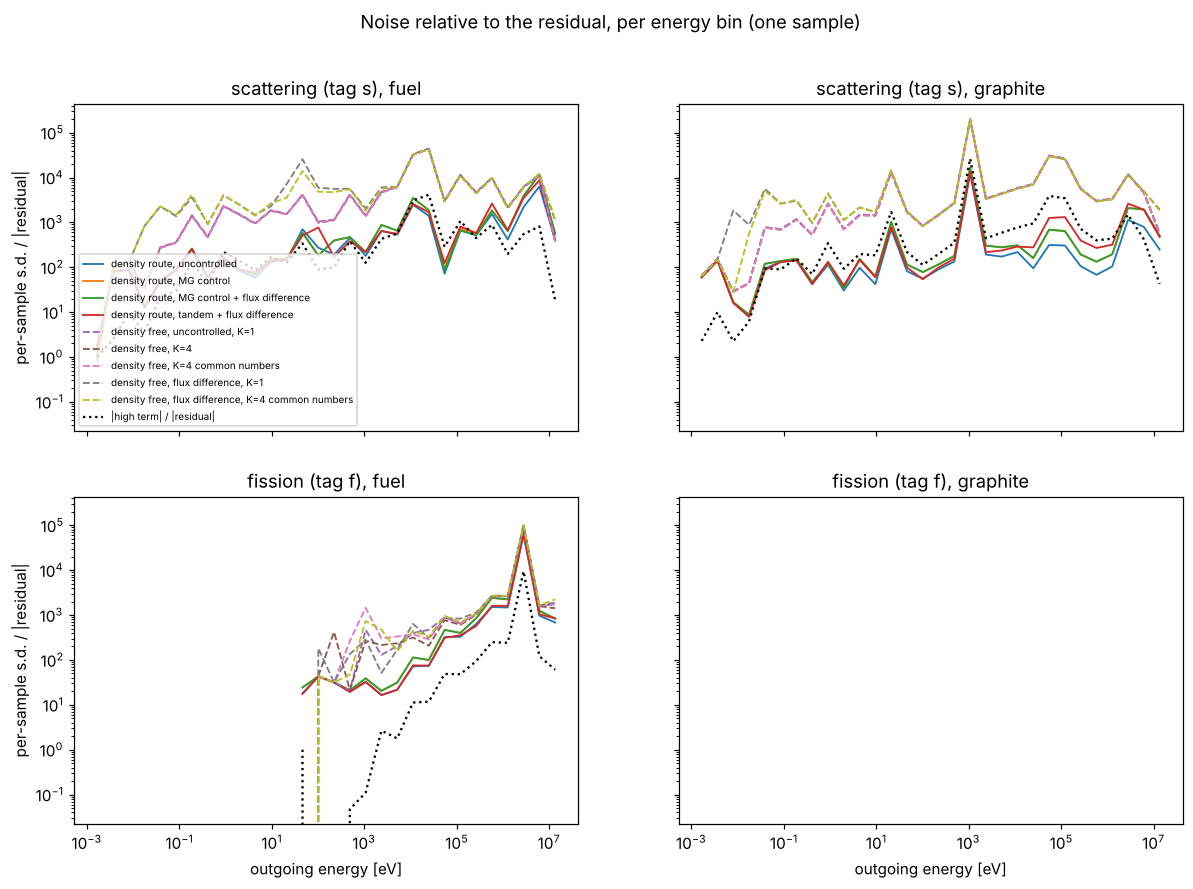
\includegraphics[width=\textwidth]{figures/controlled_relative_noise.png}
\caption{Per-sample standard deviation over $|r|$ per energy bin. The dotted line is the ratio of the
production to the residual: an estimator with production-scale noise sits on or above it. The density
route sits a factor of 3--30 below it, the density-free route on it.}\label{fig:res:relnoise}
\end{figure}

\subsection{Parameters}

\begin{figure}[t]\centering
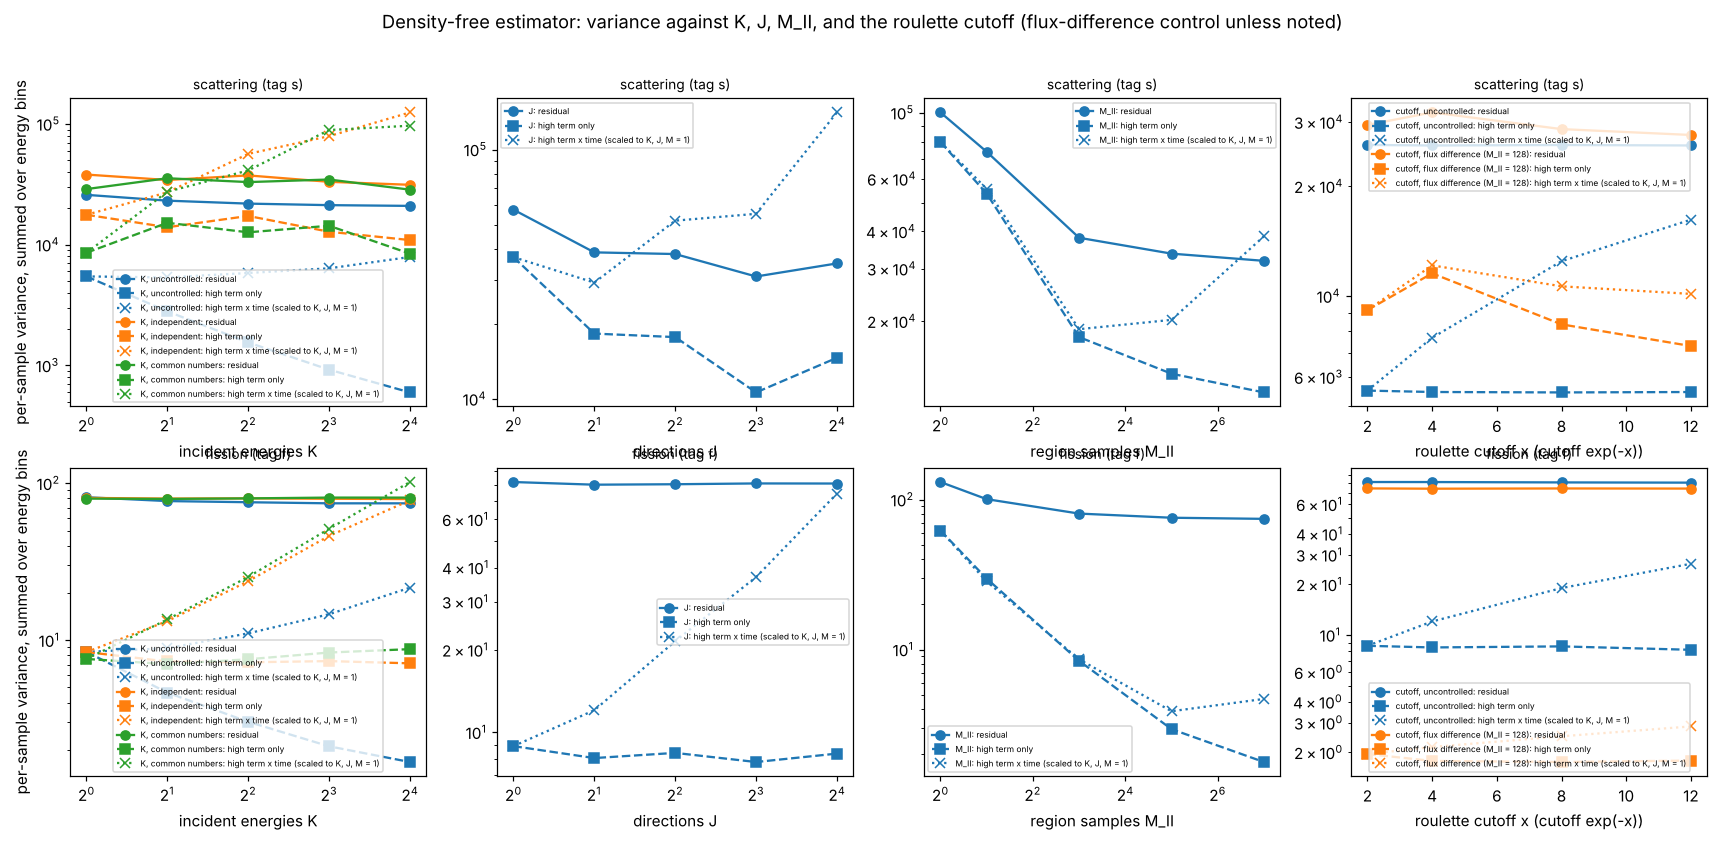
\includegraphics[width=\textwidth]{figures/controlled_scans.png}
\caption{Density-free scans: variance of the residual (circles) and of the high term alone (squares)
against $K$, $J$, $M_{II}$ and the roulette cutoff; crosses: high term $\times$ time.}\label{fig:res:scans}
\end{figure}

Figure~\ref{fig:res:scans}: more incident energies help roughly as $K^{-0.8}$, but each costs a
collision sample, so variance $\times$ time is flat; more directions help with diminishing returns;
the region term of the flux-difference control falls as $1/M_{II}$ to a floor set by term I; the
roulette cutoff hardly matters. For fission the flux-difference control works (high-term variance 1.8
at $M_{II}=128$ against 8.4 uncontrolled): the fission spectrum barely depends on $E'$, so the region's
isotropic MG flux captures the incident integral. For scattering it hurts: the isotropic,
region-averaged lifted flux is a poor match to $\psi(E')$ on a path through the pin's resonances.

\subsection{Does the noise scale with the residual?}

\begin{figure}[t]\centering
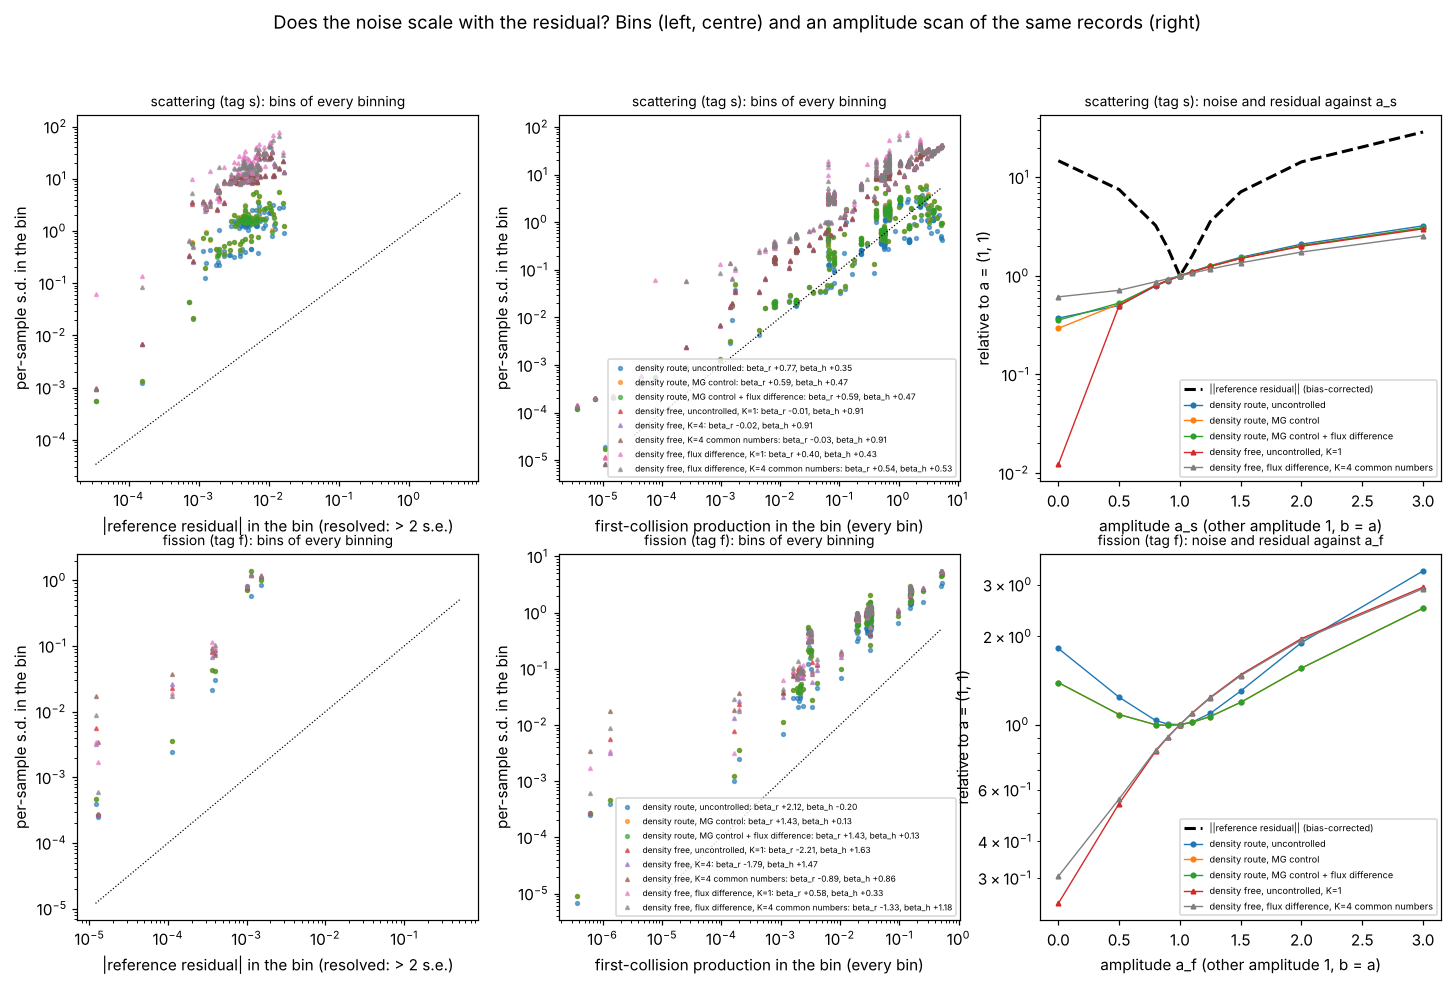
\includegraphics[width=\textwidth]{figures/controlled_noise_scaling.png}
\caption{Left, centre: per-sample standard deviation per bin against the reference residual and the
production. Right: the same records reweighted for other amplitudes, where the residual's norm grows
10 to 400 times.}\label{fig:res:scaling}
\end{figure}

Fitting $\log\sigma=\alpha+\beta_r\log|r|+\beta_h\log h$ over resolved scattering bins, the density
route has $\beta_r\approx0.5$--$0.8$ through its pointwise cancellation while every uncontrolled
density-free variant has $\beta_r\approx0$, $\beta_h\approx0.9$: production-scale noise. The amplitude
scan (Figure~\ref{fig:res:scaling}, right) asks the sharper question: when the residual grows 10 to
400 times, the noise of every estimator changes by at most 3 times, in proportion to the high term.
At the converged field no member of the family has noise that falls with the residual; what remains
is the integration noise of the high term over $\vO'$ and $E'$.

\begin{figure}[t]\centering
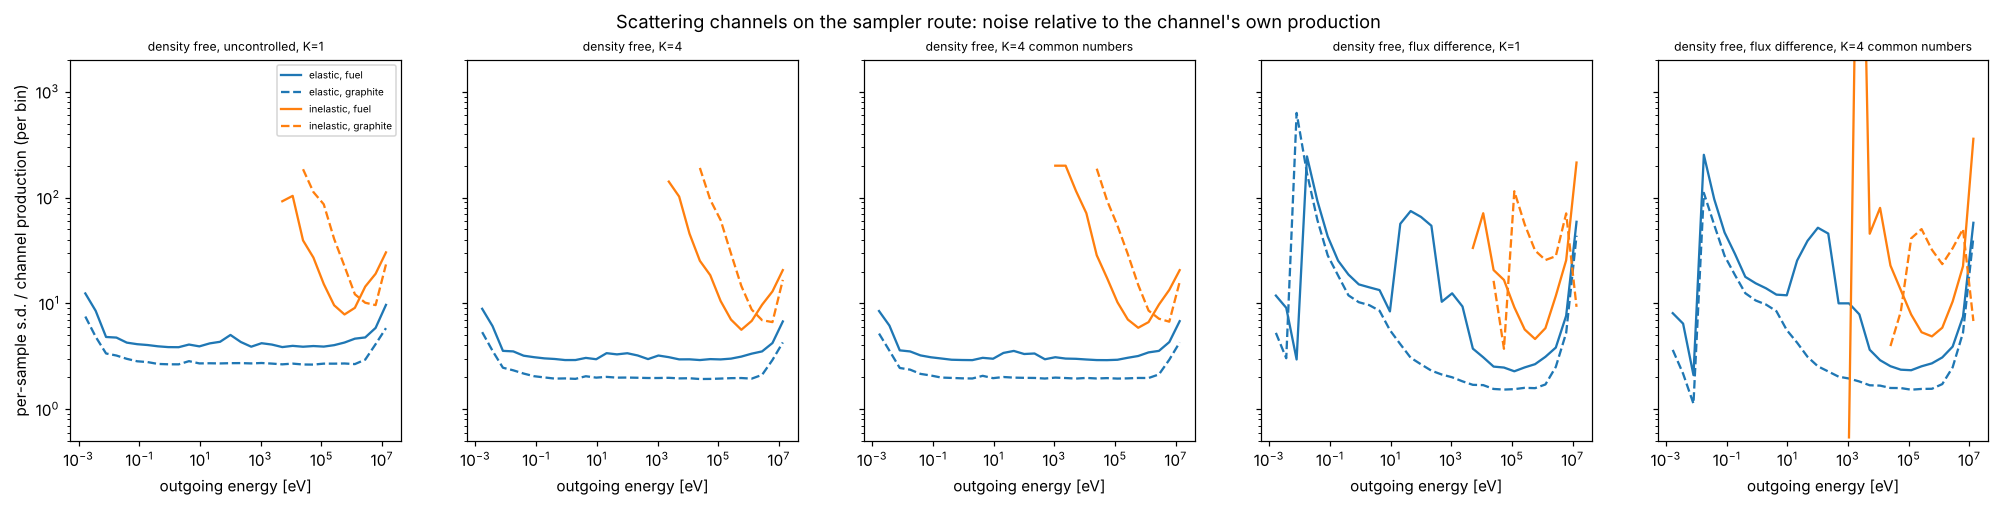
\includegraphics[width=\textwidth]{figures/controlled_channels.png}
\caption{Per-channel noise relative to the channel's own production on the sampler route: elastic about
3--4 per sample per bin, inelastic 10--100 (its production is small and sharply thresholded). The
flux-difference control lowers the elastic noise above 100 keV, where the flux is nearly isotropic and
smooth, and raises it in the resonance range.}\label{fig:res:channels}
\end{figure}

\begin{figure}[t]\centering
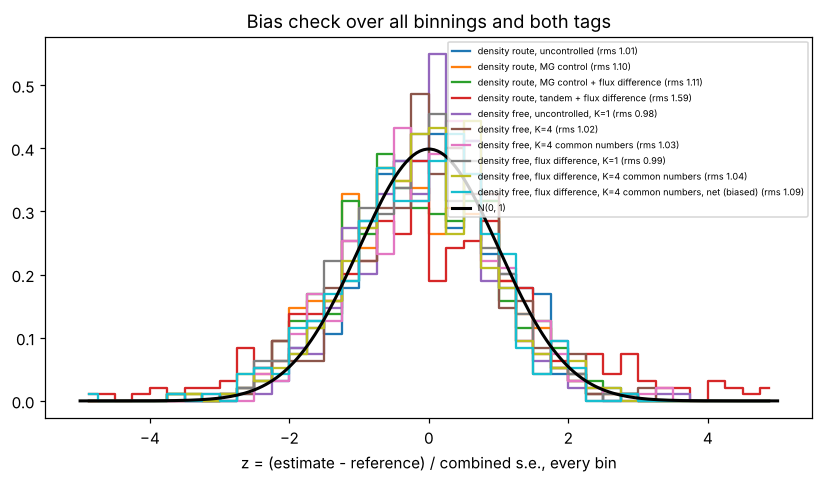
\includegraphics[width=0.85\textwidth]{figures/controlled_z.png}
\caption{Bias check: standardized differences from the reference over every resolved bin of the three
binnings and both tags. Unbiased variants follow the normal density; the net assignment (biased by
construction) is wider.}\label{fig:res:z}
\end{figure}

\subsection{The low term made exact}

With the low term exact (in a tally, or in netting bins), the efficiency (variance $\times$ time,
energy binning) is: scattering, density route 90 against 680--880 density-free; fission, density route
2.0 against 0.19--0.36 density-free. Each route should be used for what it is good at: the density
route for channels with an evaluator and pointwise cancellation, the sampler route with an exact low
term for fission and for channels without densities.

\section{The first end-to-end measurement}\label{sec:res:stage8}

% Stage 8: the first end-to-end measurement. Numbers from
% examples/rmc/stage8_analysis.py on the runs in examples/rmc/results/stage8.

\newcommand{\refk}{0.64202}
\newcommand{\refksd}{0.00049}
\newcommand{\refT}{151}


This section reports the first run of the whole method: the MG field, the residual for both tags, the
cancellers of Section~\ref{sec:cancellation}, the flights, and the correction tally. All of it ran
together on the graphite pincell and was compared with OpenMC's continuous-energy eigenvalue
calculation of the same model. The question is whether the method works at all: whether it is
unbiased, how its variance per particle and per second compares with analog Monte Carlo, and what
engineering could recover. It is not yet the question of whether it wins.

\subsection{Setup}

\paragraph{Problem.} The graphite-moderated UO$_2$ pincell of Section~\ref{sec:res:setup} has fuel
pin, gap and graphite block, reflective on every face, at 294~K with ENDF/B-VIII.0 data. Its
infinite-lattice multiplication factor is $k\approx0.642$. It is far from critical because the
moderator-to-fuel ratio is far from optimal: thermal absorption in the large graphite block competes
with the fuel.

The spectrum is strongly thermal. Fission neutrons born near 2~MeV need about 115 collisions with
carbon ($\xi\approx0.158$) to reach thermal energies. Most of those collisions happen in the
graphite, far from the pin, so the slowing-down source near the fuel is close to the
$1/E$ asymptotic form, apart from the dips at the $^{238}$U resonances. This has two consequences.
\begin{itemize}
\item Most fissions are induced by thermal neutrons that entered the pin from the moderator. The
  fission source is peaked at the pin surface and depressed at its centre: the thermal flux dips
  inside the absorbing pin.
\item The scattering ratio $c$ is close to one almost everywhere. That makes the emission-source
  iteration of Section~\ref{sec:convergence} slow and its generations strongly correlated.
\end{itemize}

\paragraph{Field.} The MG field is the 8-group flat-source random-ray solution, with prescribed
(exact) region volumes. It has 172 regions: the cells cut by the $12\times12$ source-region mesh. Of
these, 60 are fuel regions. The field eigenvalue is $k_{MG}=0.64257$, already within $55$~pcm of
the CE reference. The MG answer is close, and the correction only has to supply the fine-energy and
angular structure that 8 groups cannot represent.

\paragraph{Reference.} OpenMC eigenvalue runs, single-threaded:
\begin{itemize}
\item 4 independent replicas;
\item each with $2\times10^4$ particles per batch, 20 inactive and 50 active batches ($10^6$ active histories);
\item fission and $\nu$-fission tallied on the same fuel regions.
\end{itemize}
The results:
\begin{itemize}
\item $k=\refk\pm\refksd$ (the spread of the replicas; each replica's own batch estimate is $0.00058$);
\item $\refT$~s of active time per replica.
\end{itemize}

\paragraph{RMC runs.} \code{examples/rmc/stage8.py} runs each variant in 3 independent replicas. Two
campaigns were run:
\begin{itemize}
\item \textbf{First campaign.} 5 inactive and 30 active generations, $N_s=N_f=2000$ residual samples,
  a bank resampled to $N_\delta=2\times10^4$, $N_B=2\times10^4$ netting particles, and a CE
  correction tally with $2\times10^4$ backward points per generation.
\item \textbf{Tuned campaign} (combined variants only). 40 inactive and 60 active generations,
  $N_\delta=2\times10^5$, $N_B=4\times10^4$, and a correction tally with $10^4$ points plus the MG
  control (a one-off low tally of $4\times10^5$ points, Section~\ref{sec:tallies}). This campaign
  tallies $\nu$-fission.
\end{itemize}
Every replica is single-threaded. The figures of merit use active time only, on both sides.

\paragraph{Variants.} These are the classes of Section~\ref{sec:cancellation}:
\begin{center}\small
\begin{tabular}{@{}lll@{}}
\toprule
variant & residual routes & cancellation \\
\midrule
none & density route, both tags & none \\
binned netting & density route, both tags & netting (zones $3\times3$ per material, group bins) \\
binned, exact low (f) & s density, f sampler & netting, fission low term in closed form per bin\\
exact only & s density, f sampler & destination pooling + regional point kernel \\
exact + binned netting & s density, f sampler & pooling + regional + netting \\
exact + finer netting & as above & netting with $12\times12$ zones and 4 sub-bins per group \\
\bottomrule
\end{tabular}
\end{center}

\subsection{Stability: the absolute weight of the bank}

\begin{figure}[t]\centering
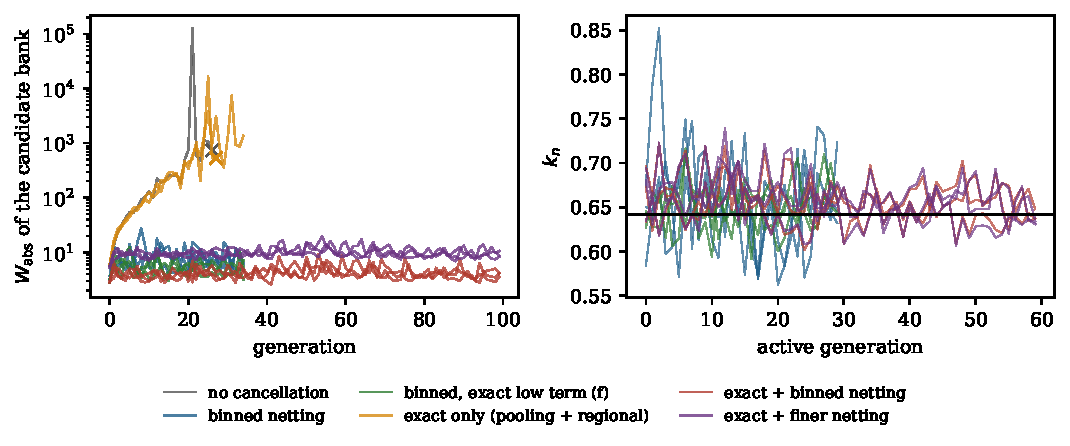
\includegraphics[width=\textwidth]{figures/stage8_wabs_k.pdf}
\caption{Left: absolute weight $\Wabs$ of the candidate bank (after cancellation) against generation,
for every variant and replica. A cross marks an estimator failure: the fission production $f$ turned
negative and the eigenvalue update became undefined. Right: the generation estimate $k_n$ over the
active generations of the variants that ran to completion, against the CE reference (black line).}
\label{fig:s8:wabs}
\end{figure}

Figure~\ref{fig:s8:wabs} answers the first question: without cancellation the method does not run.
\begin{itemize}
\item \textbf{No cancellation.} $\Wabs$ grows geometrically, by about $30\%$ per generation. Generation
  27 fails with $\Wabs\approx735$: the signed bank's noise exceeded the production it corrects and
  $f<0$. This is the instability of Section~\ref{sec:wabs}: with $\kappa\eta>1$ no stationary $\Wabs$
  exists.
\item \textbf{Exact methods alone.} Destination pooling and the regional kernel do not stop the
  growth. Pooling cancels the fission residual very well: $\Wabs$ of the fission records falls from
  $2.8$ to $0.75$ per generation. But scattering carries most of the absolute weight, and only
  netting touches it. One replica failed at generation 28, the other reached $\Wabs\approx1360$.
\item \textbf{Netting.} Every variant with netting is stable, with $\Wabs$ between 4 and 10:
  \begin{itemize}
  \item the coarse representation ($3\times3$ zones) holds $\Wabs\approx4$--$8$;
  \item adding the exact fission methods lowers it to $\approx4.4$;
  \item the finer representation, counter-intuitively, raises it to $\approx10$. More bins means
    fewer particles of opposite sign per bin, so there is less to cancel. This is the trade-off of
    Section~\ref{sec:netting-bias}: a finer representation has less bias but cancels less.
  \end{itemize}
\end{itemize}
In the tuned combined run, one typical generation looks like this:
\begin{itemize}
\item netting reduces $\Wabs$ from $11.2$ to $4.8$ over 645 occupied bins;
\item pooling moves $\approx700$ fission records into the pools and cuts their absolute weight by a
  factor $3.8$;
\item the regional kernel is eligible for only $\approx20$ of $\approx1300$ fission children.
\end{itemize}
The regional kernel acts so rarely because fission children come almost entirely from tag-s parents.
These are thermal neutrons arriving from the graphite, not the tag-f parents near the pin that the
kernel requires. In this problem it is inert, and its cost buys nothing.

\begin{figure}[t]\centering
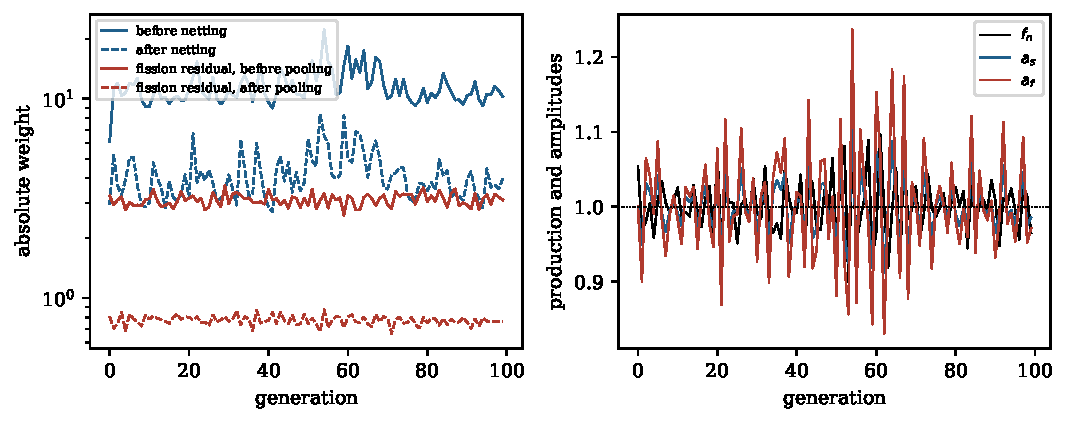
\includegraphics[width=\textwidth]{figures/stage8_diagnostics.pdf}
\caption{One replica of the tuned combined variant, generation by generation. Left: absolute weight
before and after netting (whole candidate bank), and of the fission residual before and after
destination pooling. Right: the production $f_n$ and the amplitudes $a_s$, $a_f$. Netting removes
about half of the bank's absolute weight every generation; pooling removes three quarters of the
fission residual's. The production fluctuates by about 4\% and the fission amplitude by about 8\%:
this noise, fed back through the iteration, is the leading candidate for the eigenvalue bias.}
\label{fig:s8:diag}
\end{figure}

Figure~\ref{fig:s8:diag} shows the stationary state. What remains after netting is about four times
the absolute weight of the fission residual after pooling. The scattering residual and its children,
which only netting touches, carry the variance.

\subsection{Bias}

\begin{table}[t]\centering\small
\caption{End-to-end results against the CE reference ($k=\refk$). The columns are:
$\Delta k$, the bias in pcm; $z_{bm}$ and $z_{rep}$, the bias in units of its standard error from
5-generation batch means and from the spread of the 3 replicas; $\overline{\Wabs}$, over active
generations; $T$, the active time per replica in seconds; the $k$ figure-of-merit ratio
(RMC/reference) with each error estimate; the fuel-region shape FOM ratio; and the projected
speedup $s$ of Section~\ref{sec:s8:projection}. The first two rows are the first campaign (30 active
generations, $N_\delta=2\times10^4$); the last two are the tuned campaign (60 active,
$N_\delta=2\times10^5$, MG-controlled $\nu$-fission tally).}\label{tab:s8}
\setlength{\tabcolsep}{3.5pt}
\resizebox{\textwidth}{!}{%
\begin{tabular}{@{}lrrrrrrrrrr@{}}
\toprule
variant & $k$ & $\Delta k$ & $z_{bm}$ & $z_{rep}$ & $\overline{\Wabs}$ & $T$ &
FOM$_k$ (bm) & FOM$_k$ (rep) & FOM$_{shape}$ & $s$\\
\midrule
\csname @@input\endcsname figures/stage8_table.tex
\bottomrule
\end{tabular}}
\end{table}

\paragraph{The eigenvalue is biased high.} Every completed variant overestimates $k$, by
$860$--$1450$~pcm (Table~\ref{tab:s8}). Taken one at a time, the replica-based significance is
modest, between $1.4\sigma$ and $3.3\sigma$.

The four variants agree in sign and size, but that is weaker evidence than it looks. Every variant
used the same three seeds. The residual's random numbers depend only on the seed, the generation
and the sample index, so the variants share their residual samples replica by replica. The replica
with seed 2001 is low in every variant, and the others are high in every variant. The variants
are therefore three paired samples, not twelve independent ones.

Section~\ref{sec:res:followup} repeats the baseline with six new seeds and scans $N$. There, a
positive bias of $+1050\pm360$~pcm survives at $N=2000$.

That section also takes back an argument made here first. This section originally dismissed the
netting bias because the bias barely moved between the coarse and fine representations. But both
representations bin by group or quarter-group, which is far wider than a resonance, so neither
resolves the within-group structure that netting's bias depends on. The deterministic netting bias
of Section~\ref{sec:iteration} and the noise-driven normalization bias are tested directly in
Section~\ref{sec:res:followup}.

\paragraph{Batch means underestimate the error.} The replica spread of $k$ is $2$--$3$ times the
batch-means estimate. Within a replica, the estimated autocorrelation time is only $\tau\approx2$--$5$
generations. The long excursions of Figure~\ref{fig:s8:wabs} explain the gap: they are the slow
scattering modes, with $\tau\sim(1+c)/(1-c)\sim10^2$. A lag-window estimate over 60 generations
cannot see them. So the honest error is the replica one, and the $z_{bm}$ column overstates
significance. The nine independent replicas of Section~\ref{sec:res:followup} give $\tau=21$
collision generations. That is about half of a neutron lifetime (37 collisions), so the correlation is
long only in units of collision generations.

\begin{figure}[t]\centering
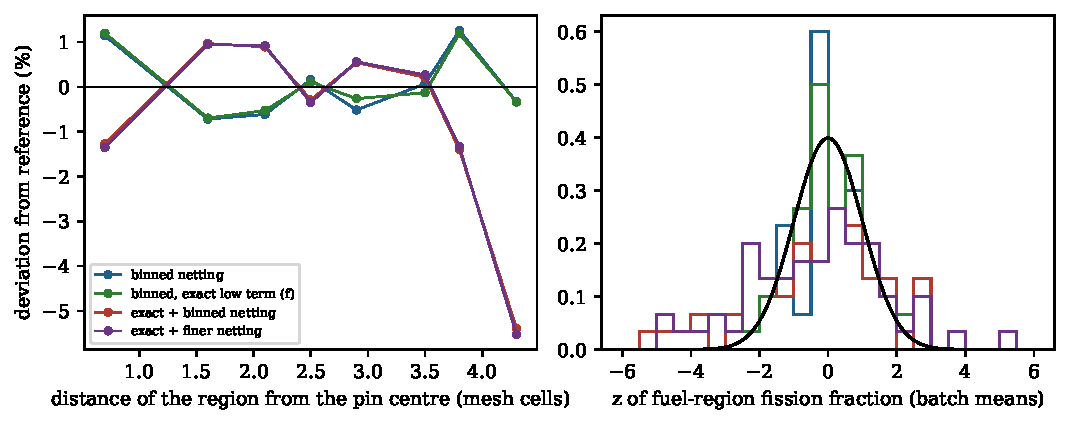
\includegraphics[width=\textwidth]{figures/stage8_shape.pdf}
\caption{Fission (or $\nu$-fission) rate by fuel region, normalized to unit sum. Left: mean relative
deviation from the reference against the region's distance from the pin centre. Right: histogram of
standardized differences (batch-means errors), against the standard normal density.}
\label{fig:s8:shape}
\end{figure}

\paragraph{The fission-rate shape.} With the CE correction tally (the first campaign), the fuel-region
shape agrees with the reference: $\chi^2=66$ for 60 regions, and no radial trend
(Figure~\ref{fig:s8:shape}). The $\pm1\%$ pattern that both binned variants share is the reference's
own noise, which both comparisons inherit.

The MG-controlled tally of the tuned campaign shows a $-5\%$ deficit in the outermost fuel regions,
and $\chi^2\approx255$. The pattern is the same for the coarse and fine netting, which share nothing
except the one-off MG low tally. That points to the low tally: its $4\times10^5$ backward points are
drawn once with a fixed seed and reused in every generation. Their sampling error is therefore
\emph{frozen}: it acts as a bias of the run rather than averaging away. It is largest in the small
partial regions cut by the pin surface, which receive the fewest uniform points.

This is a design error, not a property of the estimator. The low term of the MG control is the MG
reaction rate $V_R\sum_g\nu\Sigma_{f,g}\phi_{R,g}$, known in closed form from the field. It should be
computed that way, or at least redrawn every generation.

\subsection{Variance per particle and figure of merit}

\paragraph{Per particle.} The variance of $k$ per unit of work compares as follows:
\begin{itemize}
\item \textbf{RMC, tuned combined variant.} A generation processes $4\times10^3$ residual samples
  and $4\times10^4$ flights. The per-generation $k_n$ scatters by $0.021$, so the variance per
  particle-generation is $0.021^2\times4.4\times10^4\approx19$.
\item \textbf{Reference.} The batch-to-batch scatter of $k$ is $0.0041$ at $2\times10^4$ histories, so
  the variance per history is $0.34$.
\end{itemize}
Measured per particle and ignoring correlation, the method is $\approx60$ times worse. Counting the
correlation between generations, as the replica spread does (on both sides), it is $\approx1500$
times worse.

The per-particle variance is large because the residual estimate's absolute weight is large. In
the tuned run each generation's candidate bank holds about 12 units of absolute weight per unit of
fission production, before netting:
\begin{itemize}
\item $6.7$ from the scattering residual records;
\item $0.8$ from the fission residual after pooling ($3.1$ before);
\item $4.4$ from the children of the previous bank.
\end{itemize}
Netting keeps about $37\%$. The flights and netting only carry and contract what the residual
injects, so the residual estimator is the noise source. Its noise is not residual-scale: per sample
it is the integration noise of the high term over $\mathbf\Omega'$ and $E'$
(Section~\ref{sec:res:controlled}). Part of the scattering residual's signed mass is, in addition,
the amplitude term of Section~\ref{sec:iteration} (Section~\ref{sec:res:followup}).

\paragraph{Per second.} The figure of merit $1/(\sigma^2T)$ of $k$ for the tuned combined variant,
relative to the reference, is:
\begin{center}
\begin{tabular}{@{}lcc@{}}
\toprule
 & batch-means $\sigma$ & replica $\sigma$\\
\midrule
measured & $0.020$ & $0.0015$\\
projected (Section~\ref{sec:s8:projection}) & $0.068$ & $0.0049$\\
\bottomrule
\end{tabular}
\end{center}
The batch-means figure is optimistic and the replica figure, from only three replicas, is uncertain
by about a factor of two. The truth is nearer the replica figure.

The best measured $k$ figure of merit belongs to the low term in closed form (binned, exact low):
$0.043$ with batch means. It also has the smallest bias.

The shape figure of merit, the mean relative variance over the 60 fuel regions, is $10^{-3}$ of the
reference for every variant. The correction tally is dominated by its backward points and the bank's
collision estimator, and both carry the bank's full absolute weight into every region.

\subsection{Follow-up: the bias, the amplitudes, and history-based flights}\label{sec:res:followup}

The first measurement left three questions:
\begin{itemize}
\item whether the bias is the normalization bias of a noisy iteration or netting's deterministic bias;
\item where the noise comes from;
\item whether history-based flights, which make a generation fission-to-fission, shorten the
  correlation enough to pay for themselves.
\end{itemize}
Every run below is the tuned combined variant (40 inactive and 60 active generations, $N_\delta=2\times10^5$,
$N_B=4\times10^4$) unless stated otherwise. The runs are in
\code{results/stage8\_followup} under \code{examples/rmc}, and \code{stage8\_followup\_analysis.py}
analyses them.

\begin{table}[t]\centering\small
\caption{Follow-up runs. Columns: $n$, the number of replicas; $\Delta k$, the bias against the
reference with its standard error; paired, the difference from the baseline replica with the same
seed (same residual samples); $\overline{\Wabs}$, the bank's mean absolute weight; $\sigma_{gen}$, the
per-generation spread of $k_n$; $T$, the active time per replica in seconds; FOM$_k$, the figure of
merit relative to the reference. The errors of a replica mean use $\sigma_{gen}\sqrt{\tau/n_{gen}}$
with $\tau=21$ generations, measured from the nine independent baseline replicas; the first row uses
their spread directly.}
\label{tab:fu}
\setlength{\tabcolsep}{3.5pt}
\resizebox{\textwidth}{!}{%
\begin{tabular}{@{}lrrrrrrr@{}}
\toprule
run & $n$ & $\Delta k$ (pcm) & paired (pcm) & $\overline{\Wabs}$ & $\sigma_{gen}$ & $T$ & FOM$_k$\\
\midrule
\csname @@input\endcsname figures/followup_table.tex
\bottomrule
\end{tabular}}
\end{table}

\begin{figure}[t]\centering
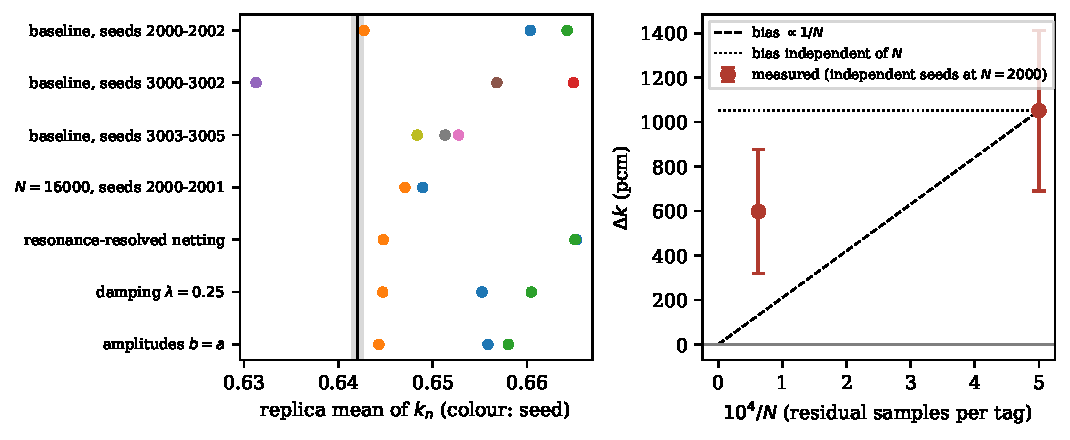
\includegraphics[width=\textwidth]{figures/followup_bias.pdf}
\caption{Left: replica means of $k_n$ for every run, coloured by seed. Replicas with the same seed
share their residual samples, which is why the seed-2001 replica (orange) is low in every run of the
first group. The vertical line and band are the reference and its replica spread. Right: the bias
against $1/N$, with the two simple models.}\label{fig:fu:bias}
\end{figure}

\paragraph{Independent seeds.} Six new replicas (seeds 3000--3005) give $k$ between $0.631$ and
$0.665$. With the original three, the nine independent baseline replicas give:
\begin{itemize}
\item $\Delta k=+1050\pm360$~pcm, a positive bias at $2.9\sigma$; eight of the nine replicas lie above
  the reference;
\item a replica spread of $0.0108$ against a per-generation spread of $0.018$ over 60 generations,
  which means an integrated autocorrelation time of $\tau=21$ collision generations.
\end{itemize}

\paragraph{The bias against $N$.} With $N=16000$ residual samples per tag (seeds 2000 and 2001):
\begin{itemize}
\item the per-generation spread falls from $0.021$ to $0.0066$, a factor of $3.2$, close to $\sqrt8$;
\item the bank's absolute weight falls from $4.4$ to $1.8$, because more samples per bin cancel
  better;
\item the bias is $+600\pm280$~pcm.
\end{itemize}
A bias proportional to $1/N$ would be $130$~pcm here; one independent of $N$ would stay at $1050$.
The measurement lies between the two and is $1.7\sigma$ from each (Figure~\ref{fig:fu:bias}). The
normalization bias is therefore at most part of the story, and the data cannot exclude a bias that
does not fall with $N$. Separating them needs two things: more replicas at large $N$, and a large-$N$
run whose netting is resolved finely enough that its own bias is negligible.

\paragraph{Resonance-resolved netting.} In this run, every fine bin of the lifts' grid in the three
groups from $0.625$~eV to $821$~keV is its own netting energy bin ($\approx90$ bins per decade). The
results:
\begin{itemize}
\item $\Wabs$ rises to $12.8$, because the bins are sparser and cancel less;
\item the paired difference from the baseline is $+260\pm120$~pcm.
\end{itemize}
So resolving the resonance range does not remove the bias; if anything it raises $k$ slightly. That
argues against netting's within-group smearing in that range as the cause. The test is incomplete
in two ways. The grid is about $0.025$ in lethargy, which does not resolve the narrowest resonances.
And the spatial and angular parts of the projection are unchanged.

\paragraph{Damped normalization.} Normalizing with $f_n^{0.25}$ instead of $f_n$ weakens the feedback of
a noisy $f_n$. The paired change is $-230\pm220$~pcm: consistent with a modest reduction, and with none.

\paragraph{Following amplitudes.} With $b=a$ (Section~\ref{sec:iteration}):
\begin{itemize}
\item $\Wabs$ falls from $4.4$ to $3.5$;
\item the paired change in $k$ is $-310\pm240$~pcm;
\item the figure of merit does not change, because $\sigma_{gen}$ does not.
\end{itemize}
The amplitude term is real, as the left of Figure~\ref{fig:fu:amp} shows. In the baseline, the
candidate's signed scattering mass varies with $a_s-b_s$ with a slope of $42.7$, the field's scattering
production per unit fission production. The correlation is $0.69$, so the amplitude term accounts for
about half of the variance of the scattering mass. Removing it lowers the absolute weight. But
$k_n$'s noise comes from the remaining residual noise, which is unchanged.

\begin{figure}[t]\centering
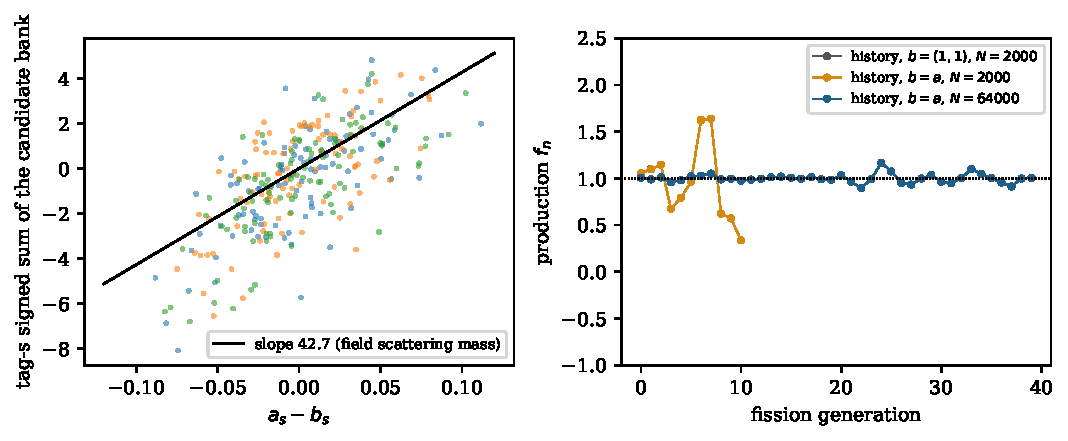
\includegraphics[width=\textwidth]{figures/followup_amplitude_history.pdf}
\caption{Left: signed tag-$s$ sum of the candidate bank against the field's amplitude offset $a_s-b_s$,
for every generation of the three baseline replicas. The slope is the field's scattering production
per unit fission production. Right: the production $f_n$ by fission generation with history-based
flights. With $b=(1,1)$ the run fails at the second generation; with $b=a$ and $N=2000$ it oscillates
and fails; with $b=a$ and $N=64000$ it is stable.}\label{fig:fu:amp}
\end{figure}

\paragraph{History-based flights.} Each flight now continues through its scatterings (37 collisions
per history on average). With $N_\delta=2\times10^4$ histories per generation, the flights cost about
1~s per generation.

\emph{Stability.} With $b=(1,1)$ the iteration fails within two or three generations at $N=2000$ and
at $N=16000$. Damping the normalization ($\lambda=0.1$, $N=4000$) does not save it: all three
replicas fail within eight generations.

The cause is the amplitude term. A fluctuation of $f_n$ puts $42\,(a_s-b_s)$ of scattering mass into
the next residual. A history carries that mass to fission within one generation, at about $0.9$
units of fission production per unit, so the term feeds back on $f$ with a gain of about $40\times0.9$
per unit change of $1/f$, far above one. In the collision iteration the same mass reaches fission over
about 40 generations, and netting and normalization act on it in between.

With $b=a$ the amplitude term is gone. What remains is the residual's own sampling noise, now
delivered to fission in a single generation:
\begin{itemize}
\item at $N=2000$, $f_n$ fluctuates by about $30\%$, and the replicas fail after 11, 22 and 60
  generations;
\item at $N=64000$ ($32\times$ the samples, about one collision generation's worth per collision of a
  history), the run is stable, with:
  \begin{itemize}
  \item $f_n$ varying by $5\%$;
  \item $\Wabs=0.77$;
  \item a lag-1 correlation of $0.50$ ($\tau\approx3$ fission generations);
  \item $k=0.6512$, $+900\pm1100$~pcm, which is not informative;
  \item $47$~s per generation, $95\%$ of it residual sampling.
  \end{itemize}
\end{itemize}

\emph{Figure of merit.} The figure of merit is $2\times10^{-4}$ of the reference, about 9 times
below the collision iteration's $1.8\times10^{-3}$. Per generation, $\sigma_{gen}^2\tau$ is $0.0035$
against $0.0068$. But a generation costs 16 times more, because the residual must be sampled about 30
times more heavily per generation to keep $f_n$ stable.

\emph{What this says about the correlation.} Measured in neutron lifetimes, the collision iteration's
correlation is not long. $\tau=21$ collision generations is about half of a 37-collision lifetime,
while the fission-to-fission iteration has $\tau\approx3$ lifetimes. The apparent long correlation of
Section~\ref{sec:convergence} is long only in units of collision generations, which are cheap. The
real figure-of-merit gap is the variance injected per unit of work, and history-based flights do not
reduce it. They only change when it reaches fission.

\subsection{Toward a speedup: the residual estimator's efficiency}\label{sec:res:speedup}

The follow-up showed that the residual estimator sets the variance. This subsection measures that
estimator's efficiency directly, searches its options, and makes the iteration cheaper. It then
remeasures the whole method. The scans are in \code{examples/rmc/results/speedup}, made by
\code{residual\_efficiency.py}; \code{speedup\_analysis.py} draws the figures.

\paragraph{A measure of efficiency for the eigenvalue.} A generation's residual records enter the bank
and reach fission over the following generations. To first order, their effect on $k$ is their total
fission yield
\begin{equation}
Y=\big\langle 1,\;F\,(I-\mathcal S)^{-1}\hat r\big\rangle=\sum_i w_i\,\eta(\mathbf r_i,E_i),
\end{equation}
with $\eta$ the fission weight that a neutron emitted at $(\mathbf r,E)$ produces in its own
history: an importance for $k$. Two steps build the estimate:
\begin{itemize}
\item $\eta$ is tabulated once, by field region and 60 energy bins, from history flights of
  $2\times10^5$ states;
\item one large sample ($5\times10^4$ to $10^6$ destinations per tag) gives
  $\mathrm{Var}(Y)$ for $N=2000$ records per tag from its per-destination contributions.
\end{itemize}
$\mathrm{Var}(Y)$ times the sampling time measures the eigenvalue noise injected per second. Its
ranking agrees with the full iteration wherever both were measured.

\paragraph{Where the noise is.} In the Stage 8 configuration:
\begin{itemize}
\item the scattering residual carries $97\%$ of $\mathrm{Var}(Y)$; the pooled fission residual
  carries $3\%$;
\item within the scattering residual, fuel destinations above 100~keV account for $44\%$, and fuel
  destinations in the resonance range (4~eV--10~keV) for $36\%$;
\item at $J=8$ directions, about $60\%$ of the variance is direction noise: repeating the same
  destinations with $J=32$ and $J=128$ leaves a floor of $\approx0.011$ (at $N=2000$);
\item at $J=128$ the scattering residual is $4.5\%$ of the field's scattering emission in absolute
  value: $4\%$ in the fuel and $1.2\%$ in the graphite (medians).
\end{itemize}
The largest single contributions come from destinations within $0.01$~cm of the pin surface at
resonance energies, along the one or two directions that look into the graphite. There the
moderator's unshielded flux meets the $^{238}$U scattering resonances.

\begin{figure}[t]\centering
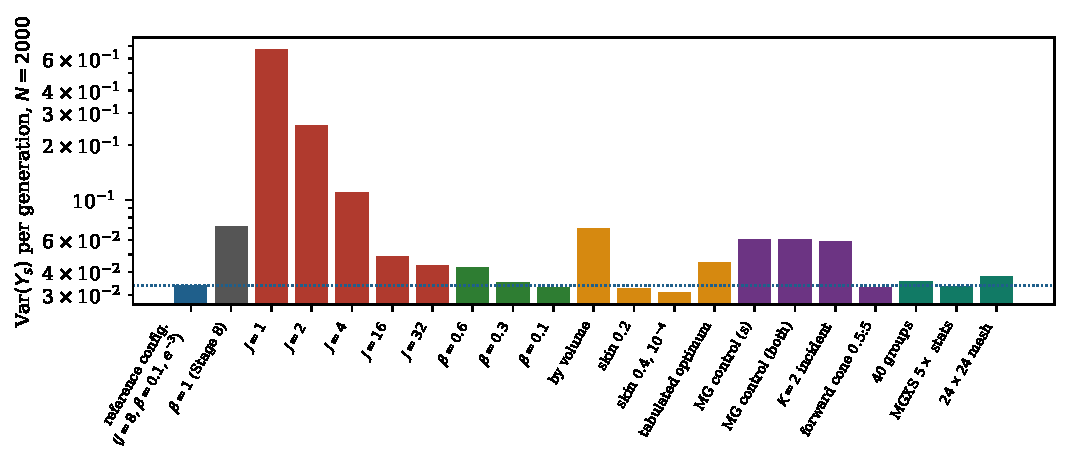
\includegraphics[width=\textwidth]{figures/speedup_scans.pdf}
\caption{Variance of the scattering residual's fission yield per generation ($N=2000$) for the options
tried. The direction, outgoing-energy ($\beta$), destination-by-volume and control scans vary the
Stage 8 settings ($\beta=1$, cutoff $e^{-4}$; variance $0.06$ at $5\times10^4$ samples, $0.07$ at
$10^6$). The skin, tabulated, cone and field scans vary the improved settings ($\beta=0.1$,
cutoff $e^{-3}$; dotted line).}\label{fig:sp:scans}
\end{figure}

\paragraph{What the options do} (Figure~\ref{fig:sp:scans}, Table~\ref{tab:sp:scans}):
\begin{itemize}
\item \textbf{Outgoing-energy proposal.} Drawing 90\% of the outgoing energies from the region's
  emission spectrum ($\beta=0.1$) instead of log-uniformly halves the variance. It also shortens the
  heavy tail: the ten largest of $5\times10^4$ samples carry $12\%$ of the second moment instead
  of $19\%$. This is the one large gain, and it has a second effect, described with the iteration
  below.
\item \textbf{Directions.} The variance falls with $J$ until the floor, and the cost rises with $J$.
  Per unit time, $J=4$ to $8$ is best.
\item \textbf{Destinations.}
  \begin{itemize}
  \item A skin proposal, which draws 20--40\% of the destinations at a log-uniform depth inside the
    pin surface, removes the extreme tail (top-ten share $6\%$) but only $10\%$ of the variance.
  \item A proposal tabulated from a pilot run (region $\times$ 100 energy bins,
    $\propto\sqrt{n_b\,m_{2,b}}$) is worse. Its bins are far wider than the resonances, so it
    misplaces the samples within them.
  \end{itemize}
\item \textbf{Controls.} The MG control on the same paths, more incident energies on the sampler
  route, and a forward cone of directions for forward-peaked fast kernels leave the variance
  unchanged or raise it. The MG control's production tracks the CE production closely overall
  (correlation $0.99$), but not where the variance is: at the CE fine structure in energy.
\item \textbf{The field.} 40 groups instead of 8, five times the MGXS statistics, or a $24\times24$
  source-region mesh leave the variance unchanged. Within these options, neither the group
  structure, the MGXS noise, nor the spatial resolution sets the residual's noise. Material-level
  lifts and isotropic flat emission are what the field cannot represent near the pin surface.
\end{itemize}

\begin{table}[t]\centering\small
\caption{Variance of the residual's fission yield per generation ($N=2000$ per tag) for each option:
scattering ($s$) and fission ($f$), and the share of the scattering second moment carried by the
ten largest samples.}\label{tab:sp:scans}
\begin{tabular}{@{}llrrr@{}}
\toprule
group & option & Var$(Y_s)$ & Var$(Y_f)$ & top ten\\
\midrule
\csname @@input\endcsname figures/speedup_scans.tex
\bottomrule
\end{tabular}
\end{table}

\paragraph{Engineering.} A residual sample's time is spent tracing backward paths: geometry, mesh
crossings, cross sections and attenuation. Four changes make the scattering residual $3.5$ times
faster (1.07~s to 0.31~s per 2000 samples), with identical results:
\begin{itemize}
\item a per-path cache of $\Sigma_t$ for each energy and material state, since a path alternates
  among few materials;
\item the field's energy bins found once per energy instead of once per segment;
\item dense region tables per meshed cell instance, instead of hash lookups;
\item an incremental regular-mesh traversal (Amanatides--Woo) in place of OpenMC's general
  \code{bins\_crossed}, and one transcendental function per segment and energy instead of two.
\end{itemize}
The per-generation correction tally is not needed for $k$. Its field part is the same every
generation up to the amplitudes, so it can be computed once. The $k$ runs below omit it.

\begin{table}[t]\centering\small
\caption{The iteration after the changes of this subsection, against the reference. The columns are:
the number of replicas; $\Delta k$ with its standard error, from 10-generation batch means pooled over
the replicas; $\overline{\Wabs}$; the per-generation spread of $k_n$; the active time per replica; and
the $k$ figure of merit relative to OpenMC (replica spread of the reference). Unless stated
otherwise, every run uses $N=2000$ per tag, $N_B=4\times10^4$, 40 inactive and 60 active
generations, and the combined cancellation.}\label{tab:sp:runs}
\setlength{\tabcolsep}{3.5pt}
\resizebox{\textwidth}{!}{%
\begin{tabular}{@{}lrrrrrr@{}}
\toprule
run & $n$ & $\Delta k$ (pcm) & $\overline{\Wabs}$ & $\sigma_{gen}$ & $T$ & FOM$_k$\\
\midrule
\csname @@input\endcsname figures/speedup_runs.tex
\bottomrule
\end{tabular}}
\end{table}

\paragraph{The iteration, remeasured} (Table~\ref{tab:sp:runs}). With $b=a$, $\beta=0.1$, a cutoff of
$e^{-3}$, $N_\delta=5\times10^4$ and the faster tracer:
\begin{itemize}
\item \textbf{Bias.} The eigenvalue bias at $N=2000$ falls from $+900$ to between $+120$ and
  $+600$~pcm, depending on the seeds. Nine independent replicas of these settings (one set of three with smaller banks) give
  $+350\pm125$~pcm.
\item \textbf{Correlation.} The integrated autocorrelation time falls from $\approx21$ generations to
  $\approx3$.
\item \textbf{Figure of merit.} It rises from $0.005$ to $0.08$--$0.12$ of OpenMC's (batch-means
  errors on both sides of the change), about $20$ times.
\end{itemize}

Ablations with paired seeds (3000--3002) tie the change in bias to the energy proposal: the baseline
gives $+900$~pcm, $b=a$ with the cutoff $e^{-3}$ gives $+1130$, and $b=a$ with $\beta=0.1$ gives $-75$. The log-uniform proposal's
heavy tail, a few samples carrying a large share of the second moment, did two things:
\begin{itemize}
\item it drove the long excursions of $k_n$ that made the error estimates so different;
\item through the iteration's nonlinear normalization, it produced most of the bias.
\end{itemize}

At $N=8000$ the per-generation spread halves, and the figure of merit is $0.08$--$0.17$, depending on
the replicas.

\paragraph{The remaining bias.} At $N=8000$ the error of $k$ is small enough to expose a systematic
offset. Six replicas give $+950\pm70$ and $+1070\pm100$~pcm (field placement).
Figure~\ref{fig:sp:bias} shows how it builds up: $k_n$ starts near the reference while the bank is
empty and rises over 20--30 generations, the time the scattering correction takes to reach fission.
Several observations constrain its cause:
\begin{itemize}
\item \textbf{Placement.} Re-sampling netted particles from the bin's own particles of the net's sign
  ('empirical' placement) lowers it to $+660\pm100$~pcm. Finer netting bins (12$\times$12 zones, 4
  sub-bins per group) lower it to $+690$ (one replica).
\item \textbf{Frequency.} Netting every second or fourth generation does not lower it in proportion
  ($+985$ and $+650$, one replica each).
\item \textbf{No netting.} Without netting the bank's absolute weight grows by the residual's injection
  every generation (about 7 units), and the run fails after 65 generations.
\item \textbf{The residual.} The scattering residual's mean fission yield from $10^6$ samples is
  $+0.006\pm0.009$ (density route), $-0.002\pm0.044$ (density-free) and $+0.016\pm0.012$
  ($\beta=1$). The routes agree, so no bias of the residual is visible at that precision.
\end{itemize}
So netting's projection explains part of the bias, but not all of it. Which other part of the
iteration contributes is the next question.

\begin{figure}[t]\centering
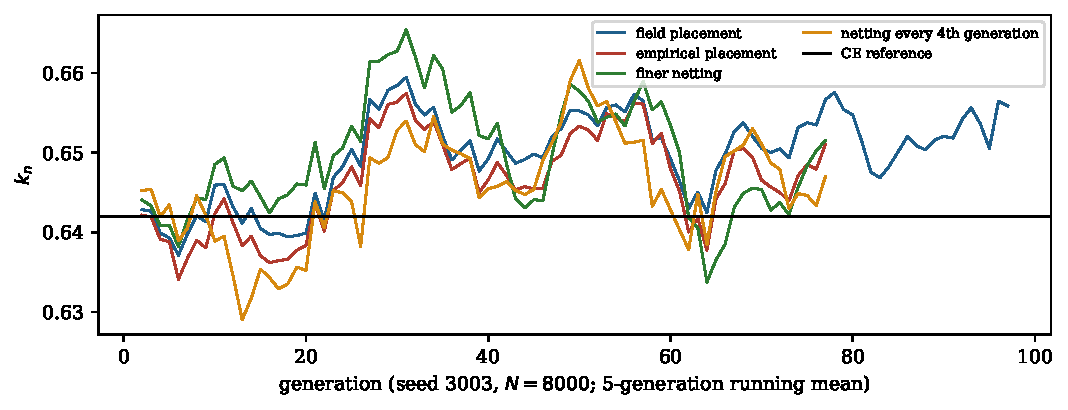
\includegraphics[width=\textwidth]{figures/speedup_bias_buildup.pdf}
\caption{$k_n$ by generation at $N=8000$ for four cancellation settings with the same seed (5-generation
running means). The runs share their residual samples, so their fluctuations coincide. $k_n$ starts
near the reference while the bank is empty, and rises over the 20--30 generations the scattering
correction needs to reach fission. Empirical placement and finer netting lower the plateau, but do not
remove it.}\label{fig:sp:bias}
\end{figure}

\paragraph{How far from a speedup.} The best configurations reach $0.1$--$0.17$ of analog Monte Carlo's
figure of merit for $k$, a factor of 6--10 short of break-even. The remaining levers:
\begin{itemize}
\item \textbf{Fixed costs.} Python-side cancellation (about 20\% of a generation) and bank handling
  could be moved to C++, a factor of about 1.3.
\item \textbf{Larger $N$.} Amortizing the fixed costs further gives at most 1.5.
\item \textbf{Fewer directions per unit of noise.} A per-stratum allocation of directions, more where
  direction noise dominates (fuel above 10~keV), gives an estimated 1.2--1.5.
\end{itemize}
These multiply to about 3. Closing the rest needs a residual that is smaller where it matters: lifts
resolved in space near the pin surface, or an anisotropic field emission. The measurements bound how
small it must be. A scattering residual that is a fraction $\varepsilon$ of the scattering emission
has an absolute fission yield of about $\varepsilon\,\bar n_c$ per unit of fission production, with
$\bar n_c\approx37$ the number of collisions in a neutron's life. With $\varepsilon\approx4.5\%$
here, that is about 1.7: larger than the production itself. The method beats analog Monte Carlo only
when $\varepsilon\,\bar n_c\ll1$. In graphite that means a field accurate to well below 1\% locally;
in light water, with $\bar n_c\approx20$, about twice that.

\subsection{Resonance-resolved lifts and several energies per trace}\label{sec:res:lifts}

The speedup study ended with two open items: a bias of $+650$ to $+1000$~pcm, and a scattering
residual too noisy by a factor of 6--10. This subsection finds the cause of the first, makes the
scattering residual about five times more efficient, and finds that a different term now limits
the method. The runs are in \code{examples/rmc/results/speedup2}.

\paragraph{What the direction noise is.} Anisotropic emission was to be the next field improvement.
Before implementing it in random ray, its potential was measured. The scattering residual was
evaluated at fixed destinations and energies for 12 outgoing directions (128 incident directions
each), and split into its angle average and the rest:
\begin{itemize}
\item the angular part carries $15\%$ of the residual's second moment overall;
\item in the fuel it carries $13\%$, and in the fast fuel about $1\%$.
\end{itemize}
An anisotropic field could remove at most that share, so it was not implemented.

The per-direction data show what the noise is instead. At a fixed destination and outgoing state,
the CE production of single incident directions scatters by $13$--$100\%$ about its mean. The MG
production on the same paths varies by about $5\%$ and is uncorrelated with it. Each direction has
its own image energy $E'=E/\gamma_A(\mu_0)$ for each nuclide, and the path's flux $\psi(E')$ has
resonance structure: a ray that crosses the pin at an energy on a $^{238}$U resonance arrives
attenuated, and a neighbouring energy does not. The direction noise is therefore noise in
\emph{energy}, sampled once per direction. No smooth control can follow it. Three were tried:
\begin{itemize}
\item a control with the region's isotropic flux at the same image energies: correlation $0.95$ in
  the fast fuel, where the structure is the kernel's and not the flux's, but only $-25\%$ in the
  total variance;
\item a control with the local uncollided flux $Q/\Sigma_t$: no gain;
\item incident directions drawn from a learned distribution of the scattering cosine: $-15\%$.
\end{itemize}

\paragraph{Several outgoing states per destination.} If the noise is in energy, more energies per
trace average it. Each destination now carries $K_{out}$ outgoing states (energy and direction), each
a density record of its own, and all of them share the destination's $J$ backward traces: the image
energies of every state ride on each path. Three details matter:
\begin{itemize}
\item \textbf{Stratified energies.} The $K_{out}$ energies are stratified over the proposal
  (systematic sampling with one random offset), so every destination covers the energy range. This
  matters in the fast fuel: there the sampler-route particles (inelastic scattering) of a
  destination are offset by the low term at fast outgoing energies, and only on average.
\item \textbf{Image roulette.} In the fuel each state has one image per nuclide, and trace nuclides
  contribute little. Nuclide $n$'s image is kept with probability
  $p_n=\min(1,\max(0.25,4\times\text{its share of }\Sigma_s))$ and weighted by $1/p_n$. A floor of
  $0.05$ is too low: a rare image on a resonance then carries a weight of 20.
\item \textbf{Tabulated incident energies} for the sampler route, proportional to its production
  times the lifted flux. A log-uniform draw over twelve decades mostly misses the inelastic
  thresholds.
\end{itemize}
The estimate stays unbiased for any $K_{out}$: every record carries $K_{out}$ times its draw density.

\begin{table}[t]\centering\small
\caption{The scattering residual with $K_{out}$ outgoing states per destination ($J=8$, $\beta=0.1$,
cutoff $e^{-3}$, $N=2000$ destinations): variance of the fission yield per generation and time per
generation. The last column is their product relative to $K_{out}=1$ with the first lifts.}
\label{tab:lifts:ko}
\begin{tabular}{@{}llrrr@{}}
\toprule
lifts & $K_{out}$ & Var$(Y_s)$ & time (s) & Var $\times$ time\\
\midrule
200 fine bins per group & 1 & 0.0338 & 0.32 & 1\\
 & 4 (independent energies) & 0.0103 & 0.68 & 0.65\\
 & 8 (stratified, roulette, tabulated incident) & 0.0059 & 0.93 & 0.51\\
 & 16 & 0.0028 & 1.43 & 0.37\\
resonance-resolved (4000 bins, 4~eV--5.5~keV) & 1 & 0.0290 & 0.31 & 0.83\\
 & 8 & 0.0043 & 0.96 & 0.38\\
 & 16 & 0.0023 & 1.49 & 0.32\\
\bottomrule
\end{tabular}
\end{table}

The variance falls nearly as $1/K_{out}$ (Table~\ref{tab:lifts:ko}), almost as if each state were an
independent destination, while a state costs about a sixth of a destination. With $K_{out}=16$ and the
lifts below, the scattering residual's variance at equal time is about a third of what it was. In the
iteration, the bank's absolute weight falls below one for the first time ($\Wabs\approx0.85$).

\paragraph{Resonance-resolved lifts remove the bias.} The lifts had 200 fine bins per group. In the
group from 4~eV to 5.5~keV that is a lethargy width of $0.036$ per bin, ten times wider than the
$^{238}$U resonances. The scattering emission of the fuel keeps resonance structure, because a
collision with $^{238}$U changes the lethargy by at most $0.017$. So the low term $U(E)$ averaged
over structure that the CE production $C(E)$ resolves, and the residual in the fuel carried large
positive and negative parts within every lift bin.

New lifts were tallied with 4000 bins in that group (lethargy width $0.0018$) and 800 in the next.
The field's group emission is unchanged; only the within-group shapes are finer. Two results:
\begin{itemize}
\item \textbf{Variance.} The scattering residual's variance falls by $15$--$30\%$
  (Table~\ref{tab:lifts:ko}).
\item \textbf{Bias.} With the same seeds and settings ($N=8000$, $K_{out}=1$, empirical placement),
  the bias goes from $+664\pm102$~pcm to $-31\pm80$~pcm (the error from batch means; the three
  replicas agree within $30$~pcm). With $K_{out}=16$, nine replicas give $-86\pm58$~pcm.
\end{itemize}
This settles the cause of the bias. It was netting: not through the netting bins of the resonance
range, which the follow-up tested, but through what was in them. The unresolved low term made the
correction carry large cancelling parts on the scale of single resonances, and every netting
smeared them within its bins. With lifts that resolve the resonances, the correction no longer has
that structure, and netting's projection error falls below the present precision of about 80~pcm.

\paragraph{What limits the method now.} With the scattering residual quieter, the figure of merit
should have risen. It did not: the best configuration ($K_{out}=16$, resonance-resolved lifts,
$N=2000$, $N_f=6000$) gives $\sigma(\bar k)=0.0013$--$0.0017$ over 60 generations in about 145~s. That
is a figure of merit of $0.09$--$0.16$ of OpenMC's, the same as before within its uncertainty.

The reason is a noise source that had been hidden. The per-generation spread of $k_n$ is now white
(no autocorrelation) and proportional to $1/\sqrt{N_f}$, the number of \emph{fission} residual
samples:
\begin{center}\small
\begin{tabular}{@{}lrr@{}}
\toprule
run & $N_f$ & $\sigma_{gen}$\\
\midrule
$N=2000$, $K_{out}=8$ & 2000 & 0.0168\\
$N=4000$, $K_{out}=8$ & 4000 & 0.0126\\
$N=2000$, $K_{out}=16$ & 6000 & 0.0095\\
$N=8000$, $K_{out}=1$ & 8000 & 0.0088\\
\bottomrule
\end{tabular}
\end{center}
This is the noise of one number: the CE fission production of the field's own first-flight flux,
\begin{equation}
X=\big\langle\nu\Sigma_f,\;\phi^{CE}[a\,\Qmg]\big\rangle,
\end{equation}
which enters every $k_n$ through the fission residual's mass. $X$ is a constant of the frozen field.
Estimating it directly and averaging the estimates over the generations
(\code{-{}-field-production}) removes the white noise: $\sigma_{gen}$ falls from $0.0095$ to
$0.003$. But the error of the running mean is then shared by every generation, and the spread of
replica means stays at $0.002$.

The eigenvalue cannot be known better than $X$: $\sigma_k/k\ge\sigma_X/X$. And $X$ is expensive to
estimate, because no variance reduction is in place for it:
\begin{itemize}
\item the MG control on the same paths lowers its variance only from $(1.7\%)^2$ to $(1.2\%)^2$ per
  $2\times10^4$ points;
\item for the fission residual, more incident energies or directions per sample lower the variance
  only in proportion to their cost (Var $\times$ time is constant from 8 to 256 path-energies per
  sample).
\end{itemize}
Reaching the reference's $0.077\%$ in $X$ with the present estimator takes about as long as the
reference itself. This term, not the scattering residual, now sets the figure of merit.

\paragraph{Where a speedup has to come from.} The method's premise holds for the shape of the
correction: it is carried by signed particles whose absolute weight is now below the fission
production. It does not yet hold for the one scalar $X$, which is estimated at analog-like cost. The
candidates:
\begin{itemize}
\item \textbf{A correlated control for $X$.} Evaluate the CE and the lifted-MG fission production
  at the same incident energies on the same path, $\nu\Sigma_f(E')\,[\psi^{CE}(E')-\psi^{MG}_{g}h_\phi(E')]$,
  so that only the flux difference is sampled. The flux-difference control of the sampler route did
  this for the high term of the fission residual (4.7 times, Section~\ref{sec:res:controlled}); it
  has to be combined with destination pooling.
\item \textbf{Importance in the thermal range.} Most of $X$ is thermal fission in the pin's outer
  layer. Destinations by the field's fission emission and incident energies by
  $\nu\Sigma_f\phi$ are not yet used for tag $f$.
\item \textbf{A field that carries $X$.} If the MG cross sections were condensed with the CE flux of
  the field's own emission, the MG and CE fission productions of the field would agree by
  construction, and $X-X^{MG}$ would be a second-order quantity.
\end{itemize}

\subsection{The field's fission production, the eigenvalue update, and exact cancellation}\label{sec:res:X}

Section~\ref{sec:res:lifts} left one scalar as the limit: $X$, the CE fission production of the
field's first-flight flux. This subsection removes that limit, finds the next one in the eigenvalue
update itself, and answers two questions about cancellation. The runs are in
\code{examples/rmc/results/speedup3}.

\paragraph{An importance-sampled estimator of $X$.} The estimators so far drew backward points
uniformly in space and incident energies from the lifted flux. The score
$\nu\Sigma_f(E')\,\psi(E')/p$ then varies by orders of magnitude, with the $1/v$ cross section and
the fission resonances. The new estimator (\code{field\_fission\_production}) draws from the field's
own lifted fission rate on the lifts' fine grid:
\begin{equation}
p(\mathbf r,E')\;\propto\;\phi_{R,g(E')}\,h_\phi(E')\;\nu\Sigma_f(E'_i),\qquad \mathbf r\in R,\ E'\in\text{fine bin }i,
\end{equation}
with an isotropic direction. The score is then the total of those weights times two ratios near
one: the CE $\nu\Sigma_f$ at $E'$ to its value at the bin's midpoint, and the path's CE angular
flux to the region's lifted scalar flux per unit solid angle. It is unbiased for any lifts, because
the density is evaluated exactly.

\begin{center}\small
\begin{tabular}{@{}lrr@{}}
\toprule
estimator of $X$ & relative error $\times\sqrt{\text{seconds}}$ & variance $\times$ time\\
\midrule
uniform points, energies from the lifted flux & 0.87\% & 1\\
the same with the MG control on the path & 0.61\% & 0.5\\
lifted fission rate, 4 energies per point & 0.071\% & 1/150\\
lifted fission rate, 16 energies per point & 0.057\% & 1/230\\
\bottomrule
\end{tabular}
\end{center}
With the resonance-resolved lifts, the reference's $0.077\%$ is reached in about one second. With
the 200-bin lifts the gain is only about 9 in variance: the fission resonances must be resolved by
the proposal. In the iteration, $X$ is estimated with 5000 points per generation and averaged over
the generations (0.13~s per generation).

\paragraph{The white noise is gone; a long memory remains.} With this estimate, the per-generation
spread of $k_n$ falls from $0.0095$ to $0.0024$. But the spread of the replica means is also
$0.0024$ (six replicas, 60 active generations each): within a replica, the deviation of $k_n$
persists for the whole active phase. The lag-1 autocorrelation is $0.6$--$0.7$.

The cause is the eigenvalue update, not an estimator. In the emission-source form
$k_{n+1}=k_nf_n$, and the fission emission is rebuilt with $1/k_{n+1}$. An error in $k_n$
therefore changes the fission-born source at once, but the production $f$ responds only when
those neutrons have slowed down and caused fission, about one neutron lifetime (37 collision
generations) later. The loop that corrects $k$ has a delay of a lifetime, so $k_n$ carries every
past fluctuation for tens of generations. A 60-generation active phase then holds only two or
three independent values of $k$. With $\sigma(\bar k)=0.0024$ in 118~s, the figure of merit
is about $0.06$--$0.4$ of OpenMC's, depending on the error estimate, and no better than before on
the replica estimate.

\paragraph{History-based flights, revisited.} A fission-to-fission generation closes that loop within
one generation, and its bank is small. With the present estimators the history-based iteration is
stable at $N=2000$ (it needed $N=64000$ in Section~\ref{sec:res:followup}), with
$\Wabs\approx1.1$. But $k_n$ now oscillates with a period of about six generations and an amplitude
of $\pm15\%$ (autocorrelation $+0.5$, $-0.4$, $-0.8$ at lags 1--3), and the replica means scatter by
$0.005$. Two normalization variants were tried:
\begin{itemize}
\item fixed amplitudes $b=(1,1)$: fails within four generations, as before;
\item damped normalization ($\lambda=0.3$): the per-generation spread falls from $0.10$ to $0.033$,
  but the oscillation and the replica spread ($0.006$) remain.
\end{itemize}
The oscillation comes from the same update. With following amplitudes, $a_{s}$ and $a_f$ are
integrators ($a_{s,n+1}=a_{s,n}/f_n$, $a_{f,n+1}=a_{f,n}/f_n^2$), and $k_n$ is a third. In history
mode their restoring forces act with a delay of one or two generations and a gain near one: an
underdamped loop. So the fission-to-fission bank is cleaner, as expected, but the per-tag
normalization of Section~\ref{sec:iteration} is the wrong controller for it.

\paragraph{What to change next.} The estimators are no longer the limit: the scattering residual,
$X$ and the bank are each well below the present error. The limit is the controller that turns
them into $k$. Section~\ref{sec:res:grouped} implements an eigenvalue estimate without that memory,
and the exact cancellation at fission births that this section had left open.

\subsection{Grouped cancellation at fission births, and a balance eigenvalue}\label{sec:res:grouped}

This subsection implements two things and measures each: the exact grouped cancellation at fission
births of the companion proposal, and an eigenvalue update without memory. The runs are in
\code{examples/rmc/results/speedup4}.

\paragraph{Grouped cancellation: the estimator.} A bank entry is either a directional particle or an
\emph{emission record} $w_j\,\delta_{\mathbf x_j}P_j$: a site with an emission law that has not been
sampled yet as far as the estimator is concerned. Two laws are implemented:
\begin{itemize}
\item a fission birth: isotropic, at its sampled energy $e_j$;
\item an elastic scattering off a stationary target (incident energy above $400\,kT$): the record
  keeps the incident energy $\varepsilon_j$, the incident direction $\Omega_j$ and the nuclide. In a
  direction $\mathbf d$, with $\mu=\Omega_j\!\cdot\!\mathbf d$, the outgoing energy is
  $e_j=\varepsilon_j\,\gamma_A(\mu)$ and the density per solid angle is
  $p_{\text{lab}}(\mu\,|\,\varepsilon_j)/2\pi$.
\end{itemize}
Every other entry is directional: fresh residual particles, inelastic and thermal scatterings.
Groups are fixed from the incoming bank before the flights (records sorted by zone, law and energy
decade, in runs of $G$). A flight that causes fission at
$y=(\mathbf x,\ \text{nuclide }\ell,\ E_f)$ after a path shorter than $d_{\max}$ gets the weight
\begin{align}
W_G(y)&=\frac{\sum_{j\in G}J_j(y)}{\sum_{j\in G}m_j\,q_j(y)},\qquad
J_j=\frac{w_j\,\nu_\ell(e_j)}{k}\,q_j ,\\
q_j(y)&=\sum_{\text{paths}}a_j(\mathbf d)\,\frac{e^{-\tau(e_j)}}{r^2}\,\sigma_{f,\ell}(e_j)\,\chi_\ell(E_f\,|\,e_j),
\end{align}
with $m_j=N_\delta|w_j|/\Wabs$ the expected number of flights of member $j$, and the sum over the
reflected paths shorter than $d_{\max}$. A group of one gives back the ordinary weight. The code is
\code{rmc::grouped\_fission\_weight} and \code{GroupedFissionCancellation}
(\code{examples/rmc/cancellation.py}).

\paragraph{It is exact.} Gate G8.10 flies 2000 signed parents once, turns the children into
records, flies them again, and compares the fission grandchildren's weight in four bins of emitted
energy with ordinary and with grouped weights, over 120 repetitions of both flights. The paired
differences are $0.1$, $-1.4$, $0.7$ and $0.6$ standard errors, and a standard error is $0.7$--$1.1\%$
of the eligible weight per bin. The eligible absolute weight falls from $59.9$ to $23.5$ with $G=8$.

\paragraph{It is not sufficient.} Table~\ref{tab:res:grouped} gives the tuned configuration of
Section~\ref{sec:res:X}, without and with netting.

\begin{table}[t]\centering\small
\caption{Grouped cancellation at fission births ($G=32$, $d_{\max}=3$~cm). Without netting: one
replica, generation 7. With netting: three replicas, 60 active generations, same seeds in both
rows.}\label{tab:res:grouped}
\begin{tabular}{@{}lrrrrr@{}}
\toprule
 & $\Wabs$ & fission births & eligible & eligible $\sum|w|$ & all fission $\sum|w|$\\
\midrule
no netting, regional kernel & $52.7$ & & & & \\
no netting, grouped & $50.5$ & 248 & 105 & $0.383\to0.095$ & $0.92\to0.63$\\
netting, regional kernel & $0.94$ & 438 & 41 & & \\
netting, grouped & $0.95$ & 438 & 32 & $0.0026\to0.0021$ & $0.0349\to0.0345$\\
\bottomrule
\end{tabular}
\end{table}

\begin{itemize}
\item \textbf{Without netting the bank grows as before}: by $6.4$ in absolute weight per generation,
  with or without grouping. Grouping removes three quarters of the eligible fission weight, but
  fission births carry $2\%$ of the bank's weight. The scattering children carry the rest, and the
  method does not act on them: two members reach a site with different incident states, and their
  scattering laws there lie on different kinematic surfaces.
\item \textbf{Only a minority of fission births are eligible}: $42\%$ without netting and $7\%$
  with it. In this lattice most fission is thermal, and its parent is a thermal scattering in
  graphite. That law is tabulated with discrete outgoing angles and has no density to evaluate.
  With netting, most of the remaining weight is fresh residual particles, which are directional.
\item \textbf{With netting it changes nothing measurable}: $k=0.63925$ against $0.63920$ on the
  same seeds, and a replica spread of $0.0025$ against $0.0026$.
\end{itemize}
So the answer to ``is it sufficient for weight cancellation'' is no, for a structural reason: the
weight that must cancel is scattering weight. The grouped estimator is kept as an exact, tested
component (it generalizes the regional kernel of Section~\ref{sec:cancellation}, which is the
special case of isotropic members); it would matter in a fast system, where fission births follow
elastic or fission-born parents.

\paragraph{A balance eigenvalue.} The update $k_{n+1}=k_nf_n$ measures the eigenvalue through the
growth of the fission production from one generation to the next. In a collision-by-collision
iteration that growth is $1+(k/k_n-1)/\Lambda$ with $\Lambda\approx37$ collisions per lifetime, so a
generation corrects $1/\Lambda$ of the error in $k_n$ and the noise of $\Lambda$ generations
accumulates in it. The balance of one generation's flux has no such factor:
\begin{equation}
k^{\text{bal}}_n=\frac{P_n}{L_n},\qquad
P_n=\langle\nu\Sigma_f\,\phi_n\rangle,\qquad
L_n=\langle\Sigma_a\,\phi_n\rangle-\langle\text{gain of multiplying scatterings}\rangle .
\end{equation}
For the eigenfunction of the iteration run with a wrong $k_n$ (growth $\lambda$ per generation, tag
masses $M_s$, $M_f$), $L=M_f+(1-\lambda)M_s$ and
$k^{\text{bal}}\approx k_n\,(1+(\lambda-1)(1+M_s/M_f))=k_n(1+\Lambda(\lambda-1))$: the full correction
in one generation, from tallies whose noise is not multiplied by $\Lambda$. The pieces are:
\begin{itemize}
\item the field's part of $L$, $a_sL_s+a_fL_f$: two constants of the frozen field like $X$,
  estimated by the same importance-sampled backward estimator with the net loss cross section
  (\code{field\_production(score='loss')}; $\Sigma_t$ minus the production of every non-fission
  channel) and averaged over the generations;
\item the bank's part of $L$ and of $P$: collision estimators over the flights
  ($w\,\Sigma_a/\Sigma_t$ and $w\,\nu\Sigma_f/\Sigma_t$ at every collision, less the analog gain of
  multiplying scatterings), in place of counting about 440 analog fission births;
\item the update: both tags are normalized by $P_n$ alone, and
  $k_{n+1}=\sum P/\sum L$ over the last 20 generations. The run's estimate is $\sum P/\sum L$ over
  the active generations.
\end{itemize}
On the four-region toy the balance update converges to the CE eigenvalue with less than half the
error of the production update in each of the first five generations (\code{test\_driver\_toy.py}).

\paragraph{Result.} Table~\ref{tab:res:balance} compares the updates in the tuned configuration
($K_{out}=16$, resonance-resolved lifts, $N_\delta=5\times10^4$, 40 inactive and 60 active
generations). The error of a replica is the spread of the replica estimates, the measure on which
Section~\ref{sec:res:X} found $0.05$.

\begin{table}[t]\centering\small
\caption{The eigenvalue with the production update and with the balance update. $\Delta k$ against
the analog reference ($\sigma=0.00049$ in 151~s). FOM is $1/(\text{spread}^2\,T)$ relative to the
reference, with the 68\% interval that the number of replicas allows.}\label{tab:res:balance}
\setlength{\tabcolsep}{4pt}\footnotesize
\begin{tabular}{@{}lrrrrrrl@{}}
\toprule
update, configuration & repl. & $\Delta k$ (pcm) & spread & per gen. & lag-1 & $T$ (s) & FOM\\
\midrule
production, $N=2000$ & 9 & $-86\pm58$ & 0.0024 & 0.0024 & 0.6--0.7 & 118 & 0.05\\
balance, $N=2000$ & 10 & $-42\pm32$ & 0.00102 & 0.0027 & 0.34 & 133 & 0.26 (0.14--0.38)\\
balance, $N=8000$ & 6 & $+17\pm38$ & 0.00092 & 0.0017 & 0.56 & 410 & 0.11 (0.04--0.17)\\
balance, $N=1000$, $10^4$ loss pts. & 18 & $-113\pm25$ & 0.00107 & 0.0040 & 0.27 & 100 & 0.32 (0.22--0.43)\\
the same, damping $\lambda=0.2$ & 12 & $-91\pm28$ & 0.00098 & 0.0042 & 0.28 & 93 & 0.41 (0.24--0.58)\\
balance, history flights & 2 of 3 & $+39\pm41$ & & 0.0051 & $-0.08$ & 395 & \\
\bottomrule
\end{tabular}
\end{table}

\begin{itemize}
\item \textbf{The memory of the update is gone.} The replica spread falls from $0.0024$ to $0.0010$
  at the same cost, and the lag-1 autocorrelation from $0.6$--$0.7$ to $0.3$. The figure of merit
  on the replica measure rises from $0.05$ to $0.26$ of OpenMC's, a factor of five.
\item \textbf{It is still below one.} The spread is three times what independent generations would
  give ($0.0027/\sqrt{60}=0.00035$). What remains is correlated over about eight generations and is
  not the residual's sample size: at $N=8000$ the per-generation spread falls to $0.0017$ but the
  replica spread does not move, and at $N=1000$ it does not rise.
\item \textbf{The field's net loss is now the least precise constant.} Its estimator reaches
  $0.27\%\cdot\sqrt{\text s}$, against $0.066\%\cdot\sqrt{\text s}$ for $X$: $69\%$ of the loss is
  resonance absorption in the fuel, where the path's angular flux differs from the lifted flux by a
  factor of order one (relative spread $1.0$ per point). With 5000 points per generation its
  running mean contributes about $0.0006$ to a replica's error, a third of the variance; with
  $10^4$ points, about $0.0004$.
\item \textbf{A bias appears at small $N$.} $-113\pm25$~pcm at $N=1000$, $-42\pm32$ at $N=2000$,
  $+17\pm38$ at $N=8000$: consistent with a term proportional to $1/N$. It does not come from
  dividing by the noisy production: damping the normalization to $P_n^{0.2}$ leaves it at
  $-91\pm28$ on the same seeds. Its origin is not identified; the candidates are the netting of a
  noisier candidate bank and the following amplitudes $b=a$, which multiply the residual's noise.
\item \textbf{History flights.} With the balance estimate, the per-generation spread of the
  eigenvalue is $0.005$ where $k_nf_n$ oscillated by $\pm15\%$, so the controller was indeed the
  cause of the oscillation. But the fission-to-fission bank is not netted: in one of three replicas
  it grew from $\Wabs=9$ to $106$ in eight generations and the production turned negative. At
  $5.5$~s per generation it is also three times as expensive.
\end{itemize}

\paragraph{Where this leaves the method.} The best unbiased configuration is the balance update at
$N=2000$: $\Delta k=-42\pm32$~pcm and a figure of merit of $0.26$ ($0.14$--$0.38$) of analog Monte
Carlo, from $0.05$. No speedup is demonstrated. The remaining factor of four has two identified
parts:
\begin{itemize}
\item the net loss of the field's flux, which needs an estimator for resonance absorption as good as
  the one for fission (a proposal that follows the self-shielded angular flux, or lifts by zone);
\item the correlated part of the bank's production and loss, which neither $N$ nor the
  normalization changes. The bank's flights ($N_\delta$), its compression ($N_B$) and the netting
  are the untested suspects.
\end{itemize}

\subsection{The field's constants, and where the figure of merit stands}\label{sec:res:constants}

Section~\ref{sec:res:grouped} named two limits, and this subsection measures both. The run data are
in \code{examples/rmc/results/speedup5}.

\paragraph{How much of the error is the constants.} A balance run estimates the field's production
$X$ and net loss $L$ as running means. The final running mean of each replica can be recovered
from its rows, and the replica estimates recomputed with the mean over all replicas in its place:
\begin{center}\small
\begin{tabular}{@{}lrrrr@{}}
\toprule
 & replicas & spread as run & with pooled $X$, $L$ & spread of $\hat L_s$ (relative)\\
\midrule
$N=1000$ & 18 & 0.00107 & 0.00080 & 0.063\%\\
$N=2000$ & 10 & 0.00102 & 0.00062 & 0.073\%\\
$N=8000$ & 6 & 0.00092 & 0.00020 & 0.091\%\\
\bottomrule
\end{tabular}
\end{center}
The net loss of the field is most of a replica's error at $N=8000$ and a large part at
$N=2000$. Its relative error is $-\delta L/L$ in $k$, because the field carries $99\%$ of the
absorption.

\paragraph{The loss estimator cannot be improved by a better energy proposal.} The estimator's error
is $0.28\%\cdot\sqrt{\text s}$, and its variance per point is $0.06+0.85/n_E$ with $n_E$ energies
per path: the energies are already at their optimum. The loss is $69\%$ in the group from 4~eV to
5.5~keV and $24\%$ in the next one. At a resonance peak the path's flux over the lifted flux is
$0.3$ for a path from inside the fuel and $12$ for a path that enters through the rim. Two proposals
that follow this structure were implemented (\code{field\_production(hyperfine=...)}):
\begin{itemize}
\item energies from bins of lethargy width $10^{-4}$ (or $3\times10^{-5}$) weighted with the
  narrow-resonance flux $\Sigma/(\Sigma_t+\sigma_e)$;
\item the same bins sorted into 16 classes of $\Sigma_t$, with the class chosen by the flux that a
  path with $d$ cm of fuel behind it would see,
  $W_c\,[(1-e^{-S_cd})/S_c+e^{-S_cd}/\sigma_e]$.
\end{itemize}
Neither changes the error ($0.28$--$0.30\%\cdot\sqrt{\text s}$), and the roulette cutoff does not
either ($e^{-3}$, $e^{-5}$, $e^{-8}$). The proposal's tables are now built once per field instead of
at every call. So the constants are computed before the run (\code{field\_constants.py},
\code{stage8.py --field-constants}): $L_s=1.5293$ and $X_s=0.9336$ to $0.01\%$, in about 1100~s for
$L$ and 150~s for $X$; two independent sets with hashed seeds agree ($1.5292\pm0.0003$,
$1.5297\pm0.0003$).

\paragraph{With the constants fixed.} Table~\ref{tab:res:constants} gives the balance iteration at
$N=8000$ with $J=4$, 8 and 16 directions per destination. With six replicas the spread is uncertain, so the
error of a replica is also estimated from batch means of 20 generations pooled over the replicas.

\begin{table}[t]\centering\small
\caption{The balance iteration with precomputed constants, $N=8000$, $N_f=2000$, six replicas.
FOM relative to the analog reference; the time of the constants is not included.}\label{tab:res:constants}
\setlength{\tabcolsep}{4pt}\footnotesize
\begin{tabular}{@{}lrrrrrrr@{}}
\toprule
 & $\Delta k$ (pcm) & spread & FOM & batch means & FOM & lag-1 & $T$ (s)\\
\midrule
$J=4$ & $-42\pm33$ & 0.00081 & 0.27 (0.11--0.43) & 0.00111 & 0.14 & 0.70 & 206\\
$J=8$ & $-46\pm13$ & 0.00033 & 0.93 (0.39--1.48) & 0.00060 & 0.28 & 0.56 & 366\\
$J=16$ & $-38\pm19$ & 0.00046 & 0.25 (0.10--0.40) & 0.00051 & 0.21 & 0.47 & 698\\
\bottomrule
\end{tabular}
\end{table}

\begin{itemize}
\item \textbf{About 0.3 of analog; no speedup.} With $J=8$ the figure of merit is $0.93$
  ($0.39$--$1.48$) on the replica spread but $0.28$ on batch means. The row for $J=16$ decides
  between them: twice the directions cannot have a larger error, and both of its estimates are
  $0.0005$. So the spread of $0.00033$ at $J=8$ is a low draw, the error there is near $0.0006$, and
  the figure of merit is about $0.3$, with $J=8$ the best of the three. The time of the constants
  is not counted: with the present loss estimator, the best split of time between the constants and
  the run lowers the figure of merit by a further factor of $0.6$.
\item \textbf{Residual sampling is the whole cost.} It takes $5.85$ of the $6.1$~s of a generation;
  flights take $0.15$~s and cancellation $0.07$~s. A stack profile gives $73\%$ of it to the
  backward flux: $25\%$ tracing, $30\%$ the loop over segments and energies, $10\%$ cross sections.
\item \textbf{The sampler's knobs are flat in the single-generation measure and not in the
  iteration.} The variance of the residual's fission yield times its time is $3.3$--$4.1\times10^{-3}$ for
  roulette cutoffs $e^{-3}$, $e^{-2}$, $e^{-1.5}$ and for $J=8$ or $4$. But in the iteration
  $J=4$ triples the variance for $1.8$ times less time, and $J=16$ lowers it by a third for $1.9$ times more. The single-generation measure also predicts
  an error of $0.002$ at $N=8000$, four times what the iteration has: netting removes most of the
  sampled noise before it reaches fission, so that measure no longer ranks configurations.
\item \textbf{A bias of about $-40$~pcm remains} at $N=8000$: $-42\pm11$ over the three rows, with
  $\pm25$ from the reference's four replicas. With the precise constants the earlier rows of
  Table~\ref{tab:res:balance} move down: their running means of $L_s$ were $0.04$--$0.1\%$ below
  the precise value, which raised $k$ by $26$--$64$~pcm.
\end{itemize}

\paragraph{Where this leaves the method.} On the graphite pincell the method is at about $0.3$ of
analog Monte Carlo for $k$ once the field's constants are known, and no tested change of the
sampler's parameters moves it. Three things would:
\begin{itemize}
\item a faster backward flux: the paths cross about a hundred mesh cells of graphite each, and a
  coarser source mesh in the moderator, or a tracer that integrates a flat source over a whole
  cell, would cut most of the tracing and of the segment loop;
\item an estimator of the field's net loss that follows the rim paths in the resonances, so that
  the constants cost seconds;
\item a single-generation measure that includes netting, so that the sampler can be tuned without a
  forty-minute run per configuration.
\end{itemize}

\subsection{Coarser mesh, forward rays for the loss, and a resonance-resolving low order}\label{sec:res:forward}

Three questions from Section~\ref{sec:res:constants} are answered here. The data are in
\code{examples/rmc/results/speedup6}.

\paragraph{A coarser source mesh does not help.} The field was solved again on a $4\times4$ mesh
(and $6\times6$) instead of $12\times12$, with the same lifts and its own constants. With
$N=8000$, $J=8$ and six replicas:
\begin{center}\small
\begin{tabular}{@{}lrrrrrr@{}}
\toprule
mesh & $\Delta k$ (pcm) & spread & batch means & lag-1 & $T$ (s) & FOM (spread; batch means)\\
\midrule
$12\times12$ & $-46\pm13$ & 0.00033 & 0.00060 & 0.56 & 366 & 0.93; 0.28\\
$4\times4$ & $-11\pm16$ & 0.00040 & 0.00069 & 0.76 & 267 & 0.88; 0.29\\
\bottomrule
\end{tabular}
\end{center}
A generation is $27\%$ faster, not the factor of two hoped for: mesh crossings are a minor part of
the backward flux. The error per generation is the same and its correlation is longer, so the
figure of merit does not move. The field's spatial resolution is not what limits the method, in
cost or in noise.

\paragraph{Forward rays for the field's net loss.} The backward estimator scores
$\Sigma\,\psi$ at a point, and at a resonance peak that product differs by a factor of forty between
a point at the rim and one inside the fuel. The new estimator
(\code{field\_first\_flight\_rates}) removes the point: a source neutron is drawn from the field's
emission and its ray is integrated analytically,
\begin{equation}
A_x(\mathbf r,\Omega,E)=\sum_{\text{segments}}\frac{\Sigma_x}{\Sigma_t}\left(e^{-\tau_{\text{in}}}-e^{-\tau_{\text{out}}}\right),
\end{equation}
so where on the ray the collision falls carries no noise, and the ray needs only the material of
each segment. Energies are drawn from the emission times a rational approximation of the loss
probability, $\Sigma_{\text{loss}}/(\Sigma_t+\sigma_e)$ in the fuel, on sub-bins of lethargy width
$10^{-4}$; regions are reweighted once by a pilot.
\begin{center}\small
\begin{tabular}{@{}lrr@{}}
\toprule
estimator of $L_s$ & relative error $\times\sqrt{\text{seconds}}$ & variance $\times$ time\\
\midrule
backward points, 4 energies per path & 0.28\% & 1\\
forward rays, 8 energies per ray & 0.17\% & 1/2.7\\
forward rays, 2 energies per ray & 0.12\% & 1/5.4\\
forward rays, 1 energy per ray & 0.08--0.11\% & 1/7 to 1/12\\
\bottomrule
\end{tabular}
\end{center}
The remaining variance is between rays, not between energies (0.4 relative per ray for any number
of energies): a ray along a corridor between pins never meets fuel. For the production $X$ the
backward estimator stays better ($0.066\%$ against $0.29\%$). Gate G8.12 checks the forward rates
against the backward ones.

With $4\times10^4$ rays per generation ($0.17$~s of $6.1$) and no precomputed constants, four
replicas give a spread of $0.00046$ and a batch-means error of $0.00059$, with
$\Delta k=-50$~pcm: the same as with constants computed beforehand. (Two more replicas were lost to
a restart of the machine.) The figure of merit of about $0.3$ therefore now includes everything.

\paragraph{Would a resonance-resolving low order help?} RESOLVE (Mylotte and Forget) transports the
coefficients of a data-derived energy basis and decodes a continuous, self-shielded spectrum per
region. It could enter this method in two ways, and each has a test with the present code.
\begin{itemize}
\item \textbf{As a better field.} Its emission would be closer to a fixed point of the CE operator.
  But the variance of the residual's fission yield does not respond to the field's quality:
  \begin{center}\small
  \begin{tabular}{@{}lr@{}}
  \toprule
  field & Var$(Y_s)$, $N=2000$\\
  \midrule
  8 groups, one within-group shape per material & 0.031\\
  8 groups, shapes by ring (4 in the fuel, 2 in the graphite) & 0.032\\
  361 groups (SHEM) & 0.029\\
  \bottomrule
  \end{tabular}
  \end{center}
  The sampled residual at a destination is the difference between a few samples of
  $K_s\psi^{CE}$ over direction and incident energy and the field's emission there. Its noise is
  the noise of those few samples, and it stays when the mean it estimates gets smaller.
\item \textbf{As a control on the backward path.} A low-order angular flux with resonance structure
  on the same path, whose integral over directions is the field's own emission, would cancel that
  noise sample by sample. The multigroup control on backward paths (Section~\ref{sec:impl:components}) is this
  construction, and with the 361-group field it leaves the variance at $0.030$ (from $0.029$) while
  the sampling takes 70 times longer. A lane basis would be cheaper per unit of resolution, but
  the control costs one exponential per lane and segment on every path, about fifteen times the
  present cost for 245 lanes, so it would have to lower the variance by more than that.
\end{itemize}
Neither test is RESOLVE itself: SHEM-361 resolves the resonances below about 23~eV only, and nearly
half of the noise was above 100~keV in the fuel. But both point the same way. On this problem the
method's error is the Monte Carlo integration error of the scattering production at each
destination, and a better low order does not reduce it. RESOLVE is not recommended as the next
step for this method.

\paragraph{Where this leaves the method.} About $0.3$ of analog Monte Carlo, everything counted,
with a bias of $-10$ to $-50$~pcm. The estimators, the controller, the constants and the field
have each been improved or exonerated; what remains is the number of collisions per neutron
lifetime (37 here), each of which needs its scattering production sampled. A problem with fewer
collisions per lifetime (a water lattice, a fast system) is the test that would tell whether the
method has a regime of its own.

\subsection{A correlated forward residual in the netting bins}\label{sec:res:correlated}

Every change of Sections~\ref{sec:res:speedup}--\ref{sec:res:forward} left the figure of merit for
$k$ near $0.3$ of analog Monte Carlo on this problem. This subsection identifies the structural reason
and describes a different estimator of the residual that removes it. It reaches several times the
analog figure of merit, but in the form tested here it is biased at the scale of the netting bins.
Section~\ref{sec:res:bcv} gives the unbiased form. The data are in
\code{examples/rmc/results/speedup7}.

\paragraph{Why the backward residual could not gain.} At a destination $(\mathbf x,E,\Omega)$ the
residual of tag $s$ is estimated as
\begin{equation}
\hat r(\mathbf x,E,\Omega)=\hat C(\mathbf x,E,\Omega)-U(\mathbf x,E),\qquad
\hat C=\frac1J\sum_{j=1}^{J}\frac{\nu\Sigma_s(E'_j\to E,\mu_j)\,\psi^{CE}(\mathbf x,E'_j,\Omega'_j)}{p(E'_j,\Omega'_j)},
\end{equation}
a few samples of the CE scattering production over incident direction and energy, minus the field's
exact emission $U$. The mean of $\hat r$ is small ($4.5\%$ of the emission), but its variance is the
variance of $\hat C$ alone, because $U$ is a constant: $\operatorname{Var}\hat r=\operatorname{Var}\hat C$.
The method therefore pays for a full Monte Carlo estimate of the scattering production at every
destination and gains nothing from the field's quality. This explains the null results of
Section~\ref{sec:res:forward}: a better field shrinks the mean of $\hat r$ and leaves its variance,
and a multigroup control on the backward path, whose kinematics differ from the CE sample's, is
barely correlated with it.

\paragraph{Forward rays from the field.} The estimator here starts from the other end. A source
neutron is drawn from the field's emission: a point $\mathbf x$ with density $\rho(\mathbf x)$
proportional to the region's volume times its emission, $n_E$ stratified energies $E_k$ from the
region's emission spectrum on the lifts' fine grid, and an isotropic direction $\Omega$. Its ray
is traced to the end of the roulette and integrated analytically. On a segment of length $\ell$ in
material $m$, entered with transmission $T_{\text{in}}$, the expected collided weight is
$T_{\text{in}}(1-e^{-\Sigma_t\ell})$, so where on the ray the first collision falls carries no
noise. The collided weight is summed per netting zone $z$:
\begin{equation}
c^{CE}_{k,z}=\sum_{\text{segments in }z}T^{CE}_{\text{in}}\left(1-e^{-\Sigma^{CE}_t(E_k)\ell}\right).
\end{equation}
The emission of the first collision is then deposited into the netting bins
$b=(\text{tag},z,e,d)$ (tag, zone, energy bin, direction bin). For a scattering, the outgoing energy
bin and direction bin come from $n_{\text{out}}$ forced collisions by OpenMC's own \code{scatter()}
off a nuclide drawn by its scattering cross section, per material and source energy; the deposit is
the collided weight times $\nu\Sigma_s/\Sigma_t$ (the production of every non-fission channel above
1~MeV) times the outgoing fractions. For a fission, the outgoing energy bin comes from forced
fissions (\code{sample\_fission\_neutron}) off a nuclide drawn by $\nu\sigma_f$, and the deposit is
the collided weight times $\nu\Sigma_f/\Sigma_t$. Every sum is an expected value over the collision
site and over the outgoing state, except for the $n_{\text{out}}$ forced collisions.

\paragraph{The multigroup partner on the same ray.} On the same ray, at the same source energies and
with the same roulette, a second deposit is scored with the multigroup cross sections of the group
$g_k$ of $E_k$: the collided weight $c^{MG}_{k,z}$ with $\Sigma^{MG}_{t,g_k}$, and the outgoing
emission $\nu\Sigma^{MG}_{s}(g_k\to g')$ and $\chi_{g'}\nu\Sigma^{MG}_{f,g_k}$, spread over the
energy bins of $g'$ with the lift's mass fractions and isotropically over the direction bins. The
per-ray difference
\begin{equation}
\Delta_b=\sum_k w_k\left(A^{CE}_{k,b}-A^{MG}_{k,b}\right),\qquad w_k=\frac{q(\mathbf x,E_k)}{\rho(\mathbf x)\,p(E_k)\,n_E},
\end{equation}
with $q$ the field's emission density per unit volume and energy and $A_{k,b}$ the deposit per unit
source weight, has as its expectation the CE first-collision emission of the field minus the
multigroup one, bin by bin. The multigroup deposit's own expectation is, by bin, the field's emission $F_b$ (tag $s$) and
$k_{MG}F_b$ (tag $f$, as productions): the field is the flat-source fixed point of exactly this
multigroup operator, the zones are unions of field regions, and both are isotropic. So
\begin{equation}
r_b=\mathbb E[\Delta_b]\quad\text{(tag $s$, unit amplitudes)},
\end{equation}
which needs neither $U$ nor a density at a destination. The identities hold only as far as the
field is converged; this is the first approximation of the form tested here.

\paragraph{Where the correlation is.} The two deposits share the ray, the source energy and the
roulette, so they are correlated wherever the CE and multigroup transmissions and emissions are
close. They are not close for the reactions that set $k$ directly. For the field's nu-fission
production and net loss, the difference is as noisy as the CE score alone (absolute error times
$\sqrt{\text s}$):
\begin{center}\small
\begin{tabular}{@{}lrrrr@{}}
\toprule
energies per ray & loss, CE & loss, CE $-$ MG & production, CE & production, CE $-$ MG\\
\midrule
1 & 0.0019 & 0.0060 & 0.0042 & 0.0039\\
8 & 0.0028 & 0.0039 & 0.0032 & 0.0027\\
32 & 0.0046 & 0.0027 & 0.0031 & 0.0029\\
\bottomrule
\end{tabular}
\end{center}
CE absorption sits in the resonance peaks, and the multigroup score spreads the same total evenly
over the group: the two agree only after an integral over energy. For the emission of the first
collision, weighted with an importance by material and group (the fission yield of a neutron born
there, from history flights), it is the opposite:
\begin{center}\small
\begin{tabular}{@{}lrrr@{}}
\toprule
energies per ray & per-ray spread, CE & per-ray spread, CE $-$ MG & error $\times\sqrt{\text s}$, CE $-$ MG\\
\midrule
1 & 11.5 & 3.5 & 0.0100\\
8 & 9.3 & 1.25 & 0.0066\\
32 & 9.0 & 0.63 & 0.0061\\
\bottomrule
\end{tabular}
\end{center}
(the total is 22.8). Thirty-six of the 37 collisions of a neutron's life are scatterings, mostly off
resonance in graphite, where the two transmissions nearly coincide, and the stratified source
energies average out the within-group kinematics. The backward sampler has
$0.058\cdot\sqrt{\text s}$ on the same scale: the difference is about 80 times cheaper per unit of
variance.

\paragraph{The residual is a constant of the frozen field.} In the bin basis, the residual per unit
amplitude of each source tag is a fixed vector, like the constants $X$ and $L$ of
Section~\ref{sec:res:grouped}. It is accumulated over the generations as running means $\bar D_s$,
$\bar D_f$ (per source tag), so its noise falls with the whole run instead of entering every
generation afresh. With the amplitudes $(a,b)$ and the eigenvalue $k$ of the generation, and the
multigroup identities, the residual of the field by bin is
\begin{align}
\text{tag }s:&\quad a_s\bar D_s+a_f\bar D_f+(a_s-b_s)F_s+(a_f-a_s)M_f,\nonumber\\
\text{tag }f:&\quad \left[a_s\bar D_s+a_f\bar D_f+(a_f-a_s)M_f\right]/k+(a_sk_{MG}/k-b_f)F_f,
\end{align}
with $M_f$ the multigroup deposit of the tag-$f$ source (zero in this form; with following amplitudes
$a_f-a_s$ is small). Its absolute size is $1.2$ against an emission of $87$; the backward residual
records carried $\Wabs=5.5$. $8\times10^5$ rays give it to $0.014$ (L2 over the bins).

\paragraph{Netting.} No residual particles are sampled. The bin totals of the bank's children and the
bin residual are summed and re-sampled by the binned netting with the field's shape
(\code{BinnedNetting(extra=\dots)}, placement \code{'field'}).

\paragraph{Implementation and tests.} \code{rmc::forward\_residual\_bins}
(\code{openmc\_rmc\_forward\_residual\_bins}) returns the running quantities per call: the
CE-minus-multigroup deposits and the multigroup deposits per source tag. A CE ray of 8 energies,
with the forced collisions, costs $73~\mu$s. Variant \code{forward} of \code{stage8.py} (options
\code{--forward-rays}, \code{--forward-energies}) accumulates them. Gate G8.13 checks that the
multigroup scores of the rays reproduce the field's balance (net loss $\langle1,Q^{MG}_f\rangle$,
production $k_{MG}\langle1,Q^{MG}_f\rangle$), and G8.14 that the multigroup deposits reproduce its
bins.

\paragraph{Result.} Six replicas of 40 inactive and 60 active generations, $4\times10^4$ rays of 8
energies per generation, the net loss from forward rays, the production from 5000 backward points,
the balance eigenvalue; against the reference of 14 analog replicas of Section~\ref{sec:res:bcv}:
\begin{center}\footnotesize\setlength{\tabcolsep}{4pt}
\begin{tabular}{@{}lrrrrrr@{}}
\toprule
residual & $\Delta k$ (pcm) & spread & per gen. & $\Wabs$ & $T$ (s) & FOM (spread; batch)\\
\midrule
backward samples, $N=8000$ & $-39\pm13$ & 0.00033--0.0006 & 0.00165 & 0.74 & 366 & 1.4; 0.41\\
forward bins & $-19\pm8$ & 0.00020 & 0.00028 & 1.27 & 253 & 5.5 (2.3--8.8); 21\\
\bottomrule
\end{tabular}
\end{center}
The figure of merit for $k$ is above analog Monte Carlo's: $5.5$ on the spread of the replica
estimates. The per-generation spread fell six times. The spread between replicas ($0.00020$) is twice
the batch-means error ($0.00010$), so it is set by what each replica accumulates once: $X$, $L$ and
the residual bins.

\paragraph{Why this form is not acceptable.} The method is meant to correct a biased deterministic
solution to reference quality. This form keeps three approximations that do not vanish with more
samples:
\begin{itemize}
\item the residual exists only as bin totals, placed with the field's shape: whatever the CE
  first-collision emission does within a bin (resonance structure within a group, spatial structure
  within a zone, anisotropy within a direction bin) is replaced by the field's;
\item the multigroup identities $M_s+M_f=F_s$ and $=k_{MG}F_f$ assume the field is the exact
  flat-source fixed point. Measured with $4\times10^5$ multigroup-only rays, the deposits differ from
  the field's bins by $0.154$ in L1 (noise $0.009$), and their tag-$f$ total is $0.999$ instead of
  $1$: the random-ray solution's own error, which the method must correct and this form does not;
\item the tag-$f$ deposit used the multigroup fission spectrum for the CE part too.
\end{itemize}
Most importantly, the residual has no particle representation, so replacing the netting by an
exact cancellation later would leave nothing to cancel: this form has no unbiased limit. Its bias
($-19\pm8$~pcm against a reference known to $\pm17$) is not larger than that of the netting in the
earlier variants, but it is of a different kind. Section~\ref{sec:res:bcv} also shows that part of
its gain came from these approximations.

\subsection{An unbiased form: the binned control variate}\label{sec:res:bcv}

\paragraph{The estimator.} Let $P$ be any unbiased particle estimate of the residual as a measure; here
the backward residual records of the earlier variants, with their exact within-bin structure (each is
a physical emission record whose density is known or can be made known). Let $P_b$ be its bin totals,
and $c_b$ any other estimate of the same bin totals: $\mathbb E[c_b]=\mathbb E[P_b]=r_b$. Then, for
any normalized shape $s_b$ on each bin,
\begin{equation}
\hat r=P+\sum_b\left(c_b-P_b\right)s_b
\end{equation}
is unbiased for the residual as a measure: the added term has zero expectation in every bin, whatever
$s_b$ is. This is a control variate in the bin basis. Its bin totals are $c_b$, so the noise of
$\hat r$ in any functional that is constant on each bin is the noise of $c_b$; $P$ contributes only
through the variation of the functional within a bin. For $k$, that is the variation of the importance
within a bin, so few residual records are needed.

\paragraph{The forward totals made exact.} The forward rays supply $c_b$, but only after the three
approximations above are removed:
\begin{itemize}
\item the multigroup term is estimated, not assumed: $M_s$, $M_f$ by bin from multigroup-only rays,
  which carry every source group exactly (each ray deposits the group-integrated emission of all
  groups, so they have no energy noise; $43~\mu$s per ray), accumulated over the run:
  \begin{equation}
  c_b=\begin{cases}a\cdot(\bar D+\bar M)-b_sF_s & \text{tag }s,\\ a\cdot(\bar D+\bar M)/k-b_fF_f & \text{tag }f;\end{cases}
  \end{equation}
\item the CE fission deposit uses the CE fission spectrum (forced fissions);
\item the deposits are made in any energy sub-bins of the netting, with the lift's mass fractions
  for the multigroup part.
\end{itemize}
$\mathbb E[\bar D_b+\bar M_b]$ is then the CE first-collision emission of the field in bin $b$
exactly, for any field, converged or not.

\paragraph{The placement.} The control term $(c_b-P_b)$ is carried by particles of the field's shape:
$n_b$ particles in bin $b$ with $\mathbb E[n_b]\propto|c_b-P_b|$ (stochastic rounding) and weight
$(c_b-P_b)/\mathbb E[n_b]$ (\code{cancellation.control\_particles}). Their total absolute weight is
the noise of $P_b$, about 2 per generation with the records below.

\paragraph{Compatibility with an exact cancellation.} Every particle of $\hat r$ is either a residual
record (as before) or a particle of the field's shape, whose density is the field's own emission and
is known everywhere. An exact cancellation of the kind of Section~\ref{sec:res:grouped} can therefore
act on all of them, and the netting remains the only biased step of the iteration, as in every earlier
variant. When it is replaced, the iteration is unbiased with the forward totals' variance.

\paragraph{Gate G8.15.} The forward totals $c_b$ at unit amplitudes and $k=k_{MG}$ equal the bin
totals of the backward residual records, aggregated by (tag, material, group): over the 19 non-empty
aggregates the largest $|z|$ is $2.1$ and the mean $z^2$ is $0.5$. The test
also checks that the control particles carry their bin amplitudes in expectation.

\paragraph{A better multigroup term: random ray sweeps.} The multigroup-only rays turned out to be as
noisy as the correlated difference itself: weighted with the importance, $0.0035\cdot\sqrt{\text s}$
against $0.0047$ for $\bar D$ (tag $s$ bins). But $M_t=S\,T\,Q_t$ is a pure multigroup quantity, and
one random ray transport sweep with the field's own fixed source is exactly $T\,Q_t$. Its
track-length estimate of the region fluxes (\code{multigroup\_deposits.py},
\code{Representation.multigroup\_bins}) agrees with the multigroup rays (largest $|z|=1.6$ over the
aggregates) and is forty times more precise per root second ($0.00008\cdot\sqrt{\text s}$). Sixty sweeps
of 500 rays (42~s) make $M$ negligible. More forced collisions per ray do not lower the noise of
$\bar D$ (with 1, 8 or 16 per material and energy it stays at $0.0044$--$0.0054\cdot\sqrt{\text s}$): it
comes from the source energies and positions.

\paragraph{Result.} Table~\ref{tab:res:bcv} gives every configuration against a reference of 14 analog
replicas ($k=0.64195\pm0.00017$, $\sigma=0.00063$ per replica in 139~s; the four replicas of the
earlier tables gave $\sigma=0.00049$). Each row is six replicas of 40 inactive and 60 active
generations with the balance eigenvalue, the net loss from forward rays and $N_B=4\times10^4$; the
records are $N=1000$, $N_f=500$.

\begin{table}[t]\centering\footnotesize\setlength{\tabcolsep}{3pt}
\caption{The binned control variate against the earlier residuals, six replicas each, against 14
analog replicas. ``Spread'' is the spread of replica estimates, ``batch'' the batch-means error of
one replica; the figure of merit is relative to analog, with the 68\% interval of the spread's.
$T$ includes the multigroup sweeps where they are used.}\label{tab:res:bcv}
\resizebox{\textwidth}{!}{%
\begin{tabular}{@{}lllrrrrrl@{}}
\toprule
residual & placement & multigroup term & $\Delta k$ (pcm) & spread & batch & per gen. & $T$ (s) & FOM (spread; batch)\\
\midrule
backward records, $N=8000$ & empirical & --- & $-39\pm13$ & 0.00033 & 0.00060 & 0.00165 & 366 & 1.4 (0.6--2.2); 0.41\\
forward bins (biased) & field & identities & $-19\pm8$ & 0.00020 & 0.00010 & 0.00028 & 253 & 5.5 (2.3--8.8); 21\\
\midrule
control variate & empirical & rays, $10^4$/gen. & $+38\pm13$ & 0.00033 & 0.00025 & 0.00075 & 283 & 1.8 (0.7--2.8); 3.0\\
control variate & field & rays, $2\times10^4$/gen. & $-30\pm12$ & 0.00029 & 0.00024 & 0.00056 & 347 & 1.9 (0.8--3.1); 2.8\\
\quad $10^4$ CE rays, more for $X$, $L$ & field & rays, $5000$/gen. & $-10\pm17$ & 0.00043 & 0.00031 & 0.00071 & 209 & 1.4 (0.6--2.3); 2.8\\
\quad energy sub-bins $\times4$ & field & rays, $5000$/gen. & $+42\pm30$ & 0.00075 & 0.00051 & 0.00130 & 255 & 0.4 (0.2--0.6); 0.8\\
control variate & field & sweeps & $-29\pm15$ & 0.00037 & 0.00027 & 0.00060 & 385 & 1.05 (0.4--1.7); 2.0\\
\bottomrule
\end{tabular}}
\end{table}

\begin{itemize}
\item \textbf{The unbiased form is above analog, by less.} With an unbiased residual the figure of merit
  for $k$ is $1$--$2$ on the spread of six replicas and $2$--$3$ on batch means, against $0.4$ on batch
  means for the backward residual (and $0.38$/$0.19$ in a 22-replica run of it on a 12-core machine).
  With six replicas the spread is known to $\pm30\%$, so the rows with field placement agree with each
  other.
\item \textbf{Part of the biased form's gain was its approximations.} The identities give the
  multigroup term without noise, and the form of Section~\ref{sec:res:correlated} also dropped the
  term $(a_f-a_s)M_f$: when the amplitudes of the two tags drift apart, the field's fission-born
  neutrons scatter differently, and that residual was not fed back. Removing both raises the
  per-generation spread from $0.00028$ to $0.00056$.
\item \textbf{A constant residual is amplified by a neutron lifetime.} The residual is a source of the
  iteration, and the bank carries the residuals of the last $\Lambda\approx37$ generations, so an error
  in $\bar D$ moves $k$ about $\Lambda$ times more than an error of the same relative size in $X$ or $L$.
  This is why the reallocation (fewer CE rays, more points for $X$ and $L$) did not help, and why
  about half of a replica's variance is still per-replica ($\text{spread}^2/\text{batch}^2\approx2$).
\item \textbf{The netting is the remaining bias.} The two placements share the residual, its records
  and its forward totals, and differ only in where the netting puts each bin's net. They give $k$
  apart by $68\pm18$~pcm, on either side of the reference ($-30\pm12$ and $+38\pm13$, with $\pm17$
  from the reference). Finer energy bins did not resolve it: with four sub-bins per group the netting
  becomes less effective ($\Wabs$ 1.7) and the noise doubles.
\end{itemize}

\paragraph{Where this leaves the method.} The residual can be estimated without bias and with most of
the forward estimator's efficiency, and the figure of merit for $k$ is above analog Monte Carlo's
with it. What remains biased is the netting, which every variant since Section~\ref{sec:cancellation}
has used and which an exact cancellation is meant to replace; the binned control variate is built so
that such a cancellation can act on all of its particles. The next gains are in the noise of
$\bar D$ (its source energies and positions, amplified by $\Lambda$) and in the iteration's own
noise, which is the other half of the variance.

\subsection{Continuous forward points, better partners, and a band closure}\label{sec:res:continuous}

This subsection asks whether the residual can be paired on forward rays \emph{pointwise}, without
bins, and what the partner must be for that to pay. The code is \code{rmc::forward\_points}
(\code{src/rmc/forward.cpp}), \code{examples/rmc/resolve\_basis.py} and
\code{examples/rmc/forward\_partner\_study.py}; the run data are in
\code{examples/rmc/results/speedup8}.

\paragraph{The estimator.} A source neutron is drawn from the field (region by emission mass, source
tag and group, energy from the source lift, isotropic direction) and flown to a collision, with CE
or multigroup $\Sigma_t$ chosen by a mixture. An outgoing state $z=(d,E',\vO')$ is drawn from the
chosen component's emission law and banked with weight $[k_{CE}(z\mid\xi)-k_0(z\mid\xi)]/q(z)$: the CE
density of the ray's first-collision emission at $z$ (elastic: the incident energy integrated out
through the images; fission: conditional on the sampled energy) minus a \emph{partner} density
$k_0$, over the mixture's density $q$. Its expectation per ray is the forward bins' difference before
the analytic integration over the bin (gate G8.16, \code{tests/rmc/test\_forward\_points\_and\_band\_partner.py}).
Non-elastic scattering has no CE density yet, so it is a separate unpaired part, as is the
remainder of the multigroup matrix; at the bin level both are paired (Figure~\ref{fig:cont:channels}).

\begin{figure}[t]\centering
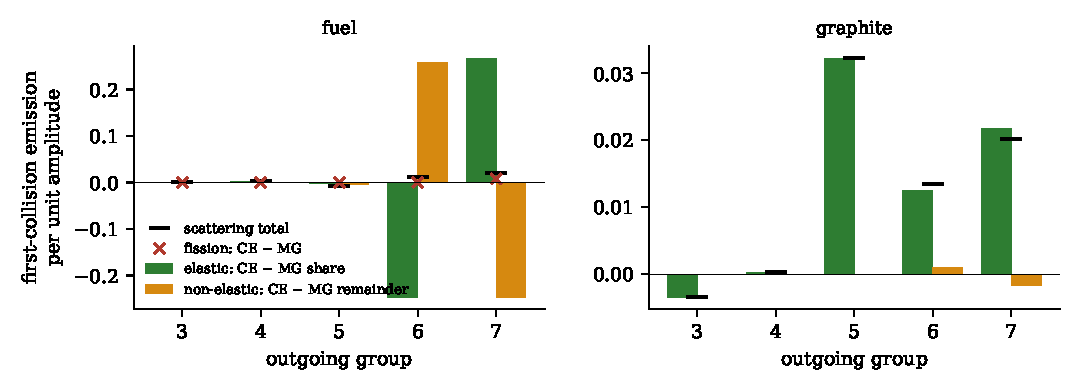
\includegraphics[width=0.92\textwidth]{figures/continuous_channels.pdf}
\caption{First-collision emission, CE minus multigroup, by outgoing group and channel class. The
multigroup matrix holds inelastic scattering; split by one elastic share per incident group, the
elastic and non-elastic parts of the fuel's fast groups differ by about $0.25$ with opposite signs,
and their sum is small.}\label{fig:cont:channels}
\end{figure}

\paragraph{The measure.} One generation's importance-weighted residual, with the importance tabulated
by field region and 60 energy bins, split into a \emph{bin part} (the residual's bin totals times the
bins' mean importance) and a \emph{within-bin part} (the rest), as noise per root second. The split
reproduces the ordering of the eigenvalue figures of merit: the control variate of
Section~\ref{sec:res:bcv} has bin part $0.0097$ (forward bins) and within-bin part $0.024$ (backward
records), $85\%$ of its variance (Figure~\ref{fig:cont:cvbins}).

\begin{figure}[t]\centering
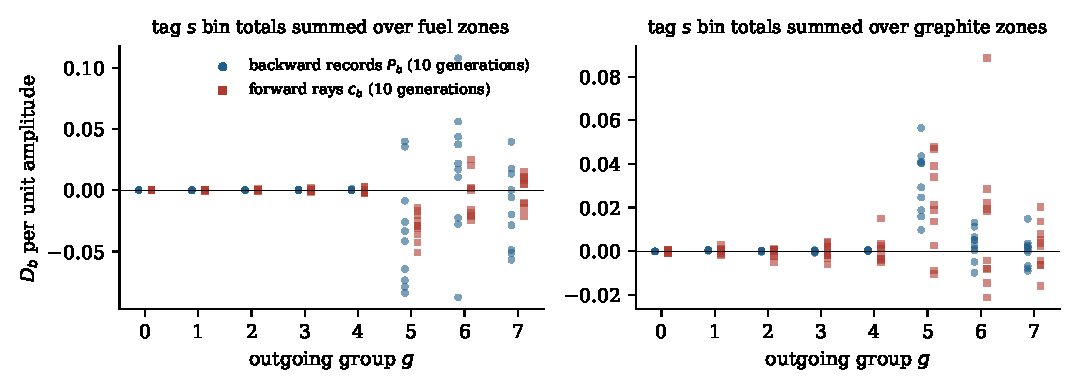
\includegraphics[width=0.92\textwidth]{figures/continuous_cv_bins.pdf}
\caption{Bin totals of the scattering residual's physics part over ten generations: backward records
(blue) and forward rays (red), summed over the zones of each material.}\label{fig:cont:cvbins}
\end{figure}

\paragraph{Partners.} The ray-wise mismatch $\rho=\E\!\int|k_{CE}-k_0|/\E\!\int k_{CE}$ sets the weights:
\begin{center}\footnotesize
\begin{tabular}{@{}lccc@{}}
\toprule
partner & lanes or bands & $\rho$ elastic & $\rho$ fission\\ \midrule
multigroup & 1 & 0.255 & 0.74\\
CE law applied to the multigroup flux & 1 & 0.125 & 0.153\\
RESOLVE lanes, generic starting block with the field's lifts & 64 & 0.017 & 0.033\\
RESOLVE lanes, starting block tuned to the problem & 32 & 0.002 & 0.003\\
bands (subgroup limit), $\log\Sigma_t$ levels, $128\times16$ & 2048 & 0.012 & 0.018\\
\bottomrule
\end{tabular}
\end{center}
The multigroup partner's floor is the in-group attenuation along the ray; RESOLVE lanes remove it.
Truncating the partner's angular law to P$_1$, P$_3$ or P$_7$ leaves $0.11$, $0.08$, $0.065$.

\paragraph{Bounded weights.} With the CE and multigroup proposals alone, $90\%$ of the variance sat in
$0.1\%$ of the samples, at the $^{238}$U resonance minima where the partner and CE disagree and neither
proposal puts mass. A third component drawn from a band library (band by source mass, collision with
the band's $\Sigma_t$, incident energy by $\Sigma_{el}$ within the band) bounds the weights of a band
partner. RESOLVE lanes ring with both signs at the resonance peaks and keep their tails.

\paragraph{Noise.} Scattering, per root second (total; within-bin): multigroup partner $0.119$; $0.028$;
band partner $128\times16$ with the band proposal $0.0064$; $0.0025$, at 20~$\mu$s per sample. Fission
with that partner: $0.0018$ (backward records $0.0098$).

\paragraph{The closure.} The partner's expectation must be added back. Its bin totals come from a band
first-flight sweep (\code{rmc.band\_sweep}: long random rays carry the uncollided flux in every band,
the local part of each segment integral replaced by its exact expectation) and elastic transfer
tables. Gate G8.17 checks them against the partner's own forward points. Its noise per root second is
$0.004$--$0.016$ depending on the number of bands, so that points plus closure total about $0.018$
($32\times16$ bands), against $0.034$ for the control variate: about $3.6$ times in variance $\times$
time, from one generation; the eigenvalue is not yet measured.

\paragraph{What remains.} With the multigroup field, the closure also has structure inside the bins
(the partner's exact-kinematics emission against the multigroup lift), which the points do not carry.
A band field, the band fluxes times tabulated CE emission spectra, removes the energy part; what
remains is the flat-source and angular structure, as for any low order.

\subsection{What optimization could recover}\label{sec:s8:projection}

\begin{table}[t]\centering\small
\caption{Time per generation of the tuned combined variant (single thread), and the projected
speedup of each kernel.}\label{tab:impl:time}
\begin{tabular}{@{}lrrrl@{}}
\toprule
kernel & s/gen & share & projected $\times$ & reason\\
\midrule
residual sampling & 1.55 & 49\% & 4 & total-only lookups, per-path XS cache, channel sampling\\
flights & 0.52 & 16\% & 1.5 & already OpenMC's own collision physics; bank I/O only\\
cancellation & 0.32 & 10\% & 5 & Python loops and \code{numpy} netting moved to C++\\
tallies and bookkeeping & 0.78 & 25\% & 5 & closed-form MG low, C++ bank handling\\
\midrule
total & 3.17 & & 3.3 & \\
\bottomrule
\end{tabular}
\end{table}

\paragraph{Engineering.} Table~\ref{tab:impl:time} splits a generation by kernel.

Residual sampling dominates, and within it the cross-section lookups on backward segments
(Section~\ref{sec:impl:projection}). Each lookup is a full \code{Material::calculate\_xs}, while the
backward flux needs only $\Sigma_t$. A total-only lookup with a per-path cache would remove most of
that cost.

The Python-side cancellation and tally costs are pure overhead.

The flights are OpenMC's own transport and gain little. With the per-kernel factors of the table, a
generation becomes $3.3$ times faster. The $k$ figure of merit would then be $0.07$ (batch means) or
$0.005$ (replicas) of the reference: still at least $15$ times worse than analog Monte Carlo.

\paragraph{Algorithm.} Engineering cannot close that gap, so the remaining factors must come from
the algorithm. The follow-up of Section~\ref{sec:res:followup} narrows down which ones matter.
\begin{enumerate}
\item \textbf{Less noise per residual sample.} This is the dominant lever. The scattering residual
  injects about 7 units of absolute weight per generation, almost all of it integration noise of the
  high term. The candidates are:
  \begin{itemize}
  \item stratified or randomized quasi-Monte Carlo incident directions;
  \item importance-sampled incident energies;
  \item a CE/MG control evaluated on the same incident energies, so that the difference is
    pointwise residual-scale.
  \end{itemize}
  More samples per generation help in the same way: at $N=16000$, $\Wabs$ falls to $1.8$ and the
  figure of merit rises by about two even before optimization (Table~\ref{tab:fu}). Cheaper samples
  (Table~\ref{tab:impl:time}) therefore pay twice.
\item \textbf{Lower $\Wabs$ at fixed noise.} Following amplitudes ($b=a$) remove the production-scale
  amplitude term (21\% lower $\Wabs$). Pooling of scattering children at birth against a shared
  slowing-down density is the remaining exact option.
\item \textbf{Not the correlation.} In neutron lifetimes the collision iteration is already less
  correlated than analog Monte Carlo. Fission-to-fission generations cost more than they save
  (Section~\ref{sec:res:followup}).
\end{enumerate}

\paragraph{Projection to a light-water pincell.} The answer above is for graphite. For a typical PWR
pincell (UO$_2$, water, pitch 1.26~cm), the changes are as follows.
\begin{itemize}
\item \textbf{Reference cost.} A history takes $\approx20$ collisions to thermalize in hydrogen
  ($\xi\approx0.93$), against $\approx115$ in carbon. The reference therefore runs $\approx4$--$5$
  times faster per history.
\item \textbf{RMC cost.} The RMC generation is one collision generation, so its cost per generation
  is unchanged.
\item \textbf{Correlation.} The scattering modes decay as $c^n$ with $c$ lower in a hydrogenous
  pincell (more absorption per collision near the fuel), so the correlation time shortens by a
  similar factor.
\item \textbf{Residual.} The MG field is a worse approximation in an LWR: harder spectrum, stronger
  $^{238}$U self-shielding, more epithermal fission. This raises $V_{res}$ and $\Wabs$.
\end{itemize}
The net is roughly neutral to unfavourable. The LWR figure of merit ratio should be no better than
the graphite one, and plausibly 2--3 times worse unless the MG field carries self-shielded
cross sections.

\subsection{Verdict}

The method runs, and after Sections~\ref{sec:res:speedup} and~\ref{sec:res:lifts} it is unbiased
within the present precision:
\begin{itemize}
\item \textbf{Bias.} With lifts that resolve the resonances, the eigenvalue bias is $-86\pm58$~pcm
  (nine replicas), down from $+650$ to $+1000$~pcm. Its cause was netting acting on the unresolved
  resonance structure of the low term.
\item \textbf{The correction.} The scattering residual is about 15 times more efficient than in the
  first measurement (proposal, tracer, several energies per trace, lifts). The bank's absolute
  weight is below the fission production ($\Wabs\approx0.85$), from 4.4.
\item \textbf{Figure of merit.} With the binned control variate of Section~\ref{sec:res:bcv}, whose
  residual is unbiased, it is $1$--$2$ times analog Monte Carlo's for $k$ on the spread of six
  replicas and $2$--$3$ on batch means; with residual samples from backward points it was about
  $0.4$. A biased form that holds the residual only in the netting bins reached $5.5$
  (Section~\ref{sec:res:correlated}). Pointwise forward points with a band partner and its closure
  project to about $3.6$ times the control variate (Section~\ref{sec:res:continuous}).
\end{itemize}

What limits it has changed three times. It is no longer the scattering residual, no longer the
field's fission production $X$ (Section~\ref{sec:res:X}), and no longer the eigenvalue update, whose
lifetime-long memory the balance estimate removes. Exact grouped cancellation at fission births is
implemented and verified, but it is not sufficient for weight cancellation: the weight that must
cancel is scattering weight, and netting remains necessary. The next stage should:
\begin{enumerate}
\item test a problem with fewer collisions per neutron lifetime (a water lattice or a fast system):
  a coarser mesh, a better loss estimator and a resonance-resolving low order have all left the
  figure of merit where it was on the graphite pincell (Section~\ref{sec:res:forward});
\item build a single-generation efficiency measure that includes netting, so that the sampler can be
  tuned again; and find the origin of the bias of $-10$ to $-50$~pcm.
\end{enumerate}


\part{Nuclear data}\label{part:nd}

The method touches nuclear data in three places: the CE cross sections that attenuate backward
paths and flights, the production kernels whose densities the evaluators compute, and the collision
routines the sampler route and the flights call. This part starts from the physics of individual
reactions, follows them into the evaluated files and OpenMC's library, shows how they shape the
spectra of a real lattice, and ends with what each reaction means for this method.

\section{Reactions and cross sections}\label{sec:nd:reactions}

\subsection{What a cross section is}

A \textbf{microscopic cross section} $\sigma_x(E)$ is the effective area a nucleus presents to a
neutron of energy $E$ for reaction $x$; its unit is the barn ($10^{-24}$ cm$^2$). The probability of
reaction $x$ per unit path in a material with atom densities $N_i$ is the macroscopic cross section
$\Sigma_x=\sum_iN_i\sigma_{x,i}$ (cm$^{-1}$). The total cross section is the sum over all reactions;
the mean free path is $1/\Sigma_t$. Reactions are identified by ENDF \textbf{MT} numbers: 1 total, 2
elastic, 4 inelastic (sum of 51--91), 16 $(n,2n)$, 18 fission, 51--90 inelastic to discrete levels,
91 inelastic continuum, 102 radiative capture $(n,\gamma)$, 103--107 charged-particle emission.

\subsection{The reactions that matter for neutron transport}

\begin{itemize}
\item \textbf{Elastic scattering} (MT 2) conserves kinetic energy in the centre-of-mass frame; the
  neutron loses energy to the recoiling nucleus. It dominates in moderators and at most energies in
  fuel. It has a potential part (hard-sphere, smooth) and resonance parts.
\item \textbf{Inelastic scattering} (MT 51--91) leaves the nucleus excited. To a discrete level
  (MT 51--90) the Q-value $-Q$ is fixed and the kinematics are two-body; above the highest resolved
  level the continuum (MT 91) is described statistically. Thresholds lie near $|Q|(A+1)/A$; for U-238
  the first level is at 45 keV.
\item \textbf{$(n,xn)$} reactions emit several neutrons; the yield multiplies the production.
\item \textbf{Fission} (MT 18, or partial MT 19--21, 38 for first, second, third and fourth
  chance) emits on average $\bar\nu(E)$ neutrons, prompt and delayed, with an energy spectrum $\chi$
  peaked near 1 MeV.
\item \textbf{Capture} (MT 102) removes the neutron; it matters through $\Sigma_t$ and self-shielding.
\end{itemize}

\begin{figure}[t]\centering
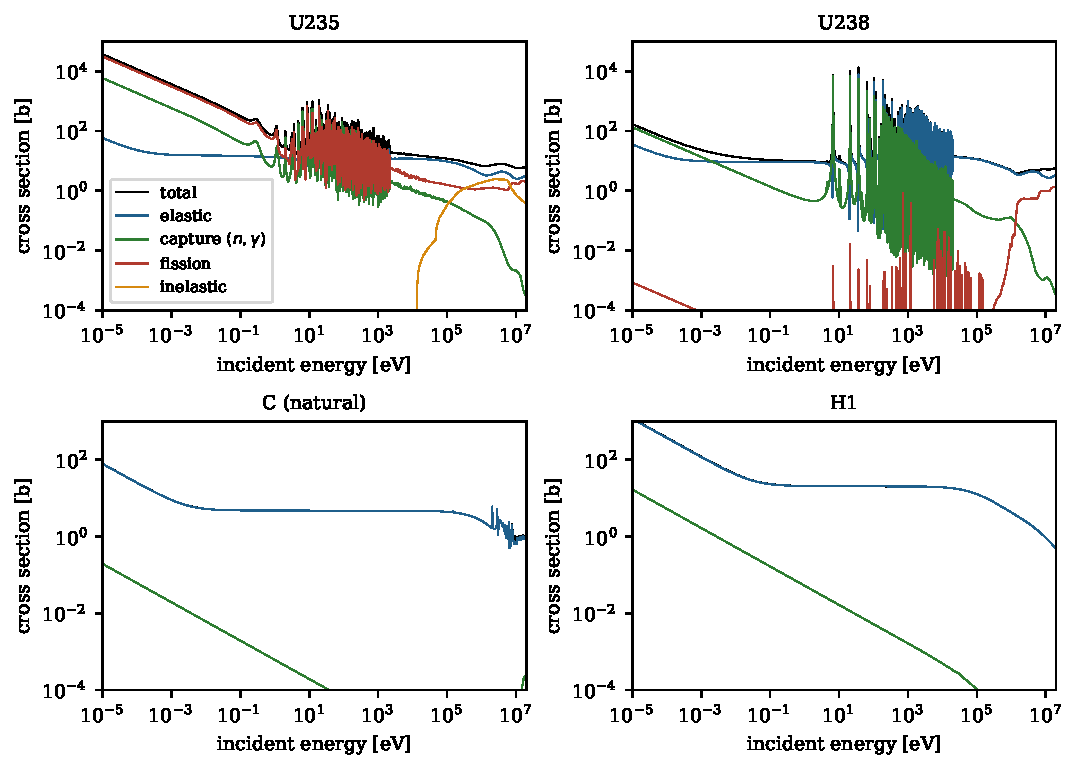
\includegraphics[width=\textwidth]{figures/nd_cross_sections.pdf}
\caption{Cross sections at 294 K from the library used here. U-235: the $1/v$ fission and capture at
low energy, the resolved resonances from 1 eV to 2.25 keV, and smooth fast data. U-238: giant capture
resonances (6.67, 20.9, 36.7 eV, \dots), the inelastic threshold at 45 keV and the fission threshold
near 1 MeV. Carbon: nearly constant elastic scattering up to MeV, then resonances. Hydrogen: elastic
only (plus a small capture), flat to 10 keV.}\label{fig:nd:xs}
\end{figure}

\subsection{Energy ranges}

The data of a heavy nuclide fall into four ranges (Figure~\ref{fig:nd:xs}): the \emph{thermal} range
($\lesssim1$ eV), where cross sections often follow $1/v$ and the target's thermal motion and
chemical binding matter; the \emph{resolved resonance} range, where individual compound-nucleus
states appear as Breit--Wigner or R-matrix resonances; the \emph{unresolved resonance} range, where
resonances overlap in the data but not in nature and are described statistically; and the
\emph{fast} range, smooth and dominated by elastic, inelastic and fission.

\section{Representations and formats}\label{sec:nd:formats}

\subsection{Evaluated data: ENDF-6}

Evaluations (ENDF/B, JEFF, JENDL) are distributed in the ENDF-6 format, organized by \emph{files}
(MF) and \emph{sections} (MT). MF 2 holds resonance parameters, MF 3 smooth cross sections, MF 4
angular distributions, MF 5 energy distributions, MF 6 correlated energy--angle distributions, MF 1
$\bar\nu$ and delayed-neutron data, MF 7 thermal scattering laws. Evaluations are not directly
usable for transport: resonances must be reconstructed into pointwise data, Doppler broadened to the
temperature of interest, and thermal laws converted to tables. NJOY does this processing.

\subsection{Processed data: ACE and OpenMC's HDF5}

NJOY writes ACE files; OpenMC converts them into its own HDF5 format (\code{openmc.data}), which
holds per nuclide:
\begin{itemize}
\item a union energy grid per temperature, with cross sections of each reaction on it,
  linear--linear interpolable (the grid is chosen so that interpolation error is below a tolerance);
\item for each reaction its Q-value, its threshold index and its \emph{products}: particle type,
  yield (constant, tabulated in $E$, or polynomial; $\bar\nu$ for fission), emission mode (prompt
  or delayed with its decay constant), and a list of distributions with applicability weights;
\item unresolved-resonance probability tables (optional), and windowed multipole data for
  on-the-fly Doppler broadening (optional).
\end{itemize}
Thermal scattering data S($\alpha,\beta$) are separate files for a material (e.g.\ H in H$_2$O,
graphite).

\subsection{Resonances, Doppler broadening and unresolved resonances}

\textbf{Resolved resonances.} Near an isolated compound-nucleus state of energy $E_0$ the
single-level Breit--Wigner form gives
\begin{equation}
\sigma_\gamma(E)=\sigma_0\frac{\Gamma_\gamma}{\Gamma}\sqrt{\frac{E_0}{E}}\frac{1}{1+x^2},\qquad
\sigma_n(E)=\sigma_0\frac{\Gamma_n}{\Gamma}\frac{1}{1+x^2}+\sigma_0\frac{2R}{\bar\lambda_0}\frac{x}{1+x^2}+4\pi R^2,
\qquad x=\frac{2(E-E_0)}{\Gamma},
\end{equation}
with partial widths $\Gamma_n,\Gamma_\gamma$, total width $\Gamma$, peak $\sigma_0$, reduced wavelength $\bar\lambda_0$ at $E_0$ and channel radius
$R$; the middle term of $\sigma_n$ is the interference between resonance and potential scattering,
which produces the characteristic dip below each elastic resonance. Evaluations use multilevel
Breit--Wigner or Reich--Moore R-matrix forms, which NJOY reconstructs into pointwise data.

\textbf{Doppler broadening.} The target nuclei move thermally, so the cross section seen by a neutron
of lab energy $E$ is an average over relative speeds,
\begin{equation}
\bar\sigma(E,T)=\frac{1}{v^2}\sqrt{\frac{\beta}{\pi}}\int_0^\infty v_r^2\,\sigma(v_r)
\Big[e^{-\beta(v_r-v)^2}-e^{-\beta(v_r+v)^2}\Big]\dd v_r,\qquad\beta=\frac{AM_n}{2kT},
\end{equation}
which lowers and widens resonances at higher temperature while preserving their area. Processed
libraries tabulate it at a few temperatures; OpenMC interpolates between them or evaluates windowed
multipole representations on the fly.

\textbf{Unresolved resonances.} Above the resolved range the evaluation gives only average resonance
parameters. Probability tables represent the distribution of the cross section at each energy: a
particle samples a band once per energy and uses it consistently. A backward trace cannot simply use
the mean, because the expected transmission $\E[e^{-\Sigma\ell}]$ differs from $e^{-\E[\Sigma]\ell}$;
probability tables are therefore off in the verification problems here.

\begin{figure}[t]\centering
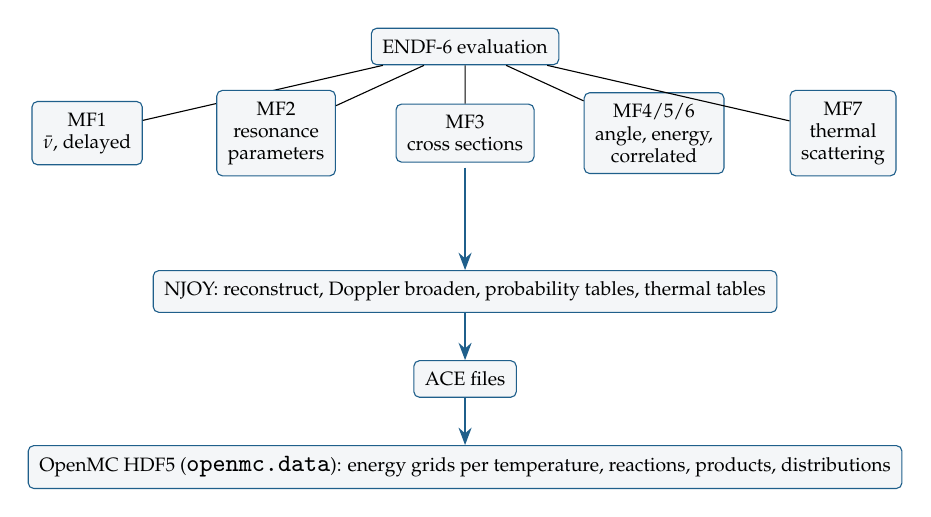
\begin{tikzpicture}[level distance=11mm, sibling distance=24mm, every node/.style={box,font=\scriptsize}]
\node (endf) {ENDF-6 evaluation}
  child {node {MF1\\ $\bar\nu$, delayed}}
  child {node {MF2\\ resonance\\ parameters}}
  child {node {MF3\\ cross sections}}
  child {node {MF4/5/6\\ angle, energy,\\ correlated}}
  child {node {MF7\\ thermal\\ scattering}};
\node[below=26mm of endf] (njoy) {NJOY: reconstruct, Doppler broaden, probability tables, thermal tables};
\node[below=6mm of njoy] (ace) {ACE files};
\node[below=6mm of ace] (h5) {OpenMC HDF5 (\code{openmc.data}): energy grids per temperature, reactions, products, distributions};
\draw[arr] ([yshift=-13mm]endf.south) -- (njoy.north);
\draw[arr] (njoy) -- (ace);
\draw[arr] (ace) -- (h5);
\end{tikzpicture}
\caption{From evaluation to OpenMC's library.}\label{fig:nd:pipeline}
\end{figure}

\subsection{Energy grids and lookups}

Each nuclide's cross sections are tabulated on its own energy grid, linear--linear between points.
A lookup at energy $E$ needs the grid index for every nuclide in the material; OpenMC uses a
logarithmic hash: a uniform grid in $\ln E$ maps $E$ to a small index range of each nuclide's grid,
where a binary search finishes. The macroscopic total is then a sum over the material's nuclides.
This is the operation the backward characteristic performs once per segment and energy, which is
why it dominates the cost (Part~\ref{part:impl}).

\subsection{Secondary distributions}

The outgoing state of a reaction is described in one of three ways.

\textbf{Uncorrelated angle--energy.} Angle and energy are independent: an angular distribution
$p(\mu\mid E')$ (Legendre series or tabulated, usually in the CM frame) and an energy distribution
$f(E\mid E')$ given by one of the ENDF \emph{laws}:
\begin{itemize}
\item \emph{continuous tabular} (law 4 / ACE law 4): $f(E\mid E'_\ell)$ tabulated at incident grid
  points, histogram or linear in $E$, with a stochastic choice between neighbouring incident tables and
  a rescaling of the outgoing range (``unit-base interpolation'');
\item \emph{Maxwell} $f\propto\sqrt E\,e^{-E/\theta(E')}$, \emph{evaporation}
  $f\propto E\,e^{-E/\theta(E')}$, \emph{Watt} $f\propto e^{-E/a}\sinh\sqrt{bE}$, each restricted to
  $E\le E'-U$;
\item \emph{discrete photon / level} (law 3): inelastic to a level; the outgoing energy follows from
  two-body kinematics and the angle.
\end{itemize}

\textbf{Correlated angle--energy.} Kalbach--Mann systematics (law 44) give
$p(\mu\mid E,E')=\frac{a}{2\sinh a}[\cosh(a\mu)+r\sinh(a\mu)]$ with tabulated $r(E,E')$ and a
closed-form $a$; law 61 tabulates angular distributions per outgoing energy; N-body phase space (law
66) is closed-form.

\textbf{Thermal scattering S($\alpha,\beta$).} Below a few eV the target's binding and motion are
described by the scattering law $S(\alpha,\beta)$ in momentum transfer $\alpha$ and energy transfer
$\beta$. Processed data give incoherent inelastic scattering as discrete outgoing energies and angles
(or continuous tables), coherent elastic scattering as Bragg edges (scattering only at discrete
cosines per lattice plane), and incoherent elastic scattering (for hydrogen in metal hydrides).

\subsection{Fission data}

$\bar\nu(E)$ is the sum of prompt $\bar\nu_p$ and delayed $\bar\nu_d$ (six or eight precursor groups
with decay constants and spectra). The prompt spectrum depends weakly on the incident energy
(Figure~\ref{fig:nd:fission}); for U-235 and U-238 it is tabulated (law 4), for minor actinides often
Watt or Maxwell. Second- and third-chance fission (partial MTs) have their own spectra.

\begin{figure}[t]\centering
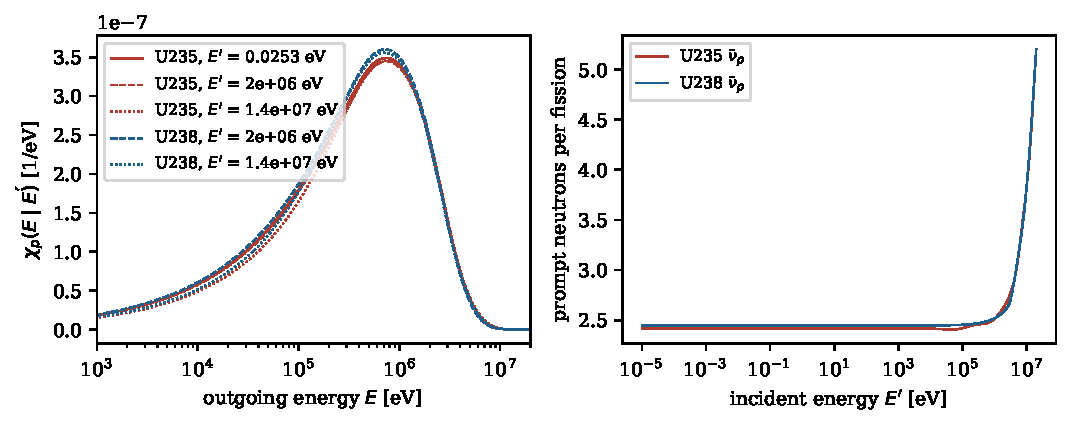
\includegraphics[width=\textwidth]{figures/nd_fission.pdf}
\caption{Left: prompt fission spectra of U-235 and U-238 at several incident energies: nearly the
same shape, peaked near 1 MeV, harder at high incident energy. Right: prompt $\bar\nu$ against incident
energy: flat below 1 MeV, rising linearly above, with steps at the second-chance threshold.}\label{fig:nd:fission}
\end{figure}

\section{How the data shape a reactor spectrum}\label{sec:nd:physics}

\subsection{Slowing down}

Fission neutrons are born near 2 MeV and are absorbed mostly below 1 eV, so they must lose six to
eight decades of energy. Elastic scattering off a nucleus at rest of mass ratio $A$ leaves a fraction
of the energy between $\alpha=((A-1)/(A+1))^2$ and 1; for isotropic CM scattering the ratio $E/E'$
is uniform on $[\alpha,1]$ (Figure~\ref{fig:nd:elastic}). The average lethargy gain per collision is
\begin{equation}
\xi=1+\frac{\alpha\ln\alpha}{1-\alpha}\approx\frac{2}{A+2/3},
\end{equation}
1 for hydrogen, 0.158 for carbon, 0.0084 for U-238: a neutron needs about 20 collisions in water
($\xi\approx0.92$) and 115 in graphite to slow from 2 MeV to thermal energies. In an infinite medium with constant scattering and no
absorption, the flux between the source and thermal energies is $\phi(E)\propto1/(\xi\Sigma_sE)$:
flat per unit lethargy, the $1/E$ spectrum visible in Figure~\ref{fig:nd:spectrum}.

\begin{figure}[t]\centering
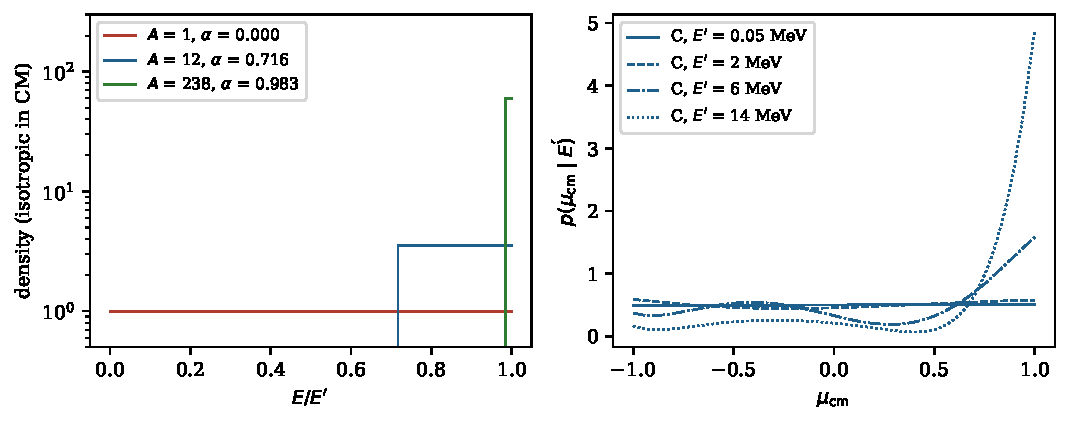
\includegraphics[width=\textwidth]{figures/nd_elastic.pdf}
\caption{Left: energy after one elastic collision with isotropic CM scattering, for $A=1$, 12 and
238. Right: CM angular distribution of elastic scattering on carbon: isotropic at 100 keV,
increasingly forward-peaked at MeV energies. Forward-peaked scattering is what the P$_0$ MG control
cannot represent.}\label{fig:nd:elastic}
\end{figure}

\begin{figure}[t]\centering
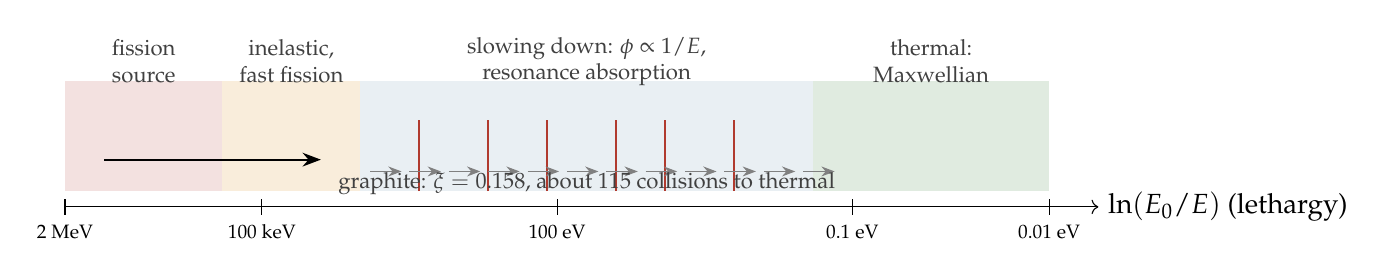
\begin{tikzpicture}[xscale=1.25]
\draw[->] (0,0) -- (10.5,0) node[right] {$\ln(E_0/E)$ (lethargy)};
\foreach \x/\l in {0/2 MeV,2/100 keV,5/100 eV,8/0.1 eV,10/0.01 eV} {\draw (\x,0.1)--(\x,-0.1) node[below,font=\scriptsize] {\l};}
\fill[accred!15] (0,0.2) rectangle (1.6,1.6); \node[note] at (0.8,1.85) {fission\\ source};
\fill[accorange!15] (1.6,0.2) rectangle (3,1.6); \node[note] at (2.3,1.85) {inelastic,\\ fast fission};
\fill[headblue!10] (3,0.2) rectangle (7.6,1.6); \node[note] at (5.3,1.85) {slowing down: $\phi\propto1/E$,\\ resonance absorption};
\fill[accgreen!15] (7.6,0.2) rectangle (10,1.6); \node[note] at (8.8,1.85) {thermal:\\ Maxwellian};
\foreach \x in {3.6,4.3,4.9,5.6,6.1,6.8} \draw[thick,accred] (\x,0.2) -- (\x,1.1);
\draw[-{Stealth},thick] (0.4,0.6) -- (1.1,0.6) -- (1.5,0.6) -- (2.2,0.6) -- (2.6,0.6);
\foreach \x in {3.1,3.5,3.9,4.3,4.7,5.1,5.5,5.9,6.3,6.7,7.1,7.5} \draw[-{Stealth},gray] (\x,0.45) -- ++(0.32,0);
\node[note] at (5.3,0.3) {graphite: $\xi=0.158$, about 115 collisions to thermal};
\end{tikzpicture}
\caption{The life of a neutron in lethargy. Fission emits at MeV energies; inelastic scattering and fast
fission act above 100 keV; elastic collisions move the neutron through the resonance range in steps of
$\xi$, where U-238 resonances (red) absorb; below about 1 eV the neutron thermalizes.}\label{fig:nd:cascade}
\end{figure}

\subsection{Resonance absorption and self-shielding}

As neutrons slow down past the U-238 resonances, the flux in the fuel dips sharply at each resonance:
the fuel absorbs so strongly at the resonance energy that the interior of the pin sees fewer neutrons
(\emph{spatial self-shielding}), and the flux depression in energy reduces the effective capture
(\emph{energy self-shielding}). Figure~\ref{fig:nd:resonances} shows both: the fuel's flux falls at
each resonance, and the graphite's falls too, since fewer neutrons at those energies leave the
fuel. A multigroup model must average these dips into a group constant; the averaging is done with a
weighting spectrum that is right only for the problem it came from. This is the dominant source of
the MG field's error and therefore of the residual (Section~\ref{sec:res:controlled}).

\begin{figure}[t]\centering
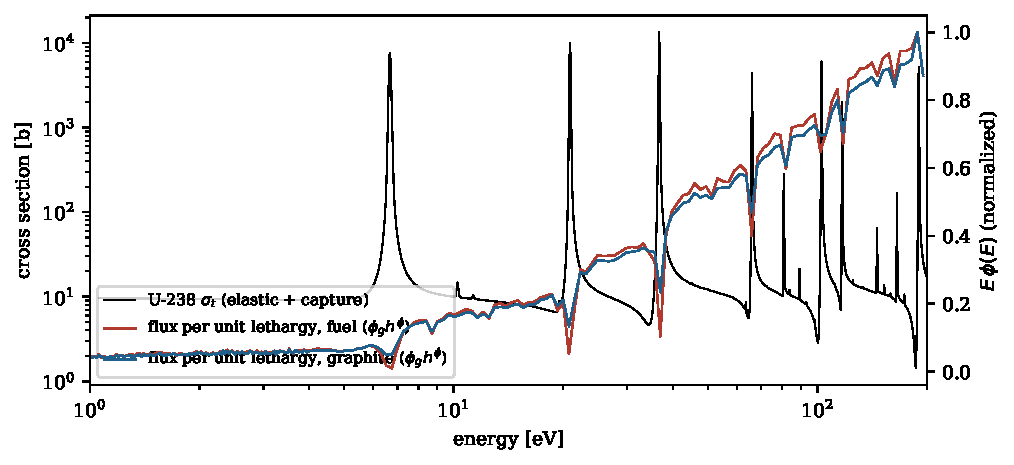
\includegraphics[width=\textwidth]{figures/nd_resonances.pdf}
\caption{U-238 resonances and the flux per unit lethargy in the fuel and graphite of the pincell
(from the CE lift tallies). The flux dips at every resonance; the group boundaries of CASMO-8 lie at
4 eV and 5.53 keV, so a single group must average across all of these structures.}\label{fig:nd:resonances}
\end{figure}

\subsection{Thermalization}

Below about 1 eV the neutron's energy is comparable to the target's thermal motion, so collisions can
\emph{raise} the energy. The flux tends to a Maxwellian
$\phi(E)\propto E\,e^{-E/kT}$, hardened by absorption. Free-atom (free-gas) scattering treats the
target as a gas at temperature $T$; chemical binding (S($\alpha,\beta$)) changes the exchange
of energy, most strongly for hydrogen in water and for graphite.

\begin{figure}[t]\centering
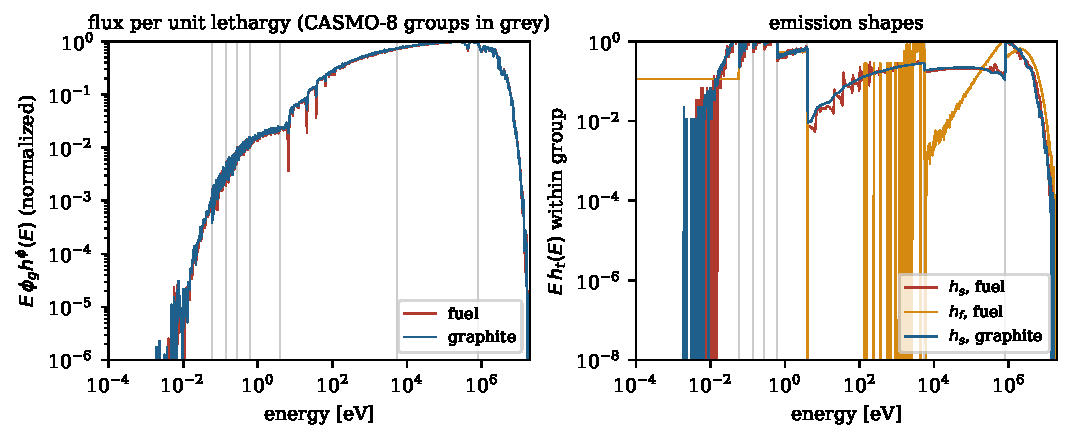
\includegraphics[width=\textwidth]{figures/nd_spectrum_lifts.pdf}
\caption{The graphite pincell's spectrum. Left: flux per unit lethargy in fuel and graphite, showing
the fission source above 100 keV, the $1/E$ slowing-down plateau with resonance dips, and the thermal
range. Right: the emission shapes the lifts carry within each group.}\label{fig:nd:spectrum}
\end{figure}

\begin{figure}[t]\centering
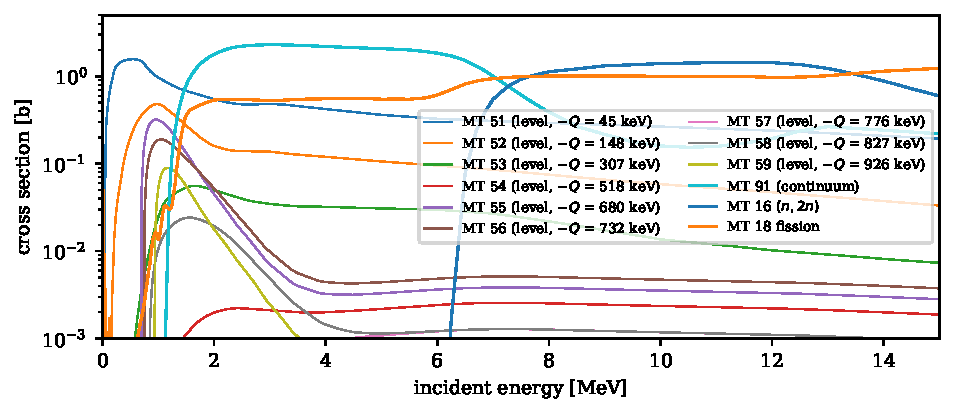
\includegraphics[width=\textwidth]{figures/nd_inelastic.pdf}
\caption{U-238 inelastic scattering to discrete levels (thresholds at 45, 148, \dots\ keV),
continuum, $(n,2n)$ and fission. Inelastic scattering moves neutrons from MeV to tens of keV in one
collision.}\label{fig:nd:inelastic}
\end{figure}

\section{How OpenMC samples each reaction}\label{sec:nd:openmc}

\subsection{The collision}

OpenMC's \code{collision()} (in \code{src/physics.cpp}) is entered at a collision site with the
particle's macroscopic and microscopic cross sections already computed by
\code{Material::calculate\_xs} at the particle's energy and temperature (with probability tables,
S($\alpha,\beta$) and multipole data where enabled). It proceeds:

\begin{algorithm}[h]
\caption{OpenMC's analog neutron collision (simplified)}
\DontPrintSemicolon
choose nuclide $m$ with probability $N_m\sigma_{t,m}/\Sigma_t$ \tcp*{\code{sample\_nuclide}}
\eIf{$\xi<\sigma_{s,m}/\sigma_{t,m}$}{scatter: \code{scatter(p, m)}}{
  absorption: create fission sites with expected count $w\,\nu\sigma_f/(k\,\sigma_t)$ (eigenvalue)\;
  survival biasing or analog kill\;
}
\end{algorithm}

\code{scatter()} chooses between elastic (with S($\alpha,\beta$) below its cutoff) and the other
scattering reactions by their cross sections, then calls:
\begin{itemize}
\item \textbf{\code{elastic\_scatter}}: samples a target velocity (\code{sample\_target\_velocity}):
  at rest if $A>1$ and $E\ge$ \code{free\_gas\_threshold}$\cdot kT$ (and the nuclide is not a
  resonant scatterer); otherwise a free-gas Maxwellian with the constant-cross-section approximation,
  or DBRC/RVS for resonant scatterers. It transforms to the CM frame, samples $\mu_{cm}$ from the
  angular distribution, rotates and transforms back.
\item \textbf{\code{sab\_scatter}}: samples from the S($\alpha,\beta$) tables (coherent elastic: a
  Bragg edge, then the cosine it implies; incoherent: discrete or continuous tables).
\item \textbf{\code{inelastic\_scatter}}: samples the product's distribution (\code{ReactionProduct::sample}),
  converts CM to lab where needed, and handles the yield: a fractional yield multiplies the weight,
  an integer yield $\nu>1$ banks $\nu-1$ copies with the \emph{same} outgoing state.
\end{itemize}
Fission (\code{create\_fission\_sites}) samples the reaction among partial fission reactions by
cross section (\code{sample\_fission}) and each neutron with \code{sample\_fission\_neutron}: prompt
or delayed by $\bar\nu_d/\bar\nu$, the delayed group by its yield, then the energy from the
corresponding distribution, resampled until $E<E_{max}$ of the data; isotropic direction.

\subsection{The sampling algorithms of the energy laws}

\begin{algorithm}[h]
\caption{Continuous tabular energy law (ENDF law 4 / ACE law 4), as in OpenMC}\label{alg:law4}
\DontPrintSemicolon
find $\ell$ with $E'_\ell\le E'<E'_{\ell+1}$; $r\gets(E'-E'_\ell)/(E'_{\ell+1}-E'_\ell)$ (log-log in some data)\;
$i\gets\ell+1$ with probability $r$, else $i\gets\ell$ \tcp*{stochastic interpolation}
sample $\hat E$ from table $i$ (histogram or linear-linear CDF inversion; discrete lines first)\;
$E_{lo}\gets(1-r)E^{(\ell)}_{min}+rE^{(\ell+1)}_{min}$;\quad $E_{hi}$ likewise\;
$E\gets E_{lo}+(\hat E-E^{(i)}_{min})\frac{E_{hi}-E_{lo}}{E^{(i)}_{max}-E^{(i)}_{min}}$\tcp*{unit-base rescaling}
\end{algorithm}

Its density is therefore a mixture of the two tables, each mapped onto the interpolated range with the
Jacobian $(E^{(i)}_{max}-E^{(i)}_{min})/(E_{hi}-E_{lo})$ (Section~\ref{sec:nd:openmc}). The other laws:
\begin{itemize}
\item \textbf{Maxwell} $f\propto\sqrt E\,e^{-E/\theta}$: sampled as $-\theta(\ln\xi_1+\ln\xi_2\cos^2(\pi\xi_3/2))$
  and rejected until $E\le E'-U$; its density is the Maxwellian renormalized to $[0,E'-U]$.
\item \textbf{Watt} $f\propto e^{-E/a}\sinh\sqrt{bE}$: sampled from a Maxwellian of temperature $a$ and a
  shift, $E=w+\frac{a^2b}{4}+(2\xi-1)\sqrt{a^2bw}$, with rejection on $[0,E'-U]$.
\item \textbf{Evaporation} $f\propto E\,e^{-E/\theta}$: by inversion of a gamma distribution, rejected on
  $[0,E'-U]$.
\item \textbf{Kalbach--Mann}: $E$ from law-4-like tables with tabulated precompound fraction $r$; then
  $\mu$ from $\frac{a}{2\sinh a}(\cosh a\mu+r\sinh a\mu)$ by a two-branch inversion.
\end{itemize}

\subsection{Free-gas elastic scattering in OpenMC}

Below the free-gas threshold (or for resonant scatterers), OpenMC samples a target velocity from the
distribution $P(\mathbf V)\propto|\mathbf v-\mathbf V|\,\sigma(|\mathbf v-\mathbf V|)\,M(\mathbf V)$, with
$M$ the Maxwellian at the material temperature. With constant $\sigma$ this is done by sampling the
target speed from a mixture of $V^3e^{-\beta V^2}$ and $V^2e^{-\beta V^2}$ and the cosine between target and
neutron with rejection on the relative speed. The neutron then scatters isotropically (or with the
tabulated CM distribution) in the CM frame of the pair. The exact density of this procedure is the
free-gas kernel above; the DBRC and RVS options for resonant scatterers replace the constant cross
section by the 0 K resonant one in the rejection step.

\begin{figure}[t]\centering
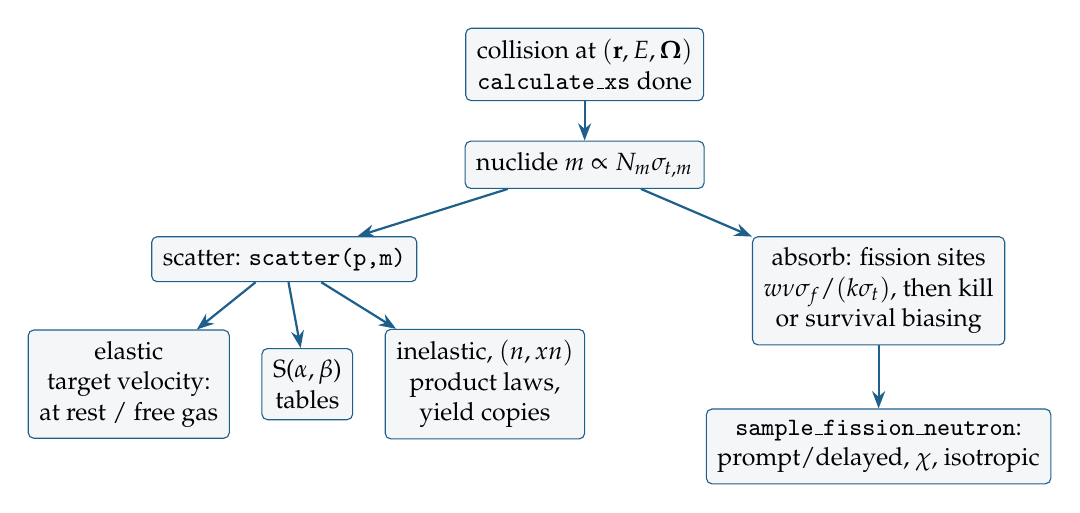
\begin{tikzpicture}[node distance=5mm and 8mm, every node/.style={font=\footnotesize}]
\node[box] (c) {collision at $(\vr,E,\vO)$\\ \code{calculate\_xs} done};
\node[box,below=of c] (nuc) {nuclide $m$ $\propto N_m\sigma_{t,m}$};
\node[box,below left=6mm and 6mm of nuc] (sc) {scatter: \code{scatter(p,m)}};
\node[box,below right=6mm and 6mm of nuc] (ab) {absorb: fission sites\\ $w\nu\sigma_f/(k\sigma_t)$, then kill\\ or survival biasing};
\node[box,below left=6mm and -10mm of sc] (el) {elastic\\ target velocity:\\ at rest / free gas};
\node[box,right=4mm of el] (sab) {S($\alpha,\beta$)\\ tables};
\node[box,right=4mm of sab] (inel) {inelastic, $(n,xn)$\\ product laws,\\ yield copies};
\node[box,below=8mm of ab] (fis) {\code{sample\_fission\_neutron}:\\ prompt/delayed, $\chi$, isotropic};
\draw[arr] (c)--(nuc); \draw[arr] (nuc)--(sc); \draw[arr] (nuc)--(ab);
\draw[arr] (sc)--(el); \draw[arr] (sc)--(sab); \draw[arr] (sc)--(inel); \draw[arr] (ab)--(fis);
\end{tikzpicture}
\caption{OpenMC's analog neutron collision and the routines this method reuses: the sampler route and
the flights call \code{scatter} and \code{sample\_fission\_neutron} on scratch particles.}\label{fig:nd:collision}
\end{figure}

\subsection{What a sampler does that a density must match}

An evaluator is correct only if it is the density of \emph{exactly} what the sampler does. Three
details matter in practice:
\begin{enumerate}
\item \textbf{Stochastic interpolation between incident tables.} For law 4, OpenMC picks table
  $\ell$ or $\ell+1$ with probability $1-r$ and $r$ and then rescales the outgoing energy to
  interpolated endpoints. The density is therefore a mixture of two rescaled tabulated densities,
  each with its Jacobian:
  $f(E\mid E')=(1-r)f_\ell(E_\ell(E))\frac{\dd E_\ell}{\dd E}+rf_{\ell+1}(E_{\ell+1}(E))\frac{\dd E_{\ell+1}}{\dd E}$.
  Without the Jacobian the density is wrong between grid points and right at them.
\item \textbf{Rejection on $E_{max}$} conditions the distribution; the density is renormalized
  accordingly.
\item \textbf{Target motion} below the free-gas threshold turns the elastic kernel from a curve in
  $(E,\mu_0)$ into a two-dimensional density; the stationary image formula no longer applies.
\end{enumerate}

\section{Consequences for this method}\label{sec:nd:consequences}

\subsection{Which reactions have densities today}

\begin{table}[t]\centering\small
\begin{tabularx}{\textwidth}{>{\raggedright}p{3.3cm}>{\raggedright}p{3.6cm}>{\raggedright}p{2.1cm}X}
\toprule
Reaction & OpenMC sampler & Route now & A density from the evaluation\\
\midrule
elastic, stationary target ($A>1$) & CM angle, two-body & evaluator & image formula \eqref{eq:elastic_image} (done)\\
fission, prompt and delayed & law 4 / Maxwell / Watt / evaporation & evaluator & density of the sampler incl.\ interpolation (done)\\
elastic, free gas (H, below threshold) & Maxwellian target & sampler & closed-form free-gas kernel (constant $\sigma$)\\
inelastic to a level (MT 51--90) & CM angle, two-body with $Q$ & sampler & image formula with $Q$: $E'$ from $(E,\mu_0)$, Jacobian\\
continuum (MT 91), law 4 & tabulated & sampler & as fission's law 4 (with angle)\\
Kalbach--Mann (law 44) & tabulated $E$, closed-form $\mu$ & sampler & product of law-4 density and the Kalbach angle density\\
law 61 & tabulated $E$, tabulated $\mu$ & sampler & interpolated tables, same Jacobians\\
$(n,xn)$ & as above, yield & sampler & as above, times the yield\\
S($\alpha,\beta$) incoherent inelastic & discrete or continuous tables & sampler & continuous: interpolation; discrete: mixture of points, not a density\\
S($\alpha,\beta$) coherent elastic & Bragg edges & sampler & discrete cosines: delta functions in $\mu$; an image formula in $E'$ per edge\\
unresolved resonances & probability tables & (off) & $\Sigma_t$ random per particle: $\E e^{-\tau}\ne e^{-\E\tau}$\\
\bottomrule
\end{tabularx}
\caption{Reactions, how OpenMC samples them, their route in this method, and how a density for the
evaluator route could be built from the evaluation.}\label{tab:nd:routes}
\end{table}

Table~\ref{tab:nd:routes} summarizes. Two things decide whether a density is worth building:
\begin{itemize}
\item \textbf{Variance.} An evaluator places the production at the destination's state, where the
  low term cancels it pointwise. On the sampler route the production lands elsewhere, and the low
  term must be cancelled by netting or pooling. The controlled residual study shows that for elastic
  scattering in graphite the density route is 7--10 times more efficient even after the low term is
  made exact; for fission, the sampler route with an exact low term is 5--10 times more efficient.
\item \textbf{Cost.} An evaluator costs a density evaluation per image; images multiply with the
  number of nuclides ($n_E$ grows), while the sampler costs one collision per incident energy.
\end{itemize}

\subsection{Densities from the evaluation, concretely}

\textbf{Discrete inelastic levels} are two-body reactions with $Q<0$. With the same notation as
elastic, the lab outgoing energy is $E=E'\gamma(\mu_0;E',Q)$, now depending on $E'$ through the
threshold factor $\Delta=\sqrt{1+(A+1)Q/(AE')}$; for each $(E,\mu_0)$ there are at most two images
$E'$, found by a one-dimensional root solve, with Jacobian $|\partial E/\partial E'|^{-1}$. The CM
angular density comes from MF 4 exactly as for elastic.

\textbf{Continuum and correlated laws} already have the structure of densities: law 4 tables are
densities in $E$ at each incident grid point; Kalbach--Mann's angular part is closed-form; law 61
tabulates $p(\mu\mid E,E')$. The work is to reproduce OpenMC's interpolation and frame transformation
exactly, as was done for fission.

\textbf{Free-gas elastic scattering} with a constant cross section has a closed-form
double-differential kernel. In the ENDF convention, with $\alpha=(E+E'-2\mu_0\sqrt{EE'})/(AkT)$ and
$\beta=(E-E')/kT$,
\begin{equation}
\frac{\dd^2\sigma}{\dd E\,\dd\mu_0}(E'\to E,\mu_0)=\frac{\sigma_b}{2kT}\sqrt{\frac{E}{E'}}\,S(\alpha,\beta),
\qquad S(\alpha,\beta)=\frac{1}{\sqrt{4\pi\alpha}}\exp\!\Big(-\frac{(\alpha+\beta)^2}{4\alpha}\Big),
\end{equation}
with $\sigma_b=\sigma_{free}(A+1)^2/A^2$ the bound-atom cross section. It is a genuine
two-dimensional density, so the energy integral no longer collapses onto an image: an incident energy
must be drawn, as for fission. (OpenMC's free-gas sampler with constant $\sigma$ samples exactly this
kernel.)

\textbf{S($\alpha,\beta$)} continuous incoherent inelastic tables are densities by interpolation;
discrete tables (equally probable cosines and energies) are not, and coherent elastic is a set of
delta functions in $\mu$, which can be handled like elastic images (one $E'$ per Bragg edge and
$\mu_0$).

\subsection{What stays on the sampler route}

Reactions whose densities are not worth building (small production, discrete tables) stay on the
sampler route and are made exact by the registry: they are estimated by OpenMC's own routines, so
every law OpenMC supports is supported. Their cost is variance, and the low term they cannot cancel
pointwise is handled by the exact low term in the netting bins.

\part{Implementation}\label{part:impl}

\section{Overview and key design decisions}\label{sec:impl:overview}

\subsection{Where the code lives and how it meets OpenMC}

\begin{figure}[t]\centering
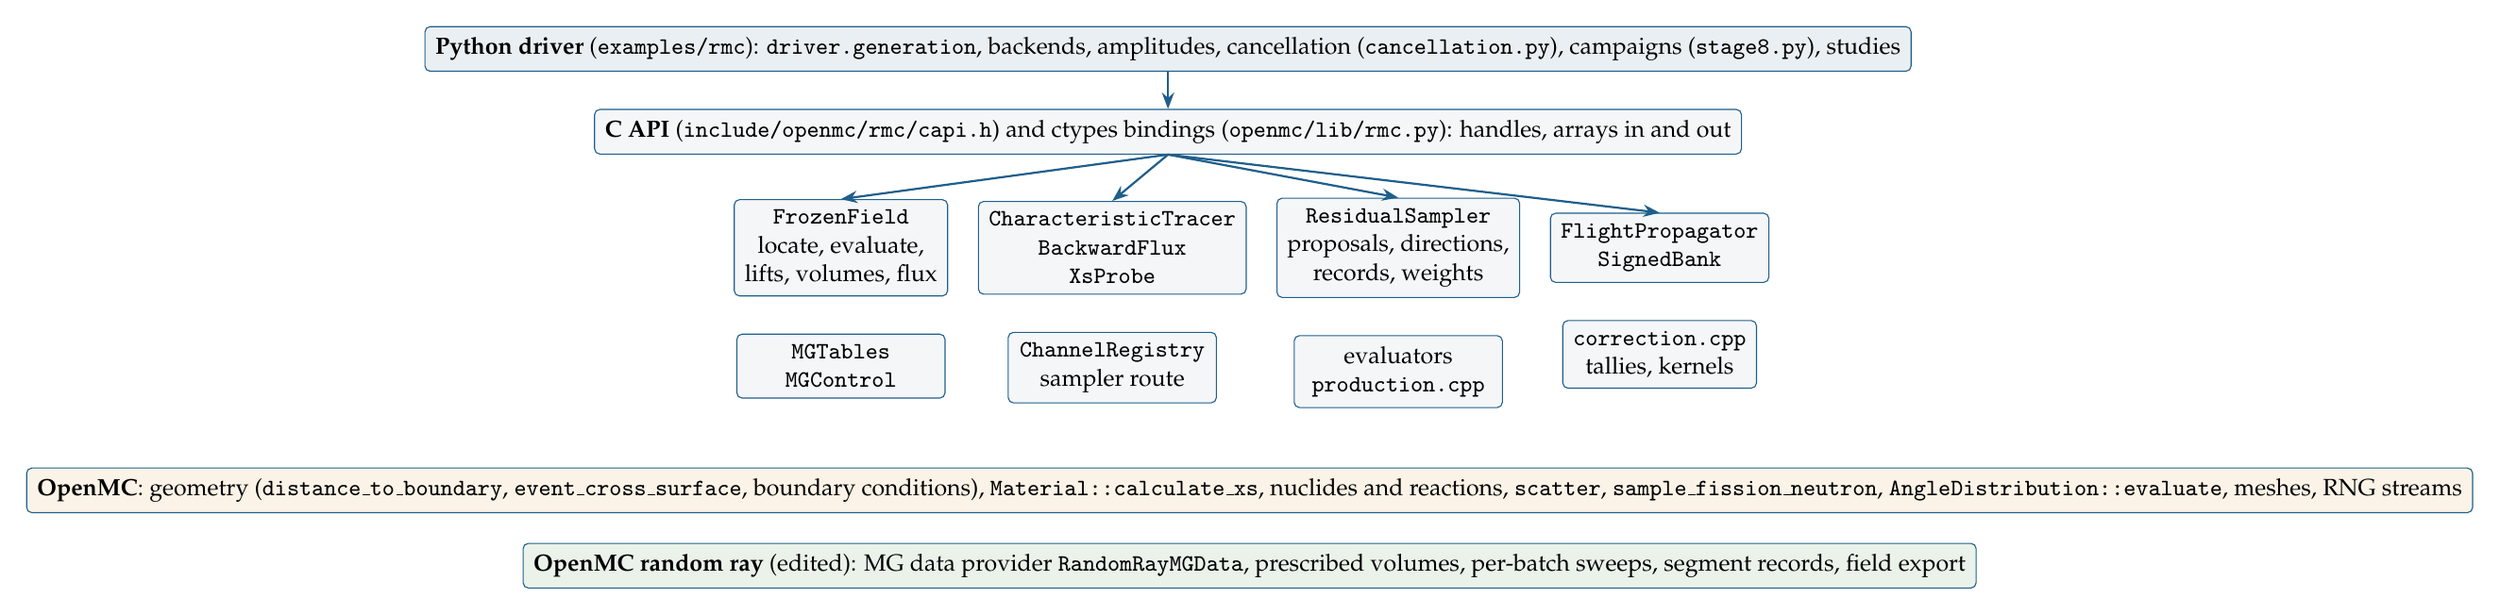
\begin{tikzpicture}[node distance=4mm and 6mm, every node/.style={font=\footnotesize}]
\node[box,minimum width=118mm,fill=headblue!10] (py) {\textbf{Python driver} (\code{examples/rmc}): \code{driver.generation}, backends, amplitudes,
cancellation (\code{cancellation.py}), campaigns (\code{stage8.py}), studies};
\node[box,below=5mm of py,minimum width=118mm] (capi) {\textbf{C API} (\code{include/openmc/rmc/capi.h}) and ctypes bindings (\code{openmc/lib/rmc.py}): handles, arrays in and out};
\node[box,below=6mm of capi,xshift=-44mm,minimum width=28mm] (field) {\code{FrozenField}\\ locate, evaluate,\\ lifts, volumes, flux};
\node[box,right=4mm of field,minimum width=28mm] (back) {\code{CharacteristicTracer}\\ \code{BackwardFlux}\\ \code{XsProbe}};
\node[box,right=4mm of back,minimum width=28mm] (res) {\code{ResidualSampler}\\ proposals, directions,\\ records, weights};
\node[box,right=4mm of res,minimum width=26mm] (fl) {\code{FlightPropagator}\\ \code{SignedBank}};
\node[box,below=5mm of back,minimum width=28mm] (chan) {\code{ChannelRegistry}\\ sampler route};
\node[box,below=5mm of res,minimum width=28mm] (prod) {evaluators\\ \code{production.cpp}};
\node[box,below=5mm of field,minimum width=28mm] (mg) {\code{MGTables}\\ \code{MGControl}};
\node[box,below=5mm of fl,minimum width=26mm] (corr) {\code{correction.cpp}\\ tallies, kernels};
\node[box,below=8mm of prod,xshift=-20mm,minimum width=118mm,fill=accorange!10] (omc) {\textbf{OpenMC}: geometry (\code{distance\_to\_boundary}, \code{event\_cross\_surface}, boundary conditions),
\code{Material::calculate\_xs}, nuclides and reactions, \code{scatter}, \code{sample\_fission\_neutron},
\code{AngleDistribution::evaluate}, meshes, RNG streams};
\node[box,below=4mm of omc,minimum width=118mm,fill=accgreen!10] (rr) {\textbf{OpenMC random ray} (edited): MG data provider \code{RandomRayMGData}, prescribed volumes,
per-batch sweeps, segment records, field export};
\draw[arr] (py)--(capi);
\foreach \n in {field,back,res,fl} \draw[arr] (capi.south) -- (\n.north);
\end{tikzpicture}
\caption{Module map. Python owns the outer loop; C++ owns every kernel that touches particles, and
reaches OpenMC's physics and geometry directly. The random-ray solver runs inside the same CE
process through a multigroup data provider.}\label{fig:impl:modules}
\end{figure}

Figure~\ref{fig:impl:modules} shows the structure. The decisions behind it:

\begin{enumerate}
\item \textbf{One CE process, with OpenMC's random ray as the MG sweep.} OpenMC loads either CE or MG
  data, never both. Random ray needs MG data only through a few small tables, so they were routed
  through a provider (\code{RandomRayMGData}) that is filled from the MG library in ordinary random ray
  and from the field file's exported tables in RMC. The random-ray paths do not compute CE cross
  sections, so they run unchanged in a CE process. Reuse buys ray sampling, segment attenuation, mesh
  subdivision, region lookup and threading; the regression tests guard the refactor (bitwise).
\item \textbf{OpenMC never sees a signed weight.} Every OpenMC routine receives a positive scratch
  particle of unit weight; signs, tags and yields live in \code{SignedBank} and the records. OpenMC's
  weight cutoff, roulette and \code{create\_fission\_sites} would all misbehave with negative weights.
\item \textbf{Python owns the loop, C++ the kernels.} Every kernel has a C entry point that pytest
  can call with chosen inputs; that is the seam for the gates. The cost is a copy of the bank across
  the boundary each generation, measured below.
\item \textbf{Records with deferred weights.} Residual generation returns scalar-free records; a
  separate step forms weights from $(a,b,k,c,\lambda)$. Pre-generated and run-time residuals are the
  same code; estimator variants are compared on identical samples.
\item \textbf{One random stream per sample and purpose.} Every sample and flight derives its seed from
  (base, generation, purpose, index) with OpenMC's skip-ahead LCG, so results do not depend on order
  or thread count, and replicas are just different base seeds.
\item \textbf{Every channel on exactly one route.} The registry partitions production by energy, so
  adding an evaluator for a reaction moves it across without touching the estimator.
\end{enumerate}

\section{Components, data containers and algorithms}\label{sec:impl:components}

\subsection{The field}

\code{FrozenField} reads the field file (regions keyed by cell, instance and mesh bin; group values;
group edges; MG tables), the lift file (fine grid and per-material histograms) and the volume file.
Lookups are flat arrays indexed \code{[(t*R + r)*G + g]}. \code{locate()} mirrors random ray's region
key (lowest cell, instance, mesh bin of the global position), so the CE process finds the same
regions. \code{evaluate()} is a bin search on the fine grid and two loads. Everything is
\code{const} after construction, so threads can share it.

\subsection{Tracing and the backward flux}

\code{CharacteristicTracer} owns a scratch \code{Particle} and moves it with
\code{distance\_to\_boundary()} and \code{event\_cross\_surface()} (which applies reflective and
periodic conditions), splitting each cell crossing at source-region mesh crossings exactly as
\code{RandomRay::attenuate\_flux()} does. It is resumable: \code{begin(r,u)} then \code{extend(n)}
returns segments in chunks. \code{SegmentList} is a structure of arrays reused across calls (no
allocation in steady state). \code{BackwardFlux::evaluate\_all} walks one path for a list of energies,
with per-energy roulette, and optionally MG accumulators for the control on the same segments.

\begin{algorithm}[h]
\caption{Backward $\psi$ for several energies on one path}\label{alg:psi}
\DontPrintSemicolon
\KwIn{$\vr^\star$, $\vO'$, energies $E'_1..E'_n$, tail options}
tracer.begin($\vr^\star$, $-\vO'$); $T_e\gets1$, $\psi_e\gets0$, alive$_e\gets$ true for all $e$\;
\While{some energy alive}{
  segs $\gets$ tracer.extend(32)\;
  \ForEach{segment $k$ in segs}{
    \ForEach{alive energy $e$}{
      $\Sigma\gets$ \code{XsProbe.total}(mat$_k$, $E'_e$)\tcp*{the hot spot}
      $\psi_e \mathrel{+}= T_e\,Q^F(R_k,E'_e)\,(1-e^{-\Sigma\ell_k})/\Sigma$;\quad $T_e\mathrel{*}=e^{-\Sigma\ell_k}$\;
      \lIf{$T_e<T_c$}{survive with prob.\ $T_e/T_c$ and set $T_e\gets T_c$, else alive$_e\gets$ false}
    }
  }
  \lIf{path ended in vacuum}{stop}
}
\end{algorithm}

\code{XsProbe} wraps \code{Material::calculate\_xs} on a scratch particle: the lookup runs OpenMC's
own code (energy grid search on the logarithmic hash grid, interpolation, per-nuclide loop), and
leaves every microscopic cross section in the particle's cache for the evaluators. It caches the
last (material, energy) pair, which helps when consecutive segments share both.

\subsection{Residual sampling}

\code{ResidualSampler::sample(tag, N, seed, records)} runs the loop of Section~\ref{sec:residual}.
Its proposals return \code{Draw<T>\{value, density\}}, so a weight can only be formed from the density
that was actually sampled. Directions come from a \code{DirectionSource} (isotropic Fibonacci under a
random rotation, or sweep segments by region). Records are a structure of arrays (\code{r, u, E,
density, tag, kind, channel, C\_s, C\_f, M\_s, M\_f, R\_s, R\_f, U, Z, E\_in, nuclide}), about 150
bytes per record.

\begin{algorithm}[h]
\caption{One residual sample (density route; tag $t$)}\label{alg:sample}
\DontPrintSemicolon
draw destination $\vr^\star$, locate region and material; draw $(E,\vO)$ with density $\varrho$\;
$U\gets\Qmg_t(\vr^\star,E)$\;
\ForEach{direction $j$ with weight $\omega_j$}{
  energies $\gets$ elastic images $E/\gamma_{A_i}(\mu_0)$ of each nuclide (tag $s$), a drawn $E'$ (tag $f$),
  $K$ drawn energies for the sampler route\;
  $\psi_s,\psi_f \gets$ \code{evaluate\_all}(path, energies) \tcp*{one trace}
  $C_y\mathrel{+}=\omega_j\,[\text{evaluator production at }(E,\vO)]\,\psi_y$\;
  \ForEach{sampler energy $E'_k$}{call OpenMC's routine; emit a particle at its outgoing state}
  $M_y\mathrel{+}=\omega_j\,q^{MG}_j$ (control)\;
}
$R_y\gets$ restored control mean ($L$ MG-only directions or sweep)\;
emit the density record $(\vr^\star,E,\vO,\varrho,C,M,R,U)$\;
\end{algorithm}

\subsection{Flights}

\code{FlightPropagator::propagate(bank, N, k, seed, out, tally, aux)} selects parents from a
cumulative $|w|$ array (binary search), flies a geometry particle to the sampled optical depth, and
collides with OpenMC's routines (Section~\ref{sec:flights}). The optional \code{FlightAux} records each
child's parent, path length and nuclide (for regional cancellation) and accumulates the collision
estimator of the fission rate by field region (for the correction tally).

\subsection{Cancellation and tallies}

Cancellation lives in Python (\code{cancellation.py}) with C++ kernels for the expensive parts:
\code{near\_kernel} (image enumeration and optical depth along each reflected straight path) and
\code{fission\_chi} (the fission emission density of a nuclide at an incident energy, partial
reactions weighted by cross section). Binned netting is a \code{bincount} over bin keys and a
vectorized re-sampler (rejection in the region's voxel). The correction tally's field part is
\code{field\_reaction\_tally} in C++; the bank part comes from the flights.

\begin{algorithm}[h]
\caption{Binned netting with an exact low term}\label{alg:netting}
\DontPrintSemicolon
key$_i\gets$ (tag, zone(region($\vr_i$)), group($E_i$), dirbin($\vO_i$))\;
$m_b\gets\sum_{\text{key}_i=b}w_i$ \;
\lIf{exact low}{$m_b\mathrel{-}=b_t\sum_{R\in Z}V_RQ_{t,R,g}/D$}
$e_b\gets N|m_b|/\sum|m|$;\quad $n_b\gets\lfloor e_b+\xi_b\rfloor$\tcp*{stochastic rounding}
\ForEach{bin $b$ with $n_b>0$}{draw $n_b$ states: region $\propto V_RQ_{t,R,g}$, uniform in it, lift in $E$, uniform in the direction bin; weight $m_b/e_b$}
\end{algorithm}

\subsection{Data containers}

\begin{table}[h]\centering\small
\begin{tabularx}{\textwidth}{>{\raggedright}p{3.2cm}>{\raggedright}p{4.6cm}X}
\toprule
Container & Layout & Why\\
\midrule
\code{FrozenField} & flat \code{vector<double>} \code{[2][R][G]}, lifts \code{[2][M][F]}, hash map key$\to$region & cache-friendly, \code{const}, shared by threads\\
\code{SegmentList} & structure of arrays (length, material, $\sqrt{kT}$, density multiplier, region) & reused per thread, no allocation in steady state\\
\code{ResidualRecords} & structure of arrays, one entry per record; 16 columns & deferred weights: amplitudes enter only at weighting\\
\code{SignedBank} & structure of arrays (\code{x,y,z,ux,uy,uz,E,w,tag}) & selection by $|w|$ and tag sums touch one or two arrays\\
\code{FlightAux} & per child (parent, path, nuclide); per region tallies & exact cancellation and the correction tally\\
Python banks & dicts of \code{numpy} arrays & vectorized netting and resampling; copied into C++ for flights\\
\bottomrule
\end{tabularx}
\caption{Data containers.}\label{tab:impl:containers}
\end{table}

\subsection{Determinism, threads and tests}

Every sample and flight derives its random stream from its index with OpenMC's skip-ahead
(\code{future\_seed}), so a kernel's output is a function of its inputs and seed alone, regardless of
order. The kernels are not threaded yet; with thread-local scratch (\code{XsProbe}, \code{SegmentList},
\code{Particle}) and outputs merged in index order they become bitwise reproducible for any thread count.
The test suite (\code{tests/rmc}, 170 tests, about 15 minutes on two cores) runs every gate of
Appendix~\ref{app:gates} through the C API with chosen inputs; each statistical gate has a deliberate
mutation that makes it fail.

\section{Performance}\label{sec:impl:performance}

\subsection{Where the time goes now}

Table~\ref{tab:impl:time} (from the Stage 8 runs, Section~\ref{sec:res:stage8}) splits a generation
into its kernels. Residual sampling dominates; within it, the cross-section lookups on backward
segments (\code{calculate\_xs} per segment and energy) are the hot spot, as the cost model predicts.

\subsection{What each design choice costs, and what optimization can recover}\label{sec:impl:projection}

\begin{itemize}
\item \textbf{Cross sections per segment and energy.} Each lookup is a full
  \code{Material::calculate\_xs}: a grid search per nuclide, interpolation of every reaction, and
  S($\alpha,\beta$) and probability-table logic. The backward flux needs only $\Sigma_t$ (and a few
  production cross sections at the collision energies). A total-only lookup on a material-union grid
  with a per-path (material, energy) cache would cut this by an estimated 3--6 times; images of the
  same nuclide set repeat energies across directions.
\item \textbf{One trace per direction, many energies.} Already exploited; the elastic images add one
  energy per nuclide per direction. Sampling one nuclide per direction (channel sampling) would cut
  $n_E$ from the number of nuclides to one, at a small variance cost.
\item \textbf{Python orchestration.} Bank copies across the C API, per-particle Python loops in
  pooling and regional cancellation, and \code{numpy} netting cost 5--15\% of a generation at these
  sizes and grow linearly; moving them to C++ removes most of it.
\item \textbf{Threads.} Every kernel is embarrassingly parallel over samples and flights with
  per-sample seeds. The measurements here are single-threaded, as is the reference, so the comparison
  is fair; threading scales both.
\item \textbf{Algorithmic, not engineering.} The residual's per-sample variance (Section
  \ref{sec:res:controlled}) and the bank's stationary $\Wabs$ set the floor; better evaluators (free gas,
  inelastic levels), better controls (P$_N$), and cancellation tuned to the representation move it.
\end{itemize}

\appendix
\section{Notation}\label{app:notation}

\begin{longtable}{>{\raggedright}p{3.2cm}p{11cm}}
\toprule
Symbol & Meaning\\
\midrule
$\vr,E,\vO$ & position, energy, direction; $x=(\vr,E,\vO)$ a point of phase space\\
$\psi,\phi$ & angular and scalar flux\\
$\Sigma_x,\sigma_x$ & macroscopic and microscopic cross section of reaction $x$\\
$Q_s,Q_f$ & emission density by scattering-type and fission reactions (tags $s$, $f$)\\
$\G,\mathcal P,\B$ & flight operator, collision operator, one generation $\B=\mathcal P\G$\\
$\K_t$ & CE production of tag $t$ from an emission density: $\mathcal P_t\G$\\
$k$, $k^{\mathrm{MG}}$ & eigenvalue estimate; the random-ray eigenvalue\\
$R$, $g$, $m$ & source region, energy group, material\\
$Q_{t,R,g}$ & MG emission per unit volume, integrated over angle and group\\
$h_{t,m,g}(E)$, $h^\phi$ & lifts: within-group emission and flux shapes\\
$\Qmg_t$ & the lifted field, eq.~\eqref{eq:field}; $Q^F=a_s\Qmg_s+a_f\Qmg_f$\\
$a,b$ & amplitudes of the field acting as source and of the field candidate kept\\
$\delta Q$ & the bank: signed CE particles\\
$\Wabs$ & absolute weight of a bank, $\sum_i|w_i|$\\
$\vr^\star,\varrho$ & residual destination; density of a record's state\\
$J,\omega_j$ & incident directions per destination and their weights\\
$K$, $g(E')$ & incident energies per direction on the sampler route; incident proposal\\
$C_y,M_y,R_y,U,Z$ & record terms: CE production from source tag $y$, MG control, its mean, field value, sampler control\\
$c,\lambda,L$ & control coefficient, mixing with the sweep emission, MG-only directions\\
$M_{II}$ & forward samples of the flux-difference region term\\
$N,N_\delta,N_B$ & residual samples per tag, flights, bank size after resampling\\
$f_n$ & fission production of generation $n$; $k_{n+1}=k_nf_n$\\
$K(\mathbf x\mid\mathbf x_p,E)$ & near point kernel of an isotropic parent\\
$\chi_m(E\mid E')$ & fission emission density of nuclide $m$\\
\bottomrule
\end{longtable}

\section{Gates and tests}\label{app:gates}

\begin{longtable}{>{\raggedright}p{1.4cm}>{\raggedright}p{6.2cm}p{6.6cm}}
\toprule
Gate & Quantity & Reference\\
\midrule
G0.1 & stationary-target kinematics & closed forms; mutation (Jacobian)\\
G1.0--G1.6 & field export, emission, lifts, locator, volumes, C++ field, field source & random-ray tallies; independent numpy recomputation; Python reference\\
G2.1--G2.6 & tracer, backward $\psi$, roulette, random ray in CE, segment records & analytic unfolded paths; infinite-medium closed form; MG process\\
G3.1--G3.3, G3.6 & channel partition; fission and elastic densities; MG control & total production; OpenMC samplers histogrammed; random-ray emission\\
G4.1--G4.4, G4.7 & residual mean (every estimator), proposal densities, linearity, deferred weights & OpenMC first-collision tallies with \code{CollisionFilter([1])}\\
G5.1--G5.4 & flights & homogeneous expectations; OpenMC with the bank as source\\
G6.1--G6.2 & iteration & deterministic toy to $10^{-12}$; one generation against OpenMC\\
G8.0 & near kernel & histogram of fission children of a point parent\\
G8.1 & regional cancellation is exact & binned means with and without, independent flights\\
G8.2 & destination pooling is exact & binned means with and without\\
G8.3 & binned netting & bin totals plus the closed-form low term\\
G8.4 & field part of the correction tally & collision estimator of forward flights of the field\\
\bottomrule
\end{longtable}

\section{Glossary}

\begin{description}[style=nextline,leftmargin=2.2cm,font=\normalfont\bfseries]
\item[bank] signed CE particles carrying the correction $\delta Q$
\item[channel] one reaction of one nuclide with outgoing neutrons, with its tag and route
\item[destination] the point where a residual sample is evaluated
\item[evaluator] a density of a production kernel at a chosen outgoing state
\item[field] the multigroup emission lifted to continuous energy
\item[flight] one forward CE flight of a bank particle to its next collision
\item[image] the incident energy that elastic (or two-body) kinematics map to a given output
\item[lift] a within-group energy shape tallied from CE
\item[netting] summing signed weights per bin and re-sampling the net
\item[pooling] moving a known part of a particle's density into a shared distribution where signs cancel exactly
\item[record] a residual sample stored without amplitudes, weighted later
\item[residual] $\B Q^F-F$: the field's one-generation CE emission minus what is kept
\item[roulette] unbiased termination of a backward path's tail
\item[route] evaluator (density) or sampler (OpenMC's routine) for a channel
\item[tag] $s$ (scattering-born) or $f$ (fission-born) emission
\end{description}

\end{document}
